% Livro de apoio - Engenharia da Qualidade e Confiabilidade
% Baseado nos slides da aula de Introdução
\documentclass[12pt,a4paper]{report}

\usepackage[utf8]{inputenc}
\usepackage[T1]{fontenc}
\usepackage[portuguese]{babel}
\usepackage{amsmath, amssymb, amsfonts}
\usepackage{lmodern}
\usepackage{graphicx}
\usepackage{tikz}
\usepackage{pgfplots}
\pgfplotsset{compat=1.18}
\usetikzlibrary{arrows.meta,positioning,shapes.multipart,shapes.geometric,calc,fit}
\usetikzlibrary{shapes.gates.logic.US, positioning}

\usepackage{hyperref}
\usetikzlibrary{decorations.pathreplacing} % necessário para os braces
\usepackage[most]{tcolorbox}
\newtcolorbox{block}[1]{%
  colback=green!5,
  colframe=maincolor,
  coltitle=white,
  title=#1,
  fonttitle=\bfseries,
  boxrule=1.5pt,
  arc=3mm,
  left=6pt,
  right=6pt,
  top=6pt,
  bottom=6pt
}
\usepackage[backend=biber, style=abnt, sorting=nyt, language=portuguese, url=true]{biblatex}
\addbibresource{referencias.bib}
\usepackage{setspace} 
\usepackage{geometry}
\usepackage{booktabs}
\usepackage{enumitem}
\usetikzlibrary{calc}
\geometry{
  a4paper,
  left=3cm,
  right=2cm,
  top=3cm,
  bottom=2.5cm
}

\onehalfspacing
\usepackage{listings}
\usepackage{xcolor}

% Configuração para o Python ficar com "cara" de código
\lstset{
    inputencoding=utf8,
    extendedchars=true,
    basicstyle=\ttfamily\small,
    keywordstyle=\color{blue}\bfseries,
    stringstyle=\color{green!50!black},
    commentstyle=\color{gray},
    numbers=left,
    numberstyle=\tiny\color{gray},
    stepnumber=1,
    frame=single,
    breaklines=true,
    postbreak=\mbox{\textcolor{red}{$\hookrightarrow$}\space},
    showstringspaces=false,
    literate={á}{{\'a}}1 {ã}{{\~a}}1 {ç}{{\c{c}}}1 {õ}{{\~o}}1 % Suporte a PT-BR no código
}
\hypersetup{
  colorlinks=true, 
  linkcolor=blue,
  urlcolor=blue,
  citecolor=blue,
  pdftitle={Engenharia da Qualidade e Confiabilidade},
  pdfauthor={Prof. Me. Sergio Souza Novak}
}
% Cores institucionais
\definecolor{maincolor}{RGB}{0,100,50}
\definecolor{forestgreen}{RGB}{0,100,50}

% Cor institucional UniRV
\definecolor{verdeuni}{RGB}{0,102,51}
\definecolor{meuverde}{RGB}{0,128,0}
\definecolor{meuvermelhoescuro}{RGB}{139,0,0}
% Suporte a texto justificado dentro de ambientes especiais
\usepackage{ragged2e}

% =======================
% Ambiente de cartão de autor
% =======================
\newenvironment{authorcard}{%
  \begin{minipage}[t]{\linewidth}\vspace{0pt}%
}{%
  \end{minipage}%
}

% Foto do autor (com fallback se o arquivo não existir)
\newcommand{\authorphoto}[1]{%
  \IfFileExists{#1}{%
    \includegraphics[width=2.8cm, height=3.5cm, keepaspectratio]{#1}%
  }{%
    \fbox{\parbox[c][3.5cm][c]{2.8cm}{\centering\color{gray}\small Foto}}%
  }%
}

% =======================
% Capa Estilo Tanenbaum
% =======================
\newcommand{\makecapa}{%
  \begin{titlepage}
    \thispagestyle{empty}
    \begin{tikzpicture}[remember picture, overlay]
      % Faixa Superior
      \fill[verdeuni]
        (current page.north west)
        rectangle ++(\paperwidth,-6.5cm);
      % Texto do Topo: Autores e Título
      \node[anchor=north, text width=\paperwidth, align=center]
        at ([yshift=-1.5cm]current page.north) {%
          {\Large\sffamily\color{white} SERGIO SOUZA NOVAK,\ \ ADRIANO S. de O. BAILÃO}\\[0.8cm]
          {\Huge\bfseries\sffamily\color{yellow} Tópicos em Confiabilidade e Qualidade de Software}\\[0.4cm]
          {\Large\sffamily\color{white} 1\textordfeminine{} EDI\c{C}\~{A}O}%
        };
      % Imagem Central
      \node[anchor=center] at ([yshift=-2.2cm]current page.center) {%
        \IfFileExists{figura_da_capa.png}{%
          \includegraphics[width=1.02\paperwidth]{figura_da_capa.png}%
        }{%
          \begin{tikzpicture}
            \fill[verdeuni!20] (0,0) rectangle (16cm,10cm);
            \node[font=\Huge\bfseries\sffamily, color=verdeuni!60!black] at (8cm,5cm)
              {Engenharia da Qualidade};
          \end{tikzpicture}%
        }%
      };
      % Faixa Inferior
      \fill[verdeuni] (current page.south west) rectangle ++(\paperwidth,2cm);
      % Logo UniRV
      \node[anchor=north] at ([yshift=-13cm]current page.center) {%
        \IfFileExists{Universidade_de_Rio_Verde.jpg}{%
        %   \includegraphics[width=4cm]{Universidade_de_Rio_Verde.jpg}%
        }{%
        %   {\color{white}\bfseries\large UniRV — Universidade de Rio Verde}%
        }%
      };
    \end{tikzpicture}
  \end{titlepage}%
}

% =======================
% Página de Autores
% =======================
\newcommand{\authorpage}{%
\newpage
\thispagestyle{empty}
\begin{tikzpicture}[remember picture, overlay]
  \fill[verdeuni]
    (current page.north west)
    rectangle (current page.south east);
  \node at ([yshift=-1.8cm]current page.north) {%
    \IfFileExists{Universidade_de_Rio_Verde.jpg}{%
      \includegraphics[width=5cm]{Universidade_de_Rio_Verde.jpg}%
    }{%
      {\color{white}\bfseries\Large UniRV}%
    }%
  };
\end{tikzpicture}
\vspace*{4.5cm}
\begin{center}
{\color{white}\bfseries\LARGE Conhe\c{c}a os Autores}

\vspace{1.5cm}

\begin{tabular}{ccc}

% Autor 1
\begin{minipage}[t]{0.30\textwidth}
\begin{authorcard}
\centering
{\small\bfseries\color{white} Sergio Souza Novak}

\vspace{0.6cm}

\authorphoto{foto_sergio.jpeg}

\vspace{0.7cm}

\justifying\footnotesize\color{white}
Sergio Souza Novak é Mestre em Ciências Agrárias pelo Instituto Federal Goiano.
Atua nas áreas de Banco de Dados, Inteligência Artificial e Desenvolvimento de
Software, com experiência acadêmica e industrial e publicações científicas
aplicadas à agricultura digital.
\end{authorcard}
\end{minipage}

&

% Autor 2
\begin{minipage}[t]{0.30\textwidth}
\begin{authorcard}
\centering
{\small\bfseries\color{white} Ronaldo}

\vspace{0.6cm}

\authorphoto{foto_sergio.jpeg}

\vspace{0.7cm}

\justifying\footnotesize\color{white}
Lorem ipsum dolor sit amet, consectetur adipiscing elit. Donec a diam lectus.
Sed sit amet ipsum mauris. Maecenas congue ligula ac quam viverra nec
consectetur ante hendrerit.
\end{authorcard}
\end{minipage}

&

% Autor 3
\begin{minipage}[t]{0.30\textwidth}
\begin{authorcard}
\centering
{\small\bfseries\color{white} Leandro}

\vspace{0.6cm}

\authorphoto{foto_sergio.jpeg}

\vspace{0.7cm}

\justifying\footnotesize\color{white}
Leandro possui experiência em computação aplicada, análise de sistemas e
desenvolvimento tecnológico, participando de projetos acadêmicos e educacionais.
\end{authorcard}
\end{minipage}

\end{tabular}
\end{center}
\newpage%
}
\newtcolorbox{resposta}[1]{%
  colback=white,
  colframe=forestgreen!30,
  arc=1mm,
  height=#1,
  width=\textwidth,
  boxrule=0.8pt
}

\begin{document}


\makecapa
% \authorpage

\tableofcontents
\clearpage

\chapter{Introdução à Engenharia da Qualidade}

A Engenharia da Qualidade é uma área da engenharia dedicada ao planejamento,
ao controle, à garantia e à melhoria da qualidade de produtos, serviços e
processos. Enquanto a qualidade era, historicamente, tratada de forma
predominantemente \emph{inspetiva} --- isto é, por meio de inspeções ao final
do processo produtivo --- a Engenharia da Qualidade traz uma abordagem
proativa, baseada em métodos científicos, estatística e pensamento sistêmico.

\begin{figure}[h]
    \centering
    \begin{tikzpicture}[node distance=2cm, auto]
        \node[draw, rectangle, fill=red!10, text width=4cm, align=center] (insp) {Abordagem Inspetiva \\ (Histórica)};
        \node[draw, rectangle, fill=green!10, text width=4cm, align=center, right=of insp] (eng) {Engenharia da Qualidade \\ (Proativa)};
        
        \node[below=0.5cm of insp, font=\small, text width=4cm, align=center] {Foco no final; \\ Corretiva; \\ Reativa a falhas.};
        \node[below=0.5cm of eng, font=\small, text width=4cm, align=center] {Foco no projeto; \\ Preventiva; \\ Melhoria contínua.};
        
        \draw[->, ultra thick] (insp) -- (eng) node[midway, above] {Evolução};
    \end{tikzpicture}
    \caption{Evolução da gestão da qualidade: do modelo reativo ao proativo.}
\end{figure}

O ponto de partida é a compreensão de que \textbf{qualidade não é um acaso},
mas sim o resultado de processos bem projetados e bem controlados. Um produto
ou serviço de qualidade é aquele que atende aos requisitos explícitos
especificados em normas, contratos e regulamentos; que satisfaz às expectativas
implícitas dos clientes, muitas vezes não completamente formalizadas; que
apresenta desempenho consistente ao longo do tempo, com baixa variabilidade e
taxa reduzida de falhas; e que é produzido de forma eficiente, com mínimo
despídio de recursos.

\begin{figure}[h]
    \centering
    \begin{tikzpicture}[
        every node/.style={draw, circle, fill=blue!5, align=center, font=\small, inner sep=5pt},
        center node/.style={fill=blue!20, font=\bfseries, inner sep=10pt}
    ]
        \node[center node] (c) {Qualidade do\\Produto};
        \node[above=of c] (r) {Requisitos\\Explicitos};
        \node[below=of c] (e) {Eficiência de\\Produção};
        \node[left=of c] (x) {Expectativas\\do Cliente};
        \node[right=of c] (v) {Baixa\\Variabilidade};
        
        \draw[thick] (c) -- (r);
        \draw[thick] (c) -- (e);
        \draw[thick] (c) -- (x);
        \draw[thick] (c) -- (v);
    \end{tikzpicture}
    \caption{Os quatro pilares de um produto ou serviço de qualidade.}
\end{figure}

Do ponto de vista da organização, a Engenharia da Qualidade também está
fortemente ligada à competitividade. Empresas que dominam as ferramentas e
conceitos de qualidade tendem a lançar produtos mais confiáveis e atraentes,
reduzindo custos de retrabalho, garantia e suporte. Com isso, ganham reputação
positiva junto aos clientes e se diferenciam em mercados cada vez mais
exigentes.

\section{Qualidade e Confiabilidade}

\subsection{Definições Básicas}

Embora intimamente relacionadas, qualidade e confiabilidade não são sinônimos.
De forma simplificada, podemos dizer que \textbf{qualidade} está associada ao
grau em que um produto ou serviço atende às especificações e às expectativas
do cliente \emph{no momento em que é entregue}. Já a \textbf{confiabilidade}
diz respeito à capacidade desse produto ou serviço de manter seu desempenho
adequado \emph{ao longo do tempo}, sob condições de uso específicas. Enquanto
a qualidade pode ser observada num instante, a confiabilidade é necessariamente
uma propriedade temporal.

\begin{figure}[h]
    \centering
    \begin{tikzpicture}[thick]
        \draw[->] (0,0) -- (8,0) node[right] {Tempo};
        \draw[fill=blue!20] (0,0.5) rectangle (1,2) node[midway] {Qualidade};
        \draw[fill=green!20] (1,0.5) rectangle (7,2) node[midway] {Confiabilidade};
        
        \node[below] at (0.5, 0.5) {Entrega};
        \node[below] at (4, 0.5) {Uso contínuo em produção};
        
        \node[align=center, font=\small] at (0.5, 2.5) {Atendimento a\\especificações};
        \node[align=center, font=\small] at (4, 2.5) {Manutenção do desempenho sob condições normais};
    \end{tikzpicture}
    \caption{Qualidade (foco no momento da entrega) versus Confiabilidade (foco na duração).}
\end{figure}

Por exemplo, um sistema de software pode ser entregue com todas as
funcionalidades combinadas (alta qualidade inicial), mas, se apresentar
falhas frequentes em produção, terá baixa confiabilidade. Em contrapartida,
um sistema levemente limitado em funcionalidades mas extremamente estável
pode ser percebido como mais confiável e, em muitos contextos, mais valioso.

Ao longo desta disciplina, exploraremos justamente essa interseção entre
qualidade de software, confiabilidade operacional e práticas modernas de
engenharia, como o \emph{Site Reliability Engineering} (SRE) adotado pelo
Google \cite{beyer2016sre, googlesre2024}.

\subsection{Qualidade ao Longo do Tempo}

\section{Áreas de Atuação da Engenharia da Qualidade}

\subsection{Setores em que a Qualidade é Crítica}

A Engenharia da Qualidade está presente em uma ampla variedade de setores
econômicos. Tradicionalmente, associamos qualidade à indústria de
manufatura, mas hoje ela é igualmente crítica nos \textbf{serviços} (bancos,
hospitais, telecomunicações, educação, transporte), no \textbf{agronegócio}
(controle de qualidade em insumos, produção, armazenagem e logística), na
\textbf{Tecnologia da Informação} (desenvolvimento e operação de sistemas,
aplicativos, plataformas em nuvem e serviços digitais) e no \textbf{setor
público} (políticas de qualidade em serviços governamentais, transparência e
foco no cidadão).

Em todos esses contextos, a Engenharia da Qualidade oferece ferramentas para
mapear processos e identificar pontos críticos, medir desempenho por meio de
indicadores, reduzir variabilidade e desperdícios, promover a melhoria contínua
(\emph{kaizen}) e apoiar a tomada de decisão baseada em dados.

No contexto específico da Engenharia de Software, a qualidade se manifesta,
por exemplo, na definição de requisitos claros, na aplicação de boas práticas
de desenvolvimento, na realização de testes sistemáticos e na operação
confiável em produção.


\section{O Programa Apollo e a Engenharia de Confiabilidade}

\subsection{Contexto Histórico}

Um dos exemplos históricos mais interessantes na área de confiabilidade é o
trabalho de \textbf{Margaret Hamilton} no programa Apollo, da NASA \cite{hamilton1976apollo, fisher2019moon}. Ela foi
uma das engenheiras de software responsáveis pelo desenvolvimento dos sistemas
de bordo utilizados nas missões que levaram o ser humano à Lua \cite{garman2011apollo}.

\subsection{Margaret Hamilton e o Pensamento de Confiabilidade}

Margaret Hamilton liderou a equipe de desenvolvimento de software no
Laboratório de Instrumentação do MIT. Em uma época em que o termo
``engenharia de software'' ainda estava sendo definido, ela já defendia
práticas rigorosas de projeto, verificação e tratamento de falhas --- conceitos
que hoje associamos diretamente à Engenharia de Confiabilidade e à SRE.

Seu trabalho enfatizava:
\begin{itemize}[nosep]
    \item a necessidade de \textbf{antecipar erros humanos} e falhas de
    operação;
    \item a importância de projetar sistemas que tolerem condições inesperadas;
    \item a criação de mecanismos de recuperação capazes de evitar que
    pequenos erros levem a desastres catastróficos.
\end{itemize}

\subsection{O Episódio no Simulador de Missão}

Um episódio marcante ocorreu durante testes no simulador do Apollo. Margaret
levou sua filha Lauren ao trabalho, e, em determinado momento, a criança
pressionou teclas do painel de controle (DSKY) de forma aleatória. Essa
interação aparentemente inocente resultou na falha de uma missão simulada.

Do ponto de vista de engenharia, o episódio foi revelador:
\begin{itemize}[nosep]
    \item mostrou que era possível ativar, de maneira inadvertida, programas
    de navegação em momentos inadequados;
    \item evidenciou que erros simples de operação podiam ter consequências
    graves;
    \item indicou a necessidade de mecanismos adicionais de proteção.
\end{itemize}

Em vez de culpar o ``usuário'' (no caso, a criança), Hamilton interpretou o
ocorrido como um \textbf{sintoma de fragilidade do sistema}. Essa postura é
central em abordagens modernas de confiabilidade: em vez de supor que os
operadores nunca erram, assume-se que erros humanos são inevitáveis e que o
sistema deve ser projetado para lidar com isso.

\begin{figure}[h]
    \centering
    \begin{tikzpicture}[
        block/.style={draw, rounded corners, fill=blue!8, minimum width=3cm, minimum height=1cm, align=center, font=\small},
        alert/.style={draw, rounded corners, fill=red!15, minimum width=3cm, minimum height=1cm, align=center, font=\small},
        arrow/.style={->, thick, >=stealth}
    ]
    % Nós
    \node[block] (lauren) {Lauren pressiona\\teclas do DSKY};
    \node[block, right=1.8cm of lauren] (p01) {Programa \textbf{P01}\\é ativado};
    \node[alert, right=1.8cm of p01] (nav) {Dados de navegação\\são apagados};
    \node[alert, below=1.2cm of nav] (falha) {Missão simulada\\\textbf{FALHA}};
    \node[block, fill=green!12, below=1.2cm of lauren] (hamilton) {Hamilton:\\``O sistema é frágil,\\não o usuário.''};
    % Setas
    \draw[arrow] (lauren) -- (p01);
    \draw[arrow] (p01) -- (nav);
    \draw[arrow] (nav) -- (falha);
    \draw[arrow, dashed, green!50!black] (falha) -| (hamilton);
    \end{tikzpicture}
    \caption{Fluxo do episódio no simulador: uma ação inocente desencadeou uma falha catastrófica, revelando fragilidades no design.}
\end{figure}

\subsection{O Problema Técnico Identificado}

A falha estava relacionada à seleção acidental do programa \textbf{P01}, que
limpava os dados de navegação. Sem esses dados, o computador de bordo não
conseguia pilotar a nave, o que, em uma missão real, poderia impedir o retorno
à Terra.

Portanto, um simples comando, executado em um momento indevido, tinha
potencial para comprometer toda a missão. Em termos de Engenharia de
Confiabilidade, trata-se de um \emph{ponto único de falha} (\emph{single point
of failure}) altamente sensível a erro humano.

\begin{figure}[h]
    \centering
    \begin{tikzpicture}[
        comp/.style={draw, rounded corners, fill=cyan!10, minimum width=1cm, minimum height=1cm, align=center, font=\small},
        spof/.style={draw, very thick, rounded corners, fill=red!25, minimum width=3cm, minimum height=1.2cm, align=center, font=\small\bfseries},
        arrow/.style={->, thick, >=stealth}
    ]
    \node[comp] (astro) {Astronauta};
    \node[comp, right=0.5cm of astro] (dsky) {Painel DSKY};
    \node[spof, right=0.5cm of dsky] (p01) {Programa P01\\(Limpa Navegação)};
    \node[comp, right=0.5cm of p01] (agc) {Computador AGC};
    \node[comp, right=0.5cm of agc] (nav) {Navegação\\e Retorno};
    % Setas
    \draw[arrow] (astro) -- (dsky);
    \draw[arrow] (dsky) -- (p01);
    \draw[arrow] (p01) -- node[above, font=\tiny, red] {sem dados!} (agc);
    \draw[arrow, dashed, red] (agc) -- node[above, font=\tiny, red] {FALHA} (nav);
    % Ícone SPOF
    \node[below=0.3cm of p01, font=\footnotesize, red!70!black] {$\bigotimes$ Single Point of Failure};
    \end{tikzpicture}
    \caption{Ponto Único de Falha: a execução acidental do P01 era o elo mais fraco de toda a cadeia de navegação do Apollo.}
\end{figure}

\subsection{A Proposta de Solução de Margaret Hamilton}

Com mentalidade que hoje reconheceríamos como típica de SRE, Margaret
propôs a inclusão de:
\begin{itemize}[nosep]
    \item um código de verificação de erro que detectasse o uso indevido
    do programa P01;
    \item bloqueios que impedissem a execução desse programa em fases
    críticas do voo;
    \item mecanismos de recuperação automática caso o comando fosse, ainda
    assim, acionado.
\end{itemize}

Sua proposta, entretanto, foi inicialmente rejeitada sob o argumento de que
os astronautas eram altamente treinados e, portanto, não cometeriam esse tipo
de engano. Essa confiança excessiva nos operadores contrasta com a visão
contemporânea de SRE, que parte do princípio oposto: \textbf{erros humanos
sempre acontecerão}.


\begin{figure}[h]
    \centering
    \begin{tikzpicture}[
        layer/.style={draw, rounded corners, minimum width=10cm, minimum height=1.1cm, align=center, font=\small},
        arrow/.style={->, thick, >=Stealth}
    ]
    % Camadas de defesa
    \node[layer, fill=green!15] (l1) at (0,0) {\textbf{Camada 1:} Verificação de Erro --- Detectar uso indevido do P01};
    \node[layer, fill=yellow!15] (l2) at (0,-1.6) {\textbf{Camada 2:} Bloqueio --- Impedir P01 em fases críticas do voo};
    \node[layer, fill=orange!15] (l3) at (0,-3.2) {\textbf{Camada 3:} Recuperação Automática --- Restaurar dados se P01 for acionado};

    % Ação do astronauta
    \node[draw, circle, fill=blue!10, font=\small] (astro) at (0,4) {Astronauta executa P01};

    % Setas
    \draw[arrow] (astro) -- (l1);
    \draw[arrow, dashed] (l1) -- node[right, font=\tiny] {se passar} (l2);
    \draw[arrow, dashed] (l2) -- node[right, font=\tiny] {se passar} (l3);

    % Etiquetas
    \node[right=0.3cm of l1, font=\footnotesize, green!50!black] {$\checkmark$ Detecta};
    \node[right=0.3cm of l2, font=\footnotesize, yellow!60!black] {$\checkmark$ Bloqueia};
    \node[right=0.3cm of l3, font=\footnotesize, orange!70!black] {$\checkmark$ Recupera};

    \end{tikzpicture}
    \caption{Camadas de defesa propostas por Margaret Hamilton: detecção, bloqueio e recuperação automática --- o modelo de ``Defesa em Profundidade''.}
\end{figure}

\subsection{O Incidente Real na Apollo 8}

Pouco tempo depois, durante a missão Apollo 8, o astronauta Jim Lovell
acabou selecionando o programa P01 por engano, o que apagou os dados de
navegação em plena missão. A situação foi crítica e exigiu um esforço
significativo da equipe em solo para recuperar as informações e salvar a
missão.

Esse incidente confirmou, de forma dramática, as preocupações de Margaret
Hamilton. A documentação detalhada do sistema e o preparo da equipe
permitiram que a missão fosse recuperada, mas o evento deixou claro que a
abordagem de ``confiar apenas na perfeição humana'' é insustentável em
sistemas de alta criticidade.

\subsection{Lições para a Engenharia Moderna e SRE}

O caso do programa Apollo ilustra princípios centrais que permeiam tanto a
Engenharia de Confiabilidade quanto a SRE:
\begin{itemize}[nosep]
    \item \textbf{Erros humanos são inevitáveis}: sistemas devem ser projetados
    assumindo que pessoas vão se enganar, pressionar o botão errado ou esquecer
    um procedimento.
    \item \textbf{Sistemas críticos devem ser resilientes}: uma única ação
    incorreta não pode levar, sozinha, a um desastre.
    \item \textbf{Documentação e preparação são vitais}: conhecer bem o sistema
    e manter registros atualizados aumenta as chances de recuperação.
    \item \textbf{Confiabilidade é requisito de projeto}: não se trata de um
    ``extra'' a ser considerado depois, mas de uma preocupação central desde a
    concepção do sistema.
\end{itemize}

Essas lições continuam extremamente atuais em um mundo em que sistemas
computacionais controlam desde operações bancárias até infraestrutura
crítica, como energia e telecomunicações.

\begin{figure}[h]
    \centering
    \begin{tikzpicture}[
        central/.style={draw, circle, fill=blue!15, minimum size=2.5cm, align=center, font=\small\bfseries},
        lesson/.style={draw, rounded corners, fill=gray!8, minimum width=3.5cm, minimum height=0.9cm, align=center, font=\footnotesize}
    ]
    % Centro
    \node[central] (centro) {Lições do\\Programa\\Apollo};
    % Lições
    \node[lesson, fill=red!10] (l1) at (90:3.8cm) {Erros humanos\\são \textbf{inevitáveis}};
    \node[lesson, fill=orange!10] (l2) at (0:4.5cm) {Sistemas críticos\\devem ser \textbf{resilientes}};
    \node[lesson, fill=green!10] (l3) at (270:3.8cm) {Documentação e preparo\\são \textbf{vitais}};
    \node[lesson, fill=cyan!10] (l4) at (180:4.5cm) {Confiabilidade é\\\textbf{requisito de projeto}};
    % Conexões
    \draw[thick, red!50!black] (centro) -- (l1);
    \draw[thick, orange!50!black] (centro) -- (l2);
    \draw[thick, green!50!black] (centro) -- (l3);
    \draw[thick, cyan!50!black] (centro) -- (l4);
    \end{tikzpicture}
    \caption{Mapa das lições fundamentais do Programa Apollo para a Engenharia de Confiabilidade moderna.}
\end{figure}

\section{Modelo Tradicional: Sysadmin, Dev e Ops}

\subsection{Separação entre Dev e Ops}

Historicamente, muitas organizações estruturaram suas equipes de tecnologia
em dois grandes grupos: \textbf{Desenvolvimento (Dev)} e \textbf{Operações
(Ops)}. Nesse modelo, os administradores de sistemas (\emph{sysadmins}) eram
responsáveis por manter serviços em funcionamento, enquanto os desenvolvedores
criavam novas funcionalidades.

\subsection{A Abordagem com Administradores de Sistemas}

No modelo tradicional, os sysadmins:
\begin{itemize}[nosep]
    \item integram componentes de software;
    \item implantam serviços em produção;
    \item monitoram servidores e redes;
    \item respondem a incidentes e realizam manutenções.
\end{itemize}

À medida que o serviço cresce em número de usuários, complexidade e
infraestrutura, costuma-se aumentar também o número de administradores de
sistemas. Dessa forma, o custo operacional tende a crescer aproximadamente de
forma linear com a escala do serviço.

\begin{figure}[h]
    \centering
    \begin{tikzpicture}
        \begin{axis}[
            width=11cm, height=6cm,
            title={Custo Operacional no Modelo Sysadmin},
            xlabel={Escala do Serviço (usuários)},
            ylabel={Custo Operacional (equipe)},
            xmin=0, xmax=10, ymin=0, ymax=10,
            xtick={2,4,6,8,10},
            xticklabels={10k, 50k, 100k, 500k, 1M},
            ytick={2,4,6,8,10},
            yticklabels={2, 4, 6, 8, 10 sysadmins},
            grid=major,
            every axis title/.style={at={(0.5,1.05)}, font=\small\bfseries}
        ]
        % Linha linear
        \addplot[thick, red, mark=square*, mark size=2pt] coordinates {
            (1,1) (2,2) (4,4) (6,6) (8,8) (10,10)
        };
        \addlegendentry{Modelo Sysadmin (linear)}
        % Linha ideal sublinear
        \addplot[thick, green!60!black, mark=triangle*, mark size=2pt, dashed] coordinates {
            (1,1) (2,1.4) (4,2) (6,2.5) (8,2.8) (10,3)
        };
        \addlegendentry{Modelo ideal (sublinear)}
        \end{axis}
    \end{tikzpicture}
    \caption{No modelo tradicional, o crescimento do serviço exige crescimento proporcional da equipe de operações, enquanto modelos baseados em automação (como SRE) escalam de forma sublinear.}
\end{figure}

Entre as vantagens desse modelo, podemos destacar:
\begin{itemize}[nosep]
    \item paradigma amplamente conhecido;
    \item facilidade de contratação de profissionais;
    \item existência de ferramentas consolidadas de administração de sistemas;
    \item separação clara de responsabilidades entre quem ``constrói'' e quem
    ``opera''.
\end{itemize}

Por outro lado, o modelo gera conflitos importantes, especialmente em
organizações que precisam inovar com rapidez.

\subsection{Conflitos Estruturais entre Dev e Ops}

A equipe de desenvolvimento, de maneira geral, é avaliada pela velocidade com
que entrega novas funcionalidades e responde a demandas de negócio. Já a
equipe de operações é cobrada pela estabilidade, disponibilidade e ausência
de incidentes em produção.

Assim, emergem objetivos que podem ser conflitantes:
\begin{itemize}[nosep]
    \item \textbf{Dev} quer mudar o sistema com frequência para inovar;
    \item \textbf{Ops} prefere mudanças raras, cuidadosamente controladas, para preservar a estabilidade.
\end{itemize}

\begin{figure}[h]
    \centering
    \begin{tikzpicture}[thick, node distance=2.2cm]
        % Blocos Dev e Ops
        \node[draw, rounded corners, minimum width=3cm, minimum height=2cm, fill=blue!10, align=center] (dev) {\textbf{Desenvolvimento}\\\footnotesize Escreve código\\\footnotesize Cria features};
        \node[draw, rounded corners, minimum width=3cm, minimum height=2cm, fill=red!10, align=center, right=3.5cm of dev] (ops) {\textbf{Operações}\\\footnotesize Mantém servidores\\\footnotesize Responde incidentes};

        % Parede da Confusão
        \fill[gray!30] ($(dev.east)!0.5!(ops.west)$) ++(-0.4,-1.8) rectangle ++(0.8,3.6);
        \draw[dashed, very thick, gray!60] ($(dev.east)!0.5!(ops.west)$) ++(-0.4,-1.8) rectangle ++(0.8,3.6);
        \node[rotate=90, font=\bfseries\footnotesize, gray!70!black] at ($(dev.east)!0.5!(ops.west)$) {Parede da Confusão};

        % Metas acima
        \node[above=0.5cm of dev, font=\small\bfseries, blue!70!black] {Meta: \Large$\uparrow$ Velocidade};
        \node[above=0.5cm of ops, font=\small\bfseries, red!70!black] {Meta: \Large$\uparrow$ Estabilidade};

        % Setas de conflito
        \draw[->, ultra thick, blue!60!black] (dev.east) -- ($(dev.east)!0.48!(ops.west)$)
            node[midway, above, font=\scriptsize] {Deploys};
        \draw[->, ultra thick, red!60!black] (ops.west) -- ($(ops.west)!0.48!(dev.east)$)
            node[midway, above, font=\scriptsize] {Barreiras};

        % Resultado abaixo
        \node[below=2.5cm of $(dev.east)!0.5!(ops.west)$, draw, rounded corners, fill=yellow!15, align=center, font=\footnotesize] (resultado) {Resultado: Atrito, lentidão\\e culpabilização mútua};
        \draw[->, thick, gray] ($(dev.east)!0.5!(ops.west)$) ++(0,-1.8) -- (resultado);
    \end{tikzpicture}
    \caption{A ``Parede da Confusão'': Dev empurra código para produção enquanto Ops ergue barreiras para proteger a estabilidade, gerando atrito.}
    \label{fig:parede-confusao}
\end{figure}

Como a maioria das falhas e interrupções está associada a mudanças em
produção, a tendência natural de operações é criar barreiras, controles e
processos de aprovação mais rígidos. Isso pode levar a:
\begin{itemize}[nosep]
    \item comunicação indireta e pouco transparente;
    \item ciclos de lançamento mais longos e menos frequentes;
    \item sensação de ``guerra de trincheiras'', em que cada lado tenta
    defender seus interesses.
\end{itemize}

Na prática, o resultado é a redução da agilidade sem garantia de aumento
real de confiabilidade.

\subsection{Respostas Típicas ao Conflito}

Para contornar os processos de aprovação longos, as equipes de desenvolvimento
frequentemente:
\begin{itemize}[nosep]
    \item agrupam muitas mudanças em grandes \emph{releases}, o que aumenta o
    risco de cada implantação;
    \item utilizam \emph{feature flags} para ativar ou desativar recursos sem
    novo deploy;
    \item fragmentam o produto em múltiplos serviços menores, o que reduz o
    escopo de cada revisão, mas pode aumentar a complexidade geral do sistema.
\end{itemize}

Essas estratégias podem até aliviar alguns sintomas, mas não resolvem o
problema estrutural de fundo: a falta de alinhamento entre os objetivos de
desenvolvimento e de operações.

\begin{figure}[h]
    \centering
    \begin{tikzpicture}[
        block/.style={
            draw,
            rounded corners,
            fill=orange!10,
            minimum width=3.2cm,
            minimum height=0.9cm,
            text width=3.2cm,
            align=center,
            font=\footnotesize
        },
        arrow/.style={->, thick, >=Stealth}
    ]

    % Ciclo
    \node[block] (barr) at (90:2.8cm) {Ops cria mais\\barreiras e controles};
    \node[block] (acum) at (0:3.5cm) {Dev acumula\\mudanças em\\mega-releases};
    \node[block] (risco) at (270:2.8cm) {Deploys grandes\\= maior risco\\de falha};
    \node[block] (falha) at (180:3.5cm) {Falhas em\\produção\\aumentam};

    % Setas
    \draw[arrow, red!60!black] (barr) -- (acum);
    \draw[arrow, red!60!black] (acum) -- (risco);
    \draw[arrow, red!60!black] (risco) -- (falha);
    \draw[arrow, red!60!black] (falha) -- (barr);

    % Centro
    \node[font=\small\bfseries, red!70!black, align=center] at (0,0) {Ciclo\\Vicioso};

    \end{tikzpicture}
    \caption{O ciclo vicioso do modelo tradicional: mais barreiras geram releases maiores, que geram mais falhas, que geram ainda mais barreiras.}
\end{figure}

\section{A Abordagem do Google: Site Reliability Engineering (SRE)} \cite{beyer2016sre, beyer2018workbook}

\subsection{Motivação para o Modelo SRE}

O Google propõe uma resposta diferente a esse conflito histórico por meio do
\textbf{Site Reliability Engineering (SRE)}. Em vez de manter uma divisão rígida
entre Dev e Ops, o SRE busca tratar operações como um problema de engenharia
de software.

\subsection{Definição de SRE}

Segundo a definição clássica do próprio Google:
\begin{quote}
SRE é o que acontece quando você pede a um engenheiro de software para
projetar uma equipe de operações.
\end{quote}

Isso significa que, em vez de depender de trabalho manual repetitivo e de
processos puramente organizacionais, o SRE busca:
\begin{itemize}[nosep]
    \item automatizar o máximo possível das tarefas operacionais;
    \item usar métricas formais de confiabilidade (SLI, SLO e \emph{error
    budget}) para orientar decisões;
    \item alinhar, por meio de código e processos, os objetivos de Dev e Ops.

% \begin{figure}[h]
%     \centering
%     \begin{tikzpicture}[thick]
%         \node[draw, circle, minimum size=3cm, fill=blue!20, opacity=0.7] (dev) {Dev};
%         \node[draw, circle, minimum size=3cm, fill=red!20, opacity=0.7] (ops) at (2.5,0) {Ops};
        
%         \begin{scope}
%             \clip (2.5,0) circle (1.5cm);
%             \node[circle, fill=green!40, minimum size=1.5cm, align=center, font=\bfseries] at (1.25,0) {SRE};
%         \end{scope}
        
%         \node[below=1.5cm of dev, font=\small, align=center] {Criação e\\Funcionalidades};
%         \node[below=1.5cm of ops, font=\small, align=center] {Infraestrutura\\e Suporte};
%         \node[below=0.5cm at (1.25, -1.5), font=\small, green!60!black, align=center] {Engenharia de\\Confiabilidade};
%     \end{tikzpicture}
%     \caption{SRE como a intersecção que alinha as metas de desenvolvimento e operações.}
% \end{figure}
\end{itemize}

\subsection{Composição e Perfil das Equipes de SRE}

As equipes de SRE do Google são majoritariamente formadas por engenheiros de
software ou profissionais com formação muito próxima a essa. Tipicamente:
\begin{itemize}[nosep]
    \item 50--60\% são engenheiros contratados pelo processo padrão de
    desenvolvimento;
    \item 40--50\% possuem perfil técnico quase equivalente, com forte base
    em programação, sistemas Unix e redes.
\end{itemize}

Todos compartilham uma característica fundamental: \textbf{resolver problemas
operacionais por meio de software}. Isso inclui:
\begin{itemize}[nosep]
    \item baixa tolerância a tarefas manuais repetitivas;
    \item foco em automação, observabilidade e escalabilidade;
    \item atuação próxima às equipes de produto, reduzindo barreiras
    organizacionais.
\end{itemize}

\begin{figure}[h]
    \centering
    \begin{tikzpicture}
        % Barra de composição da equipe SRE
        % Parte 1: Engenheiros contratados (55%, azul)
        \fill[blue!40] (0,0) rectangle (5.5,1.2);
        \node[white, font=\small\bfseries] at (2.75,0.6) {55\% --- Eng. Software};
        % Parte 2: Perfil técnico equivalente (45%, verde escuro)
        \fill[green!40!black] (5.5,0) rectangle (10,1.2);
        \node[white, font=\small\bfseries] at (7.75,0.6) {45\% --- Perfil Técnico};
        % Borda
        \draw[very thick] (0,0) rectangle (10,1.2);
        % Legenda
        \node[below=0.4cm, font=\footnotesize, blue!60!black] at (2.75,0)
            {Unix, Programação, Sistemas};
        \node[below=0.4cm, font=\footnotesize, green!50!black] at (7.75,0)
            {Redes, Observabilidade, Automação};
        % Título
        \node[above=0.3cm, font=\small\bfseries] at (5,1.2) {Composição Típica de uma Equipe SRE};
    \end{tikzpicture}
    \caption{A equipe SRE combina engenheiros de software com profissionais de sistemas de perfil equivalente. O traço comum é a mentalidade de resolver problemas operacionais via código.}
\end{figure}

\subsection{Escalabilidade por Engenharia, não por Pessoas}

Um princípio central da abordagem SRE é que serviços de sucesso não devem
exigir crescimento proporcional da equipe de operações. Em modelos
tradicionais, mais usuários quase sempre significam mais servidores, mais
complexidade e, consequentemente, mais pessoas para administrar tudo isso.

No modelo SRE, busca-se o oposto:
\begin{itemize}[nosep]
    \item investir continuamente em automação;
    \item reduzir o trabalho manual por meio de ferramentas;
    \item projetar serviços que se auto-recuperem e se auto-ajustem sempre que
    possível.
\end{itemize}

Graficamente, a ideia é que a curva de carga operacional ao longo do tempo
seja decrescente ou, pelo menos, não cresça na mesma proporção que o
tráfego.

\begin{figure}[h]
    \centering
    \begin{tikzpicture}
        \begin{axis}[
            width=12cm, height=6cm,
            title={Carga Operacional por Abordagem},
            xlabel={Tráfego / Escala do Serviço},
            ylabel={Esforço Operacional da Equipe},
            xmin=0, xmax=10, ymin=0, ymax=10,
            xtick={2,5,8},
            xticklabels={baixo, médio, alto},
            ytick=\empty,
            grid=major,
            legend pos=north west,
            every axis title/.style={at={(0.5,1.05)}, font=\small\bfseries}
        ]
        % Modelo Tradicional --- cresce proporcionalmente
        \addplot[thick, red, mark=square*] coordinates {
            (0,0) (2,2) (4,4) (6,6) (8,8) (10,10)
        };
        \addlegendentry{Tradicional (linear)};
        % Modelo SRE --- sublinear graças à automação
        \addplot[thick, blue, mark=triangle*, dashed] coordinates {
            (0,0) (2,1.2) (4,1.8) (6,2.1) (8,2.3) (10,2.5)
        };
        \addlegendentry{SRE (sublinear)};
        % Área de economia
        \addplot[fill=green!10, opacity=0.5] coordinates {
            (0,0) (2,2) (4,4) (6,6) (8,8) (10,10)
            (10,2.5) (8,2.3) (6,2.1) (4,1.8) (2,1.2) (0,0)
        } \closedcycle;
        \end{axis}
    \end{tikzpicture}
    \caption{Enquanto o modelo tradicional exige crescimento de equipe proporcional ao tráfego, o modelo SRE investe em automação para manter o esforço operacional sublinear. A área verde representa a economia de esforço humano.}
\end{figure}

\subsection{A Regra dos 50\%}

Para garantir que o foco em engenharia não seja engolido pelas demandas do
dia a dia, o Google adota uma regra explícita:
\begin{quote}
Nenhuma equipe de SRE deve gastar mais de 50\% do tempo em atividades
operacionais.
\end{quote}

Em outras palavras, pelo menos metade do tempo da equipe deve ser dedicada a:
\begin{itemize}[nosep]
    \item desenvolver automações;
    \item melhorar a arquitetura dos serviços;
    \item eliminar causas-raiz de incidentes recorrentes;
    \item aprimorar monitoração e ferramentas internas.
\end{itemize}

Quando esse limite é excedido por muito tempo, parte das tarefas operacionais
é devolvida às equipes de desenvolvimento, forçando um redesenho do sistema
para reduzir a necessidade de intervenção manual.

\begin{figure}[h]
    \centering
    \begin{tikzpicture}
        % Fundo do relógio dividido
        % Metade esquerda (Engenharia) --- verde
        \fill[green!20] (0,0) -- (180:2.8cm) arc[start angle=180, end angle=360, radius=2.8cm] -- cycle;
        % Metade direita (Operações) --- laranja
        \fill[orange!20] (0,0) -- (0:2.8cm) arc[start angle=0, end angle=180, radius=2.8cm] -- cycle;
        % Borda
        \draw[very thick] (0,0) circle[radius=2.8cm];
        % Linha divisória
        \draw[very thick, dashed, gray] (0,-2.8) -- (0,2.8);
        % Rótulos
        \node[font=\small\bfseries, green!50!black, align=center] at (-1.4,0) {50\%\\Engenharia\\Automação\\Melhoria};
        \node[font=\small\bfseries, orange!70!black, align=center] at (1.4,0) {$\leq$50\%\\Operações\\Incidentes\\Manutenção};
        % Ponteiro alerta (acima de 50\% ops)
        \draw[->, very thick, red] (0,0) -- (50:2.3cm);
        \node[above right, font=\tiny\bfseries, red] at (50:2.3cm) {Alerta!};
        % Título
        \node[above=3.2cm, font=\small\bfseries] at (0,0) {A Regra dos 50\% de Tempo SRE};
    \end{tikzpicture}
    \caption{O tempo da equipe SRE deve ser dividido igualmente entre engenharia/automação e atividades operacionais. Se as operações consumirem mais de 50\%, o sistema precisa ser redesenhado.}
\end{figure}

\subsection{Benefícios e Desafios do Modelo SRE}

Entre os principais benefícios do modelo SRE, destacam-se:
\begin{itemize}[nosep]
    \item menor custo operacional em larga escala;
    \item maior aceitação de mudanças frequentes, sem sacrificar a
    confiabilidade;
    \item compartilhamento de conhecimento entre SRE e desenvolvimento;
    \item cultura de aprendizado contínuo a partir de incidentes.
\end{itemize}

Por outro lado, há desafios significativos:
\begin{itemize}[nosep]
    \item dificuldade em contratar profissionais com perfil adequado;
    \item necessidade de apoio forte da alta gestão para sustentar decisões
    impopulares (como congelar lançamentos quando o \emph{error budget} é
    consumido);
    \item mudança cultural profunda em organizações acostumadas ao modelo
    tradicional de Dev e Ops separados.
\end{itemize}

\begin{figure}[h]
    \centering
    \begin{tikzpicture}[
        benefit/.style={draw, rounded corners, fill=green!10, minimum width=4cm, minimum height=0.8cm, align=center, font=\footnotesize},
        challenge/.style={draw, rounded corners, fill=red!10, minimum width=4.5cm, minimum height=0.8cm, align=center, font=\footnotesize}
    ]
    % Coluna Benefícios
    \node[font=\small\bfseries, green!60!black] (tb) at (-3,3.5) {Benefícios};
    \node[benefit] (b1) at (-3,2.7) {Menor custo em escala};
    \node[benefit] (b2) at (-3,1.7) {Deploys frequentes seguros};
    \node[benefit] (b3) at (-3,0.7) {Compartilhamento de conhecimento};
    \node[benefit] (b4) at (-3,-0.3) {Aprendizado com incidentes};
    % Coluna Desafios
    \node[font=\small\bfseries, red!60!black] (tc) at (3,3.5) {Desafios};
    \node[challenge] (c1) at (3,2.7) {Contratação difícil};
    \node[challenge] (c2) at (3,1.7) {Apoio da alta gestão};
    \node[challenge] (c3) at (3,0.7) {Mudança cultural profunda};
    % Separador central
    \draw[thick, dashed, gray] (0,4) -- (0,-0.8);
    \node[font=\bfseries, gray] at (0,4.2) {vs};
    \end{tikzpicture}
    \caption{Benefícios e desafios do modelo SRE. A adoção exige mudança cultural além de mudança técnica.}
\end{figure}

\section{DevOps versus SRE}

Por fim, é importante diferenciar, ainda que brevemente, os conceitos de
\textbf{DevOps} \cite{kim2018devops, humble2010} e \textbf{Site Reliability Engineering} \cite{beyer2016sre}.

DevOps pode ser entendido como uma \textbf{cultura} e um \textbf{conjunto de
práticas} que incentivam a colaboração entre desenvolvimento e operações, com
foco em:
\begin{itemize}[nosep]
    \item automação de \emph{deploy} e integração contínua;
    \item redução do tempo entre a ideia e sua disponibilização em produção;
    \item quebra de silos organizacionais.
\end{itemize}

Já o SRE, especialmente na formulação do Google, é uma \textbf{disciplina de
engenharia} com práticas mais prescritivas, incluindo:
\begin{itemize}[nosep]
    \item uso sistemático de SLI, SLO e \emph{error budget};
    \item limites explícitos para tempo gasto com operações manuais;
    \item organização de equipes e responsabilidades bem definidas.
\end{itemize}

Podemos dizer que o SRE é uma \emph{implementação concreta} de muitos dos
princípios DevOps, com ênfase particular na confiabilidade de serviços em
larga escala.

\begin{figure}[h]
    \centering
    \begin{tikzpicture}
        % Esfera DevOps (esquerda)
        \fill[blue!15] (-1.5,0) circle[radius=3.2cm];
        \draw[thick, blue!60!black] (-1.5,0) circle[radius=3.2cm];
        % Esfera SRE (direita)
        \fill[green!15] (1.5,0) circle[radius=3.2cm];
        \draw[thick, green!60!black] (1.5,0) circle[radius=3.2cm];
        % Interseção --- área compartilhada (branco sobre sobreposição)
        \begin{scope}
            \clip (-1.5,0) circle[radius=3.2cm];
            \fill[purple!15] (1.5,0) circle[radius=3.2cm];
        \end{scope}
        % Títulos dos círculos
        \node[font=\bfseries\small, blue!70!black] at (-3.2,0) {DevOps};
        \node[font=\bfseries\small, green!60!black] at (3.2,0) {SRE};
        % Conteúdo DevOps exclusivo
        \node[font=\tiny, blue!70!black, align=center] at (-2.8,1.2) {Cultura\\colaborativa};
        \node[font=\tiny, blue!70!black, align=center] at (-2.8,-1.2) {CI/CD\\Deploy rápido};
        % Conteúdo SRE exclusivo
        \node[font=\tiny, green!60!black, align=center] at (2.8,1.2) {SLI/SLO\\Error Budget};
        \node[font=\tiny, green!60!black, align=center] at (2.8,-1.2) {Regra 50\%\\Toil limit};
        % Interseção (compartilhado)
        \node[font=\tiny, purple!70!black, align=center] at (0,0.8) {Automação};
        \node[font=\tiny, purple!70!black, align=center] at (0,0) {Confiabilidade};
        \node[font=\tiny, purple!70!black, align=center] at (0,-0.8) {Monitoração};
        % Legenda inferior
        \node[font=\footnotesize, gray!70!black] at (0,-4.2) {SRE = implementação concreta de princípios DevOps};
    \end{tikzpicture}
    \caption{Diagrama de Venn ilustrando a relação entre DevOps e SRE. DevOps define a cultura e práticas gerais; o SRE do Google representa uma implementação prescritiva dessas ideias com foco em confiabilidade.}
\end{figure}

\section*{Considerações Finais}
\addcontentsline{toc}{section}{Considerações Finais}

Este texto expandiu o conteúdo apresentado nos slides da aula de introdução à
disciplina de Engenharia da Qualidade e Confiabilidade. A partir de exemplos
históricos, como o programa Apollo, e de práticas contemporâneas, como o SRE
do Google, buscamos mostrar que confiabilidade não é apenas um tema técnico,
mas também organizacional e cultural.

Nas próximas aulas, aprofundaremos esses conceitos, explorando métricas
quantitativas, arquiteturas tolerantes a falhas, diretrizes de projeto e
ferramentas práticas que permitem projetar, construir e operar sistemas de
software com alta qualidade e confiabilidade.

\clearpage

\chapter{Engenharia da Confiabilidade segundo Sommerville} \cite{sommerville2019}

A seguir, apresentamos um texto de apoio baseado nos slides da aula
\emph{Engenharia da Confiabilidade Sommerville}, aprofundando conceitos como
erro, defeito, falha, confiabilidade, disponibilidade, dependabilidade e
métricas associadas.

\section{Disponibilidade de Serviços e Desafios}

A sociedade moderna depende intensamente de sistemas de software para
atividades profissionais e pessoais. Espera-se que serviços digitais estejam
disponíveis de forma praticamente contínua: no início da manhã, à noite, em
finais de semana e feriados. Além disso, esses sistemas devem preservar
dados pessoais e corporativos e executar suas funções sem falhas aparentes.

Apesar dos avanços em linguagens de programação, processos de garantia da
qualidade e técnicas de engenharia de software, falhas ainda ocorrem, a
disponibilidade pode ser comprometida e resultados incorretos podem ser
produzidos. A engenharia da confiabilidade busca reduzir a frequência e o
impacto desses eventos.

\section{Erro, Defeito e Falha}

Sommerville distingue claramente entre três conceitos fundamentais:
\emph{erro humano (engano)}, \emph{defeito de sistema (bug)} e
\emph{falha de sistema}.

\subsection{Erro Humano}

Um erro humano é uma ação ou decisão equivocada que introduz um defeito em
um sistema. Por exemplo, ao implementar a lógica de uma estação
meteorológica, um desenvolvedor pode definir que o horário de transmissão é
sempre o horário atual mais uma hora, sem considerar a transição de 23h para
0h. O equívoco acontece no nível cognitivo, antes mesmo da execução do
programa.

\subsection{Defeito de Sistema}

O defeito (bug) é a materialização desse erro no código ou na estrutura do
sistema. Ele representa uma característica física ou lógica que, quando
executada, pode levar o sistema a um estado incorreto. Em termos de código,
isso pode se manifestar como ausência de uma verificação de limites, uso de
variáveis não inicializadas, acesso indevido a memória, entre outros.

\subsection{Erro de Sistema e Falha}

Quando um defeito é exercitado durante a execução, o sistema pode entrar em
um \emph{estado de erro}, isto é, um estado interno incorreto. Esse erro
nem sempre resulta imediatamente em falha observável, mas, caso se propague
até a interface com o usuário, tem-se uma \emph{falha}: o serviço prestado
não corresponde ao comportamento esperado.

Em um sistema de agendamento, por exemplo, um horário interno inválido
(\(24{:}30\) em um relógio de 24 horas) representa um erro de sistema. Se o
escalonador não conseguir transmitir dados por causa desse valor inválido,
ocorre uma falha, com perda de informações e interrupção do serviço.

\begin{figure}[h]
    \centering
    \begin{tikzpicture}[
        node distance=1.5cm,
        box/.style={draw, rectangle, rounded corners, fill=blue!10, text width=2.5cm, align=center, minimum height=1.5cm, thick},
        arrow/.style={->, ultra thick}
    ]
        \node[box, fill=red!10] (erro) {Erro Humano\\(Engano)};
        \node[box, fill=orange!10, right=of erro] (defeito) {Defeito\\(Bug no Código)};
        \node[box, fill=yellow!10, right=of defeito] (estado) {Erro de Sistema\\(Estado Interno)};
        \node[box, fill=red!20, right=of estado] (falha) {Falha\\(Visível ao Usuário)};
        
        \draw[arrow] (erro) -- (defeito);
        \draw[arrow] (defeito) -- (estado) node[midway, below, font=\small] {Execução};
        \draw[arrow] (estado) -- (falha) node[midway, below, font=\small] {Propagação};
    \end{tikzpicture}
    \caption{A cadeia Erro-Defeito-Falha clássica da engenharia de confiabilidade.}
\end{figure}


\section{Nem Todo Defeito Gera Falha}

É importante notar que defeitos não resultam necessariamente em erros, e
erros não resultam necessariamente em falhas. Um trecho defeituoso pode
jamais ser executado em um determinado perfil de uso; um erro de estado pode
ser sobrescrito ou corrigido antes de afetar a saída; mecanismos de
tolerância a falhas podem detectar e recuperar o sistema antes que o
usuário perceba qualquer problema.

Daí surgem três estratégias complementares para aumentar a confiabilidade:
\begin{itemize}[nosep]
    \item prevenir defeitos, por meio de boas práticas de projeto e
    implementação;
    \item detectar e corrigir defeitos antes da entrega, com verificação e
    validação sistemáticas;
    \item tolerar defeitos remanescentes, projetando sistemas capazes de
    se recuperar de estados indesejados.
\end{itemize}

\section{Prevenção, Detecção e Tolerância a Defeitos}

\subsection{Prevenção de Defeitos}

Na prevenção, procura-se evitar que erros humanos se transformem em defeitos
no código. Isso inclui o uso de linguagens fortemente tipadas, padrões de
projeto que reduzem complexidade e a adoção de construtos menos propensos a
erros (por exemplo, evitando manipulação direta de memória quando não
estritamente necessária).

\subsection{Detecção e Correção de Defeitos}

Mesmo com prevenção, defeitos permanecem. A detecção envolve atividades de
verificação e validação (V\&V), como análise estática, revisões de código e
testes sistemáticos. O objetivo é encontrar e remover o máximo possível de
defeitos antes que o sistema entre em operação, aumentando a
confiabilidade percebida pelos usuários.

\subsection{Tolerância a Defeitos}

Em sistemas que exigem níveis muito altos de disponibilidade, assume-se que
alguns defeitos sempre existirão. A solução é incorporar mecanismos de
detecção de estados inválidos, tratamento de exceções, redundância e
recuperação automática, de modo que o serviço continue sendo prestado mesmo
na presença de falhas internas.

\begin{figure}[h]
    \centering
    \begin{tikzpicture}[
        node distance=0.5cm,
        str/.style={draw, rectangle, fill=green!10, text width=3cm, align=center, minimum height=1cm, thick},
        desc/.style={font=\small, text width=5cm, align=left}
    ]
        \node[str] (prev) {1. Prevenção};
        \node[desc, right=of prev] {Evitar a introdução de defeitos (boas práticas, tipos fortes).};
        
        \node[str, below=of prev] (det) {2. Detecção};
        \node[desc, right=of det] {Descobrir e remover defeitos (testes, revisão).};
        
        \node[str, below=of det] (tol) {3. Tolerância};
        \node[desc, right=of tol] {Operar mesmo com falhas (exceções, redundância).};
        
        \draw[->, ultra thick, gray] (prev.south) -- (det.north);
        \draw[->, ultra thick, gray] (det.south) -- (tol.north);
    \end{tikzpicture}
    \caption{Estratégias complementares para lidar com defeitos ao longo do ciclo de vida.}
\end{figure}


\section{Confiabilidade e Disponibilidade}

Confiabilidade e disponibilidade são conceitos relacionados, mas distintos.

\subsection{Confiabilidade}

Confiabilidade é a probabilidade de operação \emph{isenta de falhas} ao
longo de um período de tempo especificado, em determinado ambiente, para um
propósito específico. Ela está associada sobretudo à continuidade do
serviço: por quanto tempo o sistema consegue operar sem apresentar
problemas.

\subsection{Disponibilidade}

Disponibilidade é a probabilidade de que o sistema esteja operacional no
momento em que for demandado. Um sistema pode sofrer falhas relativamente
frequentes, mas recuperar-se rapidamente, apresentando alta disponibilidade
ao longo do tempo. Em muitos contextos, usuários preferem uma falha rápida e
segura, com rápida recuperação, a uma falha rara porém catastrófica.

Além disso, o impacto de uma falha depende fortemente do momento em que ela
ocorre. Uma hora de indisponibilidade durante a madrugada pode causar menos
perturbação do que alguns poucos minutos de queda em horário comercial.

\section{Dependabilidade}

Sommerville utiliza o termo \emph{dependabilidade} para descrever a
propriedade de um sistema na qual se pode confiar justificadamente. Ela
engloba:
\begin{itemize}[nosep]
    \item disponibilidade;
    \item confiabilidade;
    \item segurança (\emph{safety}), relacionada à ausência de consequências
    catastróficas;
    \item proteção (\emph{security}), ligada à resistência a ataques e
    intrusões.
\end{itemize}

A dependabilidade é uma propriedade holística: depende não apenas do
software, mas também do hardware, dos operadores e dos processos
organizacionais. Requisitos funcionais e não funcionais precisam refletir
metas claras de confiabilidade e disponibilidade, bem como mecanismos de
verificação, recuperação e proteção.

\begin{figure}[h]
    \centering
    \begin{tikzpicture}[
        every node/.style={draw, rounded corners, thick, align=center},
        main/.style={fill=blue!20, minimum width=3cm, minimum height=1cm, font=\bfseries},
        sub/.style={fill=gray!10, minimum width=2.5cm, minimum height=1cm}
    ]
        \node[main] (dep) {Dependabilidade};
        
        \node[sub, below left=1.5cm and 2cm of dep] (disp) {Disponibilidade};
        \node[sub, below left=1.5cm and -0.5cm of dep] (conf) {Confiabilidade};
        \node[sub, below right=1.5cm and -0.5cm of dep] (saf) {Segurança\\(Safety)};
        \node[sub, below right=1.5cm and 2cm of dep] (sec) {Proteção\\(Security)};
        
        \draw[->, thick] (dep) -- (disp);
        \draw[->, thick] (dep) -- (conf);
        \draw[->, thick] (dep) -- (saf);
        \draw[->, thick] (dep) -- (sec);
    \end{tikzpicture}
    \caption{Os principais atributos que compõem a Dependabilidade de um sistema.}
\end{figure}


\section{Métricas de Confiabilidade e Disponibilidade}

Para quantificar confiabilidade e disponibilidade, utilizam-se métricas como
POFOD, ROCOF, MTTF, MTTR e AVAIL.

\subsection{POFOD e ROCOF}

A \emph{Probabilidade de Falha sob Demanda} (POFOD) mede a probabilidade de
uma requisição de serviço resultar em falha. É especialmente útil em
sistemas de proteção acionados esporadicamente, como freios de emergência ou
sistemas de backup.

Já a \emph{Taxa de Ocorrência de Falhas} (ROCOF) indica o número esperado de
falhas em um determinado período de tempo. Seu inverso é o \emph{Tempo Médio
entre Falhas} (MTTF). Em sistemas de uso contínuo, como servidores, ROCOF e
MTTF fornecem uma visão clara da frequência com que problemas ocorrem.

\subsection{MTTR e Disponibilidade}

O \emph{Tempo Médio de Reparo} (MTTR) mede quanto tempo, em média, é gasto
para restaurar o sistema após uma falha. Combinando MTTF e MTTR, obtém-se a
disponibilidade aproximada:
\[
AVAIL = \frac{MTTF}{MTTF + MTTR}.
\]

Do ponto de vista prático, é comum falar nos ``noves'' de disponibilidade
(por exemplo, 99{,}9\% ou 99{,}99\%), que indicam quanto tempo de parada é
aceitável em um determinado período.

\begin{figure}[h]
    \centering
    \begin{tikzpicture}[x=1.25cm, y=1.25cm, thick]
        \draw[->] (0,0) -- (12,0) node[right] {Tempo};
        
        % Uptime 1
        \draw[fill=blue!20] (0,0.2) rectangle (4,1.2) node[midway, font=\small] {Operação Normal};
        \draw[<->, blue] (0, 1.4) -- (4, 1.4) node[midway, above] {MTTF (Uptime)};
        
        % Downtime
        \draw[fill=red!20] (4,0.2) rectangle (6,1.2) node[midway, font=\small] {Reparo};
        \draw[<->, red] (4, 1.4) -- (6, 1.4) node[midway, above] {MTTR (Downtime)};
        
        % Uptime 2
        \draw[fill=blue!20] (6,0.2) rectangle (11,1.2) node[midway, font=\small] {Operação Normal};
        \draw[<->, blue] (6, 1.4) -- (11, 1.4) node[midway, above] {MTTF};
        
        % Falha lines
        \draw[dashed] (4,0) -- (4,-0.5) node[below, font=\small\bfseries] {Falha};
        \draw[dashed] (6,0) -- (6,-0.5) node[below, font=\small\bfseries] {Recuperação};
        
        % MTBF
        \draw[<->, purple, very thick] (0, -1.2) -- (6, -1.2) node[midway, below] {MTBF = MTTF + MTTR};
    \end{tikzpicture}
    \caption{Relação métrica entre MTTF, MTTR e MTBF na linha do tempo operacional.}
\end{figure}


\section{Visão Baseada em Entradas e Saídas}

Outra forma de entender confiabilidade é ver o sistema como um mapeamento de
entradas em saídas. Nem todas as entradas possíveis levam a falhas; apenas
um subconjunto de entradas (ou sequências de entradas) causa a execução de
código defeituoso e, potencialmente, falhas. A frequência com que esse
subconjunto é exercitado pelos usuários determina, em grande parte, a
confiabilidade percebida.

Usuários diferentes podem ter percepções distintas da confiabilidade do
mesmo sistema, justamente porque utilizam subconjuntos de funcionalidades
diversos. Um usuário cujo perfil de uso nunca atinge o conjunto de entradas
problemáticas pode considerar o sistema ``perfeito'', enquanto outro, que
depende intensamente dessas funções, experimenta falhas recorrentes.

\begin{figure}[h]
    \centering
    \begin{tikzpicture}[thick]
        % Espaço de Entradas
        \draw[fill=gray!10] (0,0) ellipse (2cm and 3cm);
        \node[font=\bfseries] at (0, 2.5) {Entradas};
        
        % Subconjunto de erro
        \draw[fill=red!20] (0,-1) ellipse (1cm and 1cm);
        \node[font=\small, align=center, text width=1.8cm] at (0,-1) {Entradas\\que causam\\falha};
        
        % Espaço de Saídas
        \draw[fill=gray!10] (6,0) ellipse (2cm and 3cm);
        \node[font=\bfseries] at (6, 2.5) {Saídas};
        
        % Subconjunto corrompido
        \draw[fill=red!20] (6,-1) ellipse (1.2cm and 1.2cm);
        \node[font=\small, align=center, text width=2cm] at (6,-1) {Saídas\\incorretas\\(Falhas)};
        
        % Mapeamento
        \draw[->, dashed] (1.5, 1) -- (4.5, 1) node[midway, above, font=\small] {Operação Normal};
        \draw[->, ultra thick, red] (1, -1) -- (4.8, -1) node[midway, below, font=\small] {Executa o Defeito};
    \end{tikzpicture}
    \caption{Visão de confiabilidade baseada no mapeamento de entradas e saídas.}
\end{figure}


\section{Considerações Finais sobre Sommerville}

Os conceitos apresentados por Sommerville oferecem uma base formal para
discutir confiabilidade, disponibilidade e dependabilidade em sistemas de
software. Eles ajudam a esclarecer:
\begin{itemize}[nosep]
    \item como erros humanos se transformam (ou não) em falhas observáveis;
    \item por que nem todo defeito deve ser tratado com a mesma urgência;
    \item como equilibrar custos de prevenção, detecção e tolerância;
    \item de que maneira diferentes métricas capturam aspectos distintos do
    comportamento do sistema.
\end{itemize}

Essas ideias serão aprofundadas em exercícios, estudos de caso e atividades
práticas ao longo da disciplina, reforçando a ligação entre teoria e
aplicação em contextos reais.

\clearpage

\chapter{Arquiteturas Tolerantes a Defeitos e Diversidade de Software}

Este capítulo apresenta um panorama das arquiteturas tolerantes a defeitos
estudadas na disciplina, com base na aula sobre sistemas de proteção,
arquiteturas de automonitoramento, programação N-versões e diversidade de
software. A ênfase está em compreender \emph{como} a arquitetura contribui
para a confiabilidade e quais são os trade-offs de custo, complexidade e
disponibilidade associados a cada abordagem.

\section{Arquiteturas Tolerantes a Defeitos}

Arquiteturas tolerantes a defeitos têm como objetivo permitir que o sistema
continue operando mesmo quando alguns de seus componentes falham. Em vez de
assumir que o software ou o hardware serão perfeitos, essas arquiteturas
incorporam redundância, mecanismos de detecção de falhas e estratégias de
recuperação.

\subsection{Visão Geral em Blocos}

De forma abstrata, podemos representar uma arquitetura tolerante a defeitos
como na Figura~\ref{fig:arquitetura-tolerante-defeitos}: um conjunto de
componentes que recebem entradas, executam processamento redundante e
entregam uma saída filtrada, após detecção e eventual mascaramento de
falhas.

\begin{figure}[h]
    \centering
    \begin{tikzpicture}[
        node distance=0.5cm and 0.5cm,
        box/.style={rectangle,draw,rounded corners,minimum width=2.6cm,minimum height=1cm,align=center},
        arrow/.style={-{Latex},thick}
    ]
        \node[box] (entrada) {Entradas\\(sensores, requisições)};
        \node[box, right=of entrada] (processoA) {Componente A};
        \node[box, above=of processoA] (processoB) {Componente B};
        \node[box, below=of processoA] (processoC) {Componente C};
        \node[box, right=2.2cm of processoA] (mecanismo) {Detecção /\\Votação /\\Chaveamento};
        \node[box, right=of mecanismo] (saida) {Saída\\(serviço prestado)};

        \draw[arrow] (entrada.east) -- (processoA.west);
        \draw[arrow] (entrada.east) |- (processoB.west);
        \draw[arrow] (entrada.east) |- (processoC.west);

        \draw[arrow] (processoA.east) -- (mecanismo.west);
        \draw[arrow] (processoB.east) |- (mecanismo.north west);
        \draw[arrow] (processoC.east) |- (mecanismo.south west);

        \draw[arrow] (mecanismo.east) -- (saida.west);
    \end{tikzpicture}
    \caption{Esquema conceitual de uma arquitetura tolerante a defeitos}
    \label{fig:arquitetura-tolerante-defeitos}
\end{figure}

Nessa visão, o mecanismo de detecção/votação é responsável por identificar
discrepâncias entre as saídas dos componentes e, quando possível, selecionar
um resultado considerado correto, isolando os canais defeituosos.

Um exemplo moderno é o ecossistema Hadoop, projetado para processamento
distribuído de grandes volumes de dados. Em vez de um supercomputador
centralizado, utiliza-se um conjunto de máquinas comuns (\emph{commodity
hardware}) organizadas em cluster. O sistema de arquivos distribuído HDFS
replica blocos de dados em diferentes nós; se uma máquina falha, os dados
continuam acessíveis em outras, e o cluster pode se auto-reparar criando
novas cópias. A Figura~\ref{fig:hadoop-simples} resume essa ideia.

\begin{figure}[h]
    \centering
    \begin{tikzpicture}[
        node distance=1.6cm and 1.4cm,
        box/.style={rectangle,draw,rounded corners,minimum width=2.3cm,minimum height=0.9cm,align=center},
        arrow/.style={-{Latex},thick}
    ]
        \node[box] (cliente) {Cliente / Aplicação};
        \node[box, below=of cliente] (namenode) {NameNode\\(Metadados)};
        \node[box, below left=of namenode] (d1) {DataNode 1};
        \node[box, below=of namenode] (d2) {DataNode 2};
        \node[box, below right=of namenode] (d3) {DataNode 3};

        \draw[arrow] (cliente.south) -- (namenode.north);
        \draw[arrow] (namenode.south west) -- (d1.north);
        \draw[arrow] (namenode.south) -- (d2.north);
        \draw[arrow] (namenode.south east) -- (d3.north);

        \draw[<->,thick] (d1.east) -- (d2.west);
        \draw[<->,thick] (d2.east) -- (d3.west);
    \end{tikzpicture}
    \caption{Visão simplificada de um cluster Hadoop com replicação de dados}
    \label{fig:hadoop-simples}
\end{figure}

\section{Sistemas de Proteção}

Um sistema de proteção é um sistema especializado, associado a um sistema
principal mais complexo, cuja função é garantir que nada catastrófico
aconteça. Ele atua como supervisor independente:
\begin{itemize}[nosep]
    \item observa o ambiente físico e o comportamento do sistema controlado;
    \item detecta situações perigosas;
    \item intervém para levar o sistema a um estado seguro.
\end{itemize}

Exemplos incluem sistemas de segurança em plantas industriais, trens
autônomos e veículos espaciais. No caso de um trem, por exemplo, se o
software de controle não desacelera ao ultrapassar um sinal vermelho, o
sistema de proteção assume o controle e aciona os freios, independentemente
da decisão do sistema principal.

A função essencial do sistema de proteção é implementar apenas a
funcionalidade crítica necessária para mover o sistema de um estado perigoso
para um estado seguro. Por ser pequeno e simples, é possível investir mais
em especificação, verificação e validação, visando probabilidades muito
baixas de falha sob demanda.

\subsection{Diagrama de um Sistema de Proteção}

A Figura~\ref{fig:sistema-protecao} ilustra a relação entre o sistema
principal, o ambiente físico e o sistema de proteção:

\begin{figure}[h]
    \centering
    \begin{tikzpicture}[
        node distance=1.8cm and 2.0cm,
        box/.style={rectangle,draw,rounded corners,minimum width=3cm,minimum height=1cm,align=center},
        arrow/.style={-{Latex},thick}
    ]
        \node[box] (ambiente) {Ambiente Físico};
        \node[box, below left=of ambiente] (principal) {Sistema Principal};
        \node[box, below right=of ambiente] (protecao) {Sistema de Proteção};
        \node[box, below=2.2cm of ambiente] (atuadores) {Atuadores / Processo};

        \draw[arrow] (ambiente.south west) -- (principal.north);
        \draw[arrow] (ambiente.south east) -- (protecao.north);

        \draw[arrow] (principal.south) |- (atuadores.west);
        \draw[arrow] (protecao.south) |- (atuadores.east);

        \node[align=center,above right=0.1cm and -0.6cm of principal] {\scriptsize Operação\\\scriptsize normal};
        \node[align=center,above left=0.1cm and -0.6cm of protecao] {\scriptsize Intervenção\\\scriptsize de segurança};
    \end{tikzpicture}
    \caption{Interação entre sistema principal, sistema de proteção e ambiente}
    \label{fig:sistema-protecao}
\end{figure}

O sistema de proteção monitora continuamente o ambiente e o comportamento do
sistema principal. Quando detecta uma condição de risco, assume o controle
dos atuadores para colocar o sistema em um estado seguro, mesmo que isso
implique interromper a operação normal.

\section{Arquiteturas de Automonitoramento}

Na arquitetura de automonitoramento, o próprio sistema monitora sua operação
por meio de canais redundantes. A mesma entrada é enviada a dois ou mais
canais que executam o mesmo cálculo de forma independente; seus resultados
são então comparados.

Se os resultados coincidem, considera-se que a operação foi correta; se
divergem, uma falha é detectada e o sistema pode desligar-se, sinalizar
erro ou transferir o controle para outro componente. Essa abordagem é
particularmente adequada quando a confiabilidade (evitar respostas erradas)
é mais importante que a disponibilidade (manter o serviço a qualquer custo)
— por exemplo, em sistemas médicos de diagnóstico.

Quando também se exige alta disponibilidade, é possível combinar vários
sistemas automonitorados em paralelo, com uma unidade de chaveamento que
seleciona a saída considerada válida, permitindo que o serviço continue
mesmo na presença de múltiplas falhas internas.

\subsection{Esquema de Dois Canais em Paralelo}

A Figura~\ref{fig:automonitoramento} mostra um exemplo de arquitetura de
automonitoramento com dois canais redundantes e um comparador:

\begin{figure}[h]
    \centering
    \begin{tikzpicture}[
        node distance=1.5cm and 2.0cm,
        box/.style={rectangle,draw,rounded corners,minimum width=2.4cm,minimum height=0.9cm,align=center},
        circlebox/.style={circle,draw,minimum size=0.9cm,align=center},
        arrow/.style={-{Latex},thick}
    ]
        \node[box] (entrada) {Entradas};
        \node[box, above right=of entrada] (canal1) {Canal 1};
        \node[box, below right=of entrada] (canal2) {Canal 2};
        \node[circlebox, right=2.2cm of entrada] (cmp) {$=$?};
        \node[box, right=of cmp] (saida) {Saída / Alarme};

        \draw[arrow] (entrada.east) |- (canal1.west);
        \draw[arrow] (entrada.east) |- (canal2.west);

        \draw[arrow] (canal1.east) |- (cmp.north west);
        \draw[arrow] (canal2.east) |- (cmp.south west);

        \draw[arrow] (cmp.east) -- (saida.west);
    \end{tikzpicture}
    \caption{Arquitetura de automonitoramento com dois canais redundantes}
    \label{fig:automonitoramento}
\end{figure}

Se as saídas dos canais divergem, o comparador sinaliza falha e o sistema
entra em modo de segurança ou transfere o controle para uma arquitetura
alternativa (por exemplo, um sistema de proteção ou um terceiro canal).

\section{Diversidade de Hardware e de Software}

Tanto sistemas de proteção quanto arquiteturas de automonitoramento se
beneficiam de diversidade. Se todos os canais forem idênticos, um único
defeito de projeto pode levar a falhas simultâneas.

\subsection{Diversidade de Hardware}

A diversidade de hardware busca utilizar processadores, chipsets e
implementações físicas de fornecedores distintos, reduzindo a probabilidade
de que um defeito de projeto de um componente afete todos os canais ao
mesmo tempo.

\subsection{Diversidade de Software}

Já a diversidade de software procura evitar que o mesmo bug esteja presente
em todas as versões. Para isso, recomendam-se:
\begin{itemize}[nosep]
    \item equipes independentes, sem comunicação direta durante o
    desenvolvimento;
    \item diferentes linguagens de programação, ferramentas e métodos de
    projeto;
    \item algoritmos distintos para resolver o mesmo problema.
\end{itemize}

Ainda assim, estudos mostram que a independência nunca é completa: equipes
com formação e referências semelhantes tendem a cometer erros parecidos e
a interpretar requisitos ambíguos da mesma forma. Diversidade reduz, mas
não elimina, o risco de falhas de modo comum.

\section{Programação N-versões}

A programação N-versões é uma técnica de tolerância a defeitos baseada em
redundância de software. Partindo da ideia de \emph{Redundância Modular
Tripla} (TMR) em hardware, desenvolvem-se N implementações independentes da
mesma especificação, que são executadas em paralelo. Um componente votador
compara as saídas:
\begin{itemize}[nosep]
    \item se a maioria concorda, o resultado é aceito;
    \item saídas discrepantes são tratadas como defeituosas e podem ser
    descartadas.
\end{itemize}

Para tolerar a falha de uma versão, são necessárias pelo menos três
implementações. Em teoria, se as versões fossem completamente independentes,
a confiabilidade global poderia aumentar drasticamente. Na prática, a
existência de erros comuns reduz esse ganho, mas ainda assim sistemas com
múltiplos canais tendem a ser significativamente mais confiáveis do que
sistemas únicos.

O custo, porém, é elevado: exige múltiplas equipes, ferramentas e
implementações. Por isso, a programação N-versões é normalmente reservada a
sistemas de missão crítica, como sinalização ferroviária, controle
aeronáutico e proteção de reatores nucleares. Em muitos casos, uma
alternativa prática é combinar um sistema principal completo com um sistema
de proteção ou backup simples, responsável apenas por levar o sistema a um
estado seguro.

\subsection{Diagrama Conceitual de N-versões}

A Figura~\ref{fig:n-versoes} representa uma arquitetura de três versões
independentes com um votador:

\begin{figure}[ht]
    \centering
    \begin{tikzpicture}[
        % Definindo distâncias padrão
        node distance=0.8cm and 1.5cm,
        % Estilos
        box/.style={rectangle, draw, rounded corners, minimum width=2.5cm, minimum height=1cm, align=center, fill=gray!5},
        circlebox/.style={circle, draw, minimum size=1cm, align=center, fill=orange!10, font=\bfseries},
        arrow/.style={-{Latex[scale=1.2]}, thick}
    ]
        % Coluna 1: Entrada
        \node (entrada) [box, fill=blue!5] {Entradas do\\Sistema};

        % Coluna 2: Versões (V2 centralizada, V1 acima, V3 abaixo)
        \node (v2) [box, right=2cm of entrada] {Versão 2};
        \node (v1) [box, above=of v2] {Versão 1};
        \node (v3) [box, below=of v2] {Versão 3};

        % Coluna 3: Votador
        \node (vote) [circlebox, right=2cm of v2] {V};

        % Coluna 4: Saída
        \node (saida) [box, right=1.5cm of vote, fill=green!5] {Saída\\Consensual};

        % --- Linhas de Conexão ---
        
        % Ramificação da Entrada (usando o cálculo corrigido)
        \path (entrada.east) -- (v2.west) coordinate[midway] (split);
        
        \draw [thick] (entrada.east) -- (split);
        \draw [arrow] (split) |- (v1.west);
        \draw [arrow] (split) -- (v2.west);
        \draw [arrow] (split) |- (v3.west);

        % Conexão com o Votador (entrando por cima, lado e baixo)
        \draw [arrow] (v1.east) -| (vote.north);
        \draw [arrow] (v2.east) -- (vote.west);
        \draw [arrow] (v3.east) -| (vote.south);

        % Votador para Saída Final
        \draw [arrow] (vote.east) -- (saida.west);

    \end{tikzpicture}
    \caption{Arquitetura de Programação N-versões: redundância para tolerância a falhas.}
    \label{fig:n-versoes-corrigido}
\end{figure}

Nesse tipo de arquitetura, a diversidade entre versões é crucial para que
uma única falha não comprometa o resultado global.

\section{Conclusões sobre Diversidade e Tolerância a Defeitos}

De forma geral, arquiteturas tolerantes a defeitos e estratégias de
diversidade de software aumentam a confiabilidade de sistemas críticos, mas
trazem custos adicionais de desenvolvimento e complexidade de projeto. A
decisão de adotá-las deve considerar:
\begin{itemize}[nosep]
    \item o risco e o impacto de falhas no contexto de uso;
    \item os requisitos de confiabilidade e disponibilidade;
    \item os recursos disponíveis para desenvolvimento, verificação e
    manutenção.
\end{itemize}

Essas arquiteturas complementam as técnicas de prevenção, detecção e
tolerância a defeitos discutidas anteriormente, fornecendo um arcabouço
prático para o projeto de sistemas de alta confiabilidade.

\section{Hadoop: Tolerância a Defeitos em Escala Planetária}

Até este ponto do capítulo, estudamos técnicas arquiteturais que permitem a
construção de sistemas que continuam funcionando mesmo diante de falhas de
componentes individuais, como redundância, N-versões e sistemas de proteção.
Uma das maiores implementações práticas desses princípios em escala industrial
é o \textbf{Apache Hadoop} --- um ecossistema de software de código aberto
projetado especificamente para processar e armazenar volumes massivos de dados
de forma distribuída, tolerante a falhas e horizontal.

\subsection{O Que é o Hadoop}
\begin{figure}[h] % [h] sugere ao LaTeX colocar a imagem "aqui" (here)


\includegraphics[width=\textwidth]{hadoop.jpg}[]
    \caption{Logo Hadoop} % O texto que aparecerá como legenda
    \label{fig:hadoop_logo}    % Rótulo para referência interna no texto
\end{figure}
O Hadoop nasceu no início dos anos 2000, inspirado por dois artigos publicados
pelo Google: o \emph{Google File System} (GFS, 2003) e o modelo de programação
\emph{MapReduce} (2004). A questão fundamental que motivou sua criação era:
\emph{como processar petabytes de dados de forma eficiente, quando nenhum
servidor individual é capaz de conter ou processar tudo?}

A resposta do Hadoop é elegante em sua simplicidade: \textbf{distribua os
dados e o processamento por dezenas, centenas ou milhares de servidores
comuns} (\textit{commodity hardware}), de baixo custo, e projete o sistema
para \textbf{tolerar automaticamente a falha de qualquer um deles}.

O ecossistema Hadoop é composto por dois núcleos fundamentais:

\begin{itemize}
    \item \textbf{HDFS (Hadoop Distributed File System)}: O sistema de arquivos
    distribuído que fragmenta arquivos em blocos (tipicamente de 128 MB) e os
    replica por múltiplos servidores, garantindo que a perda de nós não resulte
    em perda de dados.

    \vspace{0.3cm}
    \begin{center}
    \begin{tikzpicture}[
        node/.style={draw, rectangle, rounded corners, minimum width=2cm, minimum height=0.8cm, align=center},
        block/.style={draw, rectangle, fill=green!20, minimum width=1.5cm, minimum height=0.6cm},
        arrow/.style={->, thick}
    ]
        % Arquivo original
        \node[node] (file) {Arquivo};

        % Blocos
        \node[block, below left=0.8cm and 0.8cm of file] (b1) {Bloco 1};
        \node[block, below=0.8cm of file] (b2) {Bloco 2};
        \node[block, below right=0.8cm and 0.8cm of file] (b3) {Bloco 3};

        % Réplicas
        \node[node, below=0.8cm of b1] (n1) {Nó A};
        \node[node, below=0.8cm of b2] (n2) {Nó B};
        \node[node, below=0.8cm of b3] (n3) {Nó C};

        % Conexões
        \draw[arrow] (file) -- (b1);
        \draw[arrow] (file) -- (b2);
        \draw[arrow] (file) -- (b3);

        \draw[arrow] (b1) -- (n1);
        \draw[arrow] (b2) -- (n2);
        \draw[arrow] (b3) -- (n3);

        % Réplica adicional
        \draw[arrow, dashed] (b1) -- (n2);
        \draw[arrow, dashed] (b2) -- (n3);
    \end{tikzpicture}
    \end{center}

    \item \textbf{YARN (Yet Another Resource Negotiator)}: O gerenciador de
    recursos e tarefas que orquestra quais servidores executam cada parte do
    processamento, redistribuindo trabalho automaticamente quando um nó falha.

    \vspace{0.3cm}
    \begin{center}
    \begin{tikzpicture}[
        node/.style={draw, rectangle, rounded corners, minimum width=2.2cm, minimum height=0.8cm, align=center},
        task/.style={draw, rectangle, fill=blue!20, minimum width=1.6cm, minimum height=0.6cm},
        arrow/.style={->, thick}
    ]
        % Gerenciador
        \node[node] (rm) {Resource\\Manager};

        % Nós trabalhadores
        \node[node, below left=1cm and 1cm of rm] (n1) {Node 1};
        \node[node, below=1cm of rm] (n2) {Node 2};
        \node[node, below right=1cm and 1cm of rm] (n3) {Node 3};

        % Tarefas
        \node[task, below=0.5cm of n1] (t1) {Task A};
        \node[task, below=0.5cm of n2] (t2) {Task B};
        \node[task, below=0.5cm of n3] (t3) {Task C};

        % Conexões
        \draw[arrow] (rm) -- (n1);
        \draw[arrow] (rm) -- (n2);
        \draw[arrow] (rm) -- (n3);

        \draw[arrow] (n1) -- (t1);
        \draw[arrow] (n2) -- (t2);
        \draw[arrow] (n3) -- (t3);

        % Rebalanceamento (falha)
        \draw[arrow, dashed, red] (n1) to[bend right=20] (n2);
    \end{tikzpicture}
    \end{center}

\end{itemize}
\subsection{Como Funciona o Cluster Hadoop}

Um cluster Hadoop típico segue uma arquitetura \textit{master-worker}
(mestre-trabalhador) claramente definida:

\begin{description}
    \item[NameNode (Mestre HDFS):] Mantém o \emph{namespace} de todos os
    arquivos e o mapeamento de quais blocos de dados estão armazenados em quais
    DataNodes. Não armazena dados diretamente --- apenas os metadados. O ponto
    crítico: \textbf{se o NameNode falhar, o cluster perde a capacidade de
    localizar os dados}, o que historicamente era o maior \textit{single point
    of failure} do Hadoop (mitigado em versões modernas com o \emph{HDFS High
    Availability}).
    \item[DataNodes (Trabalhadores HDFS):] Servidores comuns que armazenam
    fisicamente os blocos de dados. Cada bloco é replicado por padrão em
    \textbf{3 nós distintos}, preferencialmente em racks diferentes, garantindo
    que a falha de um servidor ou de um rack inteiro não cause perda de dados.
    \item[ResourceManager (Mestre YARN):] Responsável por aceitar os jobs de
    processamento submetidos pelos clientes e alocar recursos (CPU e memória)
    nos NodeManagers disponíveis, seguindo políticas de escalonamento.
    \item[NodeManagers (Trabalhadores YARN):] Executam as tarefas de
    processamento em seus respectivos servidores e reportam periodicamente seu
    estado ao ResourceManager. Se um NodeManager silencia (crash), o
    ResourceManager redistribui suas tarefas para outros nós sem intervenção
    humana.
\end{description}

A Figura~\ref{fig:hadoop-cluster} ilustra a topologia de um cluster Hadoop
típico, mostrando como o processamento e os dados se distribuem globalmente.

\begin{figure}[ht]
    \centering
    \begin{tikzpicture}[
        master/.style={draw, rounded corners, fill=blue!15, minimum width=3cm,
                        minimum height=1cm, align=center, font=\small\bfseries},
        worker/.style={draw, rounded corners, fill=green!10, minimum width=2.5cm,
                        minimum height=0.8cm, align=center, font=\tiny},
        rack/.style={draw, dashed, rounded corners, fill=gray!5, inner sep=0.3cm},
        arrow/.style={->, thick, >=Stealth}
    ]
    % ---- NameNode e ResourceManager (masters) ----
    \node[master, fill=blue!25] (nn) at (-5, 5) {NameNode\\(HDFS Master)};
    \node[master, fill=orange!20] (rm) at (0, 5) {ResourceManager\\(YARN Master)};
    \node[master, fill=purple!15] (client) at (5, 5) {Client\\(Submete Jobs)};

    % ---- Nodes do Rack 1 (Europa) ----
    \node[worker, fill=green!15] (dn1) at (-5.5, 2.8) {DataNode 1\\NodeManager 1};
    \node[worker, fill=green!15] (dn2) at (-5.5, 1.8) {DataNode 2\\NodeManager 2};
    \node[worker, fill=green!15] (dn3) at (-5.5, 0.8) {DataNode 3\\NodeManager 3};
    
    % Rack 1 (Usando fit corretamente com as coordenadas ASCII -5.5 e 2.8)
    \node[rack, fit=(dn1) (dn3), label=above:{\tiny Rack 1 --- Europa}] {};

    % ---- Rack 2 (América do Norte) ----
    \node[worker, fill=teal!15] (dn4) at (0, 2.8) {DataNode 4\\NodeManager 4};
    \node[worker, fill=teal!15] (dn5) at (0, 1.8) {DataNode 5\\NodeManager 5};
    \node[worker, fill=teal!15] (dn6) at (0, 0.8) {DataNode 6\\NodeManager 6};
    \node[rack, fit=(dn4) (dn6), label=above:{\tiny Rack 2 --- Américas}] {};

    % ---- Rack 3 (Ásia) ----
    \node[worker, fill=yellow!20] (dn7) at (5.5, 2.8) {DataNode 7\\NodeManager 7};
    \node[worker, fill=yellow!20] (dn8) at (5.5, 1.8) {DataNode 8\\NodeManager 8};
    \node[worker, fill=yellow!20] (dn9) at (5.5, 0.8) {DataNode 9\\NodeManager 9};
    \node[rack, fit=(dn7) (dn9), label=above:{\tiny Rack 3 --- Ásia}] {};

    % Setas: NameNode controla DataNodes
    \draw[arrow, blue!60] (nn) -- (dn1);
    \draw[arrow, blue!60] (nn) -- (dn4);
    \draw[arrow, blue!60] (nn) -- (dn7);

    % Setas: ResourceManager controla NodeManagers
    \draw[arrow, orange!70] (rm) -- (dn2);
    \draw[arrow, orange!70] (rm) -- (dn5);
    \draw[arrow, orange!70] (rm) -- (dn8);

    % Client
    \draw[arrow, purple!60] (client) -- (rm);
    \draw[arrow, dashed, purple!40] (client) -- (nn);

    % Replicação de bloco entre racks
    \draw[<->, dashed, red!60, thick] (dn1) -- node[above, font=\tiny, red]{Bloco A} (dn4);
    \draw[<->, dashed, red!60, thick] (dn4) -- node[above, font=\tiny, red]{Bloco A} (dn7);

    \end{tikzpicture}
    \caption{Topologia de um Cluster Hadoop distribuído globalmente.}
    \label{fig:hadoop-cluster-corrigido}
\end{figure}

\subsection{Tolerância a Defeitos no Hadoop}

A tolerância a defeitos no Hadoop é implementada em múltiplas camadas,
refletindo diretamente os princípios estudados neste capítulo:

\begin{enumerate}
    \item \textbf{Replicação de Dados (Redundância):} Cada bloco de dados é
    automaticamente replicado em 3 nós distintos (por padrão), priorizando nós
    em racks diferentes. Isso garante que mesmo a falha de um rack inteiro não
    resulte em perda de dados. O HDFS detecta a falha de um DataNode via
    \emph{heartbeats} (batimentos cardíacos) periódicos e inicia automaticamente
    a re-replicação dos blocos que ficaram abaixo do fator de replicação mínimo.

    \item \textbf{Reexecução Automática de Tarefas:} Quando o YARN detecta que
    um NodeManager parou de responder, as tarefas em execução nesse nó são
    marcadas como falhas e automaticamente reagendadas em outros nós disponíveis,
    sem necessidade de intervenção humana.

    \item \textbf{Especulação (Slow-Task Detection):} O YARN monitora o
    progresso de todas as tarefas paralelas. Se uma tarefa for detectada como
    significativamente mais lenta que suas paralelas (possivelmente por hardware
    degradado), ele inicia especulativamente uma \emph{cópia} desta tarefa em
    outro nó, usando o resultado da que terminar primeiro.

    \item \textbf{Isolamento de Defeitos:} Como o processamento é dividido em
    unidades independentes (mappers e reducers), a falha de uma unidade não
    contamina as demais. O princípio é análogo à programação N-versões: cada
    unidade de trabalho é isolada e pode ser reexecutada independentemente.
\end{enumerate}

O Hadoop é, portanto, um exemplo concreto de como os princípios teóricos de
tolerância a defeitos --- redundância, detecção automática, recuperação sem
intervenção humana e isolamento de falhas --- se materializam em uma plataforma
utilizada por empresas como o Yahoo, Facebook, LinkedIn e centenas de outras
organizações para processar dados em escala que seria impossível em sistemas
sem essas garantias arquiteturais.

\clearpage


\chapter{Monitoração Agregada: Princípios do Google SRE e Métricas de Confiabilidade}

A monitoração é um dos pilares fundamentais da Engenharia de Confiabilidade de Sites (SRE). No Google, a máxima é simples: se você não está medindo, você não sabe como seu sistema está operando. Este capítulo explora a transição da monitoração tradicional para a monitoração baseada em métricas agregadas, focando na experiência do usuário e na gestão de riscos.

\section{A Filosofia da Medição no Google SRE}

Por que medimos? Em sistemas complexos e de larga escala, o desempenho e a saúde do sistema não podem ser avaliados por simples intuição ou observação esporádica. A monitoração cumpre papéis vitais que vão além da simples detecção de falhas:

\begin{itemize}
    \item \textbf{Observabilidade}: Permitir que engenheiros entendam o estado interno do sistema a partir de suas saídas externas.
    \item \textbf{Ciclos de Feedback}: Sem dados, a melhoria contínua (PDCA) é impossível. Métricas permitem validar se uma mudança no código ou na infraestrutura surtiu o efeito desejado.
    \item \textbf{Definição de Metas Objetivas}: Permite a criação de contratos formais como SLAs e metas internas como SLOs.
    \item \textbf{Alinhamento de Incentivos}: Fornece uma linguagem comum entre desenvolvedores (que buscam velocidade) e operadores (que buscam estabilidade).
\end{itemize}

No Google, busca-se definir uma \textbf{métrica objetiva} para representar a propriedade que queremos otimizar. Se o risco não for traduzido em métrica, ele não pode ser gerenciado.

\section{Impactos das Falhas de Serviço}

Uma falha de serviço não é apenas um "bug" no código; ela tem repercussões que afetam diversas dimensões da organização. A Figura~\ref{fig:impactos-falha} ilustra essa cadeia de consequências.

\begin{figure}[h]
    \centering
    \begin{tikzpicture}[
        node distance=2.2cm and 1.5cm,
        every node/.style={draw, rounded corners, align=center, thick, fill=white, minimum width=3cm, minimum height=1cm}
    ]
    \node[fill=red!20] (falha) {Falha de\\ Serviço};
    \node (usuarios) [below left=of falha] {Insatisfação dos\\ Usuários};
    \node (receita) [below=of falha] {Perda de\\ Receita};
    \node (marca) [below right=of falha] {Impacto na\\ Marca};
    \node (imprensa) [below=of receita] {Cobertura Negativa\\ da Imprensa};

    \draw[->, thick] (falha) -- (usuarios);
    \draw[->, thick] (falha) -- (receita);
    \draw[->, thick] (falha) -- (marca);
    \draw[->, thick] (receita) -- (imprensa);
    \draw[->, thick] (marca) -- (imprensa);
    \end{tikzpicture}
    \caption{Impactos multidimensionais de uma falha de serviço}
    \label{fig:impactos-falha}
\end{figure}

Para mitigar esses riscos, o SRE foca em reduzir o \textbf{downtime não planejado}.

\section{Downtime Não Planejado e Disponibilidade}

Downtime não planejado corresponde aos períodos em que o serviço fica indisponível sem aviso prévio. Diferencia-se das manutenções programadas, que são comunicadas e, em geral, não consomem o "orçamento de erro" da equipe.

\subsection{Cálculo de Disponibilidade Baseada em Tempo}

Tradicionalmente, a disponibilidade é calculada pela proporção de tempo em que o sistema está operacional (uptime) em relação ao tempo total:

\begin{equation}
\text{Disponibilidade} = \frac{\text{Tempo de Uptime}}{\text{Tempo Total}}
\end{equation}

A Figura~\ref{fig:uptime-downtime} representa graficamente essa alternância ao longo do tempo.

\begin{figure}[h]
    \centering
    \begin{tikzpicture}[scale=1.2]
    \draw[->, thick] (0,0) -- (10,0) node[right]{Tempo};
    
    \draw[ultra thick, blue] (0,0.5) -- (2.5,0.5);
    \draw[ultra thick, red] (2.5,0.5) -- (4,0.5);
    \draw[ultra thick, blue] (4,0.5) -- (7,0.5);
    \draw[ultra thick, red] (7,0.5) -- (8,0.5);
    \draw[ultra thick, blue] (8,0.5) -- (10,0.5);
    
    \node[above, blue] at (1.25,0.6) {\small Uptime};
    \node[above, red] at (3.25,0.8) {\small Downtime};
    \node[above, blue] at (5.5,0.6) {\small Uptime};
    \node[above, red] at (7.5,0.8) {\small Downtime};
    \node[above, blue] at (9,0.6) {\small Uptime};
    
    \draw[dashed] (2.5,0.5) -- (2.5,-0.2) node[below] {\tiny Falha};
    \draw[dashed] (4,0.5) -- (4,-0.2) node[below] {\tiny Recuperação};
    \end{tikzpicture}
    \caption{Linha do tempo representando períodos de Uptime e Downtime}
    \label{fig:uptime-downtime}
\end{figure}

\subsection{A Escala dos Noves}

A meta de disponibilidade é frequentemente expressa pelo número de dígitos "9". Cada dígito adicional representa uma redução drástica no tempo de inatividade tolerável:

\begin{table}[h]
\centering
\begin{tabular}{@{}lll@{}}
\toprule
\textbf{Nível} & \textbf{Percentual} & \textbf{Downtime Anual Máximo} \\ \midrule
3 noves        & 99,9\%              & 8h 45min 57s                   \\
4 noves        & 99,99\%             & 52min 35s                      \\
5 noves        & 99,999\%            & 5min 15s                       \\ \bottomrule
\end{tabular}
\caption{O impacto de cada "nove" adicional na disponibilidade}
\end{table}

\begin{figure}[h]
    \centering
    \begin{tikzpicture}
    \draw[->, thick] (0,0) -- (8,0) node[right]{Disponibilidade};
    \draw[->, thick] (0,0) -- (0,5) node[above]{Downtime (Log)};
    
    \draw[thick, domain=0.5:7.5, samples=100, variable=\x, blue] plot ({\x}, {5*exp(-\x/2)});
    
    \filldraw[black] (1, 3.03) circle (2pt) node[right] {~99,9\% (8h/ano)};
    \filldraw[black] (4, 0.67) circle (2pt) node[right] {~99,99\% (52min/ano)};
    \filldraw[black] (7, 0.15) circle (2pt) node[right] {~99,999\% (5min/ano)};
    \end{tikzpicture}
    \caption{Relação entre percentual de disponibilidade e tempo de inatividade}
    \label{fig:log-noves}
\end{figure}

\section{Confiabilidade em Sistemas Distribuídos}

A métrica baseada em tempo (uptime/total) funciona bem para um servidor solitário. No entanto, o Google opera sistemas globais com milhares de servidores em dezenas de regiões. Nestes cenários, o sistema quase nunca está 100\% fora do ar, mas frequentemente está operando com \textbf{capacidade reduzida} ou falhas em uma região específica.

\subsection{O Problema da Falha Localizada}

Imagine um sistema com datacenters na América, Europa e Ásia. Se o datacenter da Europa falhar, o serviço ainda estará disponível para os usuários das outras regiões. A Figura~\ref{fig:distribuido} ilustra essa situação.

\begin{figure}[h]
    \centering
    \begin{tikzpicture}[
        node distance=2cm,
        user/.style={font=\small, align=center},
        dc/.style={draw, rounded corners, minimum width=2.5cm, minimum height=1cm, align=center, fill=green!10}
    ]
    \node[user] (u1) at (0,3) {Usuários\\ América};
    \node[user] (u2) at (0,1.5) {Usuários\\ Europa};
    \node[user] (u3) at (0,0) {Usuários\\ Ásia};
    
    \node[dc] (dc1) at (6,3) {Data Center A\\ (Operacional)};
    \node[dc, fill=red!20] (dc2) at (6,1.5) {Data Center B\\ (FALHA)};
    \node[dc] (dc3) at (6,0) {Data Center C\\ (Operacional)};
    
    \draw[->, thick, blue] (u1) -- (dc1);
    \draw[->, thick, blue] (u3) -- (dc3);
    \draw[->, thick, red, dashed] (u2) -- (dc2);
    \end{tikzpicture}
    \caption{Isolamento regional de falhas em sistemas distribuídos}
    \label{fig:distribuido}
\end{figure}

Nesse caso, o uptime "total" é ambíguo. Por isso, o Google utiliza a \textbf{Disponibilidade Baseada em Requisições}.

\section{Disponibilidade Baseada em Requisições}

Esta métrica foca na experiência real do usuário: "Minha tentativa de usar o sistema funcionou ou falhou?". Em vez de medir segundos de inatividade, medimos o sucesso de cada interação individual.

\begin{equation}
\text{Disponibilidade} = \frac{\text{Requisições Bem Sucedidas}}{\text{Total de Requisições}}
\end{equation}

Esta visão é muito mais granular e permite calcular a saúde do sistema mesmo em situações de degradação parcial.

\subsection{Exemplo de Cálculo de Orçamento de Erro}

Considere um serviço que processa média de 2,5 milhões de requisições diárias com uma meta de 99,99\%.

\begin{itemize}
    \item Total: 2.500.000 requisições.
    \item Erro Máximo Permitido ($0,01\% \times 2.500.000$): 250 erros.
\end{itemize}

Isso significa que o sistema pode falhar até 250 vezes em um dia e ainda assim cumprir seu objetivo de confiabilidade.

\begin{figure}[h]
    \centering
    \begin{tikzpicture}
    \draw[fill=green!30, thick] (0,0) rectangle (7,1);
    \draw[fill=red!50, thick] (7,0) rectangle (7.1,1);
    \node at (3.5,0.5) {2.499.750 Sucessos};
    \node[above] at (7.05,1) {\tiny 250 Erros};
    \end{tikzpicture}
    \caption{Visualização do orçamento de erros em relação ao volume de tráfego}
\end{figure}

\section{Monitoração de APIs REST e Protocolo HTTP}

Como a maioria dos serviços modernos é exposta através de APIs REST, a saúde do serviço é medida através das respostas HTTP. Para um SRE, entender o que cada código significa é crucial para classificar o sucesso ou a falha.

\subsection{A Requisição HTTP}

Uma requisição é o pedido do cliente ao servidor. Ela contém:
\begin{itemize}
    \item \textbf{Método}: A ação desejada (GET, POST, etc).
    \item \textbf{Recurso}: A URL do objeto a ser manipulado.
    \item \textbf{Corpo}: Dados enviados (JSON, XML).
\end{itemize}

\begin{figure}[h]
    \centering
    \begin{tikzpicture}[
        node distance=4cm,
        box/.style={draw, rounded corners, minimum width=3cm, minimum height=1.5cm, align=center, thick}
    ]
    \node[box, fill=blue!5] (cliente) {Cliente\\ (App/Browser)};
    \node[box, fill=green!5] (api) at (6,0) {API REST\\ (Servidor)};
    
    \draw[->, thick] (cliente.20) -- node[above] {Requisição (Método + URL)} (api.160);
    \draw[<-, thick] (cliente.340) -- node[below] {Resposta (Status 2xx/5xx + JSON)} (api.200);
    \end{tikzpicture}
    \caption{Fluxo de comunicação em uma API REST}
    \label{fig:api-flow}
\end{figure}

\subsection{Métodos HTTP Principais}

Para fins de confiabilidade, os métodos possuem propriedades diferentes:

\begin{enumerate}
    \item \textbf{GET}: Recupera dados. É seguro e \textit{idempotente} (pode ser repetido sem mudar o estado). Falhas em GET são frequentes alvos de retentativas automáticas.
    \item \textbf{POST}: Cria novos recursos. \textbf{Não} é idempotente. Falhas em POST exigem cuidado especial, pois repetir uma criação pode gerar duplicatas.
    \item \textbf{PUT}: Atualiza um recurso existente. É idempotente.
    \item \textbf{DELETE}: Remove um recurso. É idempotente.
\end{enumerate}

\section{Classificação de Códigos de Status HTTP}

O SRE deve saber distinguir se uma falha é culpa do cliente ou do servidor.

\paragraph{Faixa 1xx (Informacional)}: Raro em monitoração de alto nível. Indica que o servidor recebeu o cabeçalho e está aguardando o corpo da mensagem. Exemplo: 100 Continue.

\paragraph{Faixa 2xx (Sucesso)}: Indica que a operação foi concluída. Note que 200 (OK), 201 (Created) e 204 (No Content) são todos "sucessos" para a métrica de disponibilidade.

\paragraph{Faixa 3xx (Redirecionamento)}: O recurso mudou de lugar. Geralmente tratado pelo cliente automaticamente. Não é falha de disponibilidade, mas pode indicar má arquitetura se excessivo.

\paragraph{Faixa 4xx (Erro do Cliente)}: O cliente pediu algo impossível ou inválido (ex: 404 Not Found, 400 Bad Request). \textbf{Para o SRE, isso NÃO conta como indisponibilidade}, pois o servidor funcionou corretamente ao recusar a requisição inválida.

\paragraph{Faixa 5xx (Erro do Servidor)}: O servidor falhou ao processar uma requisição válida (ex: 500 Internal Error, 502 Bad Gateway). Isso \textbf{CONTA} como indisponibilidade e consome o orçamento de erro.

\section{Estudo de Caso: Caldeira Industrial Siderúrgica}

Para ilustrar esses conceitos, examinaremos um sistema de monitoramento de uma caldeira industrial. Imaginemos que um técnico de QA realizou 6 testes manuais no endpoint \texttt{/caldeira/status} e \texttt{/caldeira/manutencao}.

\subsection{Logs de Execução}

\begin{enumerate}
    \item \textbf{GET /status} $\rightarrow$ \texttt{200 OK}. Sucesso.
    \item \textbf{POST /manutencao} (corpo vazio) $\rightarrow$ \texttt{400 Bad Request}. O sistema barrou o dado inválido. Sucesso da lógica de validação.
    \item \textbf{POST /manutencao} (dados OK) $\rightarrow$ \texttt{201 Created}. Sucesso.
    \item \textbf{GET /manutencao/999} $\rightarrow$ \texttt{404 Not Found}. O registro não existe. Resposta correta do sistema.
    \item \textbf{DELETE /manutencao/52} $\rightarrow$ \texttt{204 No Content}. Sucesso.
    \item \textbf{DELETE /manutencao/60} (durante queda do banco) $\rightarrow$ \texttt{500 Internal Error}. Falha interna.
\end{enumerate}

\subsection{Cálculo da Disponibilidade Observada}

Se olharmos apenas para os sucessos explícitos (2xx), temos 3 sucessos de 6 requisições ($50\%$). No entanto, a análise de SRE é mais refinada:

\begin{table}[h]
\centering
\begin{tabular}{@{}lll@{}}
\toprule
\textbf{Código} & \textbf{Classificação} & \textbf{Conta para Disponibilidade?} \\ \midrule
200, 201, 204   & Sucesso                & Sim                                 \\
400, 404        & Erro de Cliente        & Sim (Sistema funcionou)            \\
500             & Erro de Servidor       & Não (Sinal de indisponibilidade)   \\ \bottomrule
\end{tabular}
\end{table}

\textbf{Disponibilidade Real}: $\frac{5}{6} \approx 83,33\%$.

Apenas o erro 500 foi uma falha de engenharia/infraestrutura que o usuário não deveria ver.

\section{Service Level Objectives (SLO) e Error Budgets}

A monitoração agregada culmina no conceito de \textbf{SLO}. O SLO é o valor alvo para um nível de serviço (ex: "disponibilidade de 99,9\%"). 

O segredo do SRE é o \textbf{Error Budget} (Orçamento de Erro). Ele é definido como $1 - SLO$. Se sua meta é 99,9\%, seu orçamento é 0,1\%.
Este orçamento pode ser gasto com:
\begin{itemize}
    \item Lançamento de novas funcionalidades (que trazem risco).
    \item Falhas imprevistas.
    \item Manutenções.
\end{itemize}

Se o orçamento acaba antes do final do período, a equipe para de lançar novas funcionalidades e foca exclusivamente em confiabilidade até que a métrica se estabilize. Isso resolve o conflito histórico entre Dev e Ops através de uma regra matemática objetiva.

\section{Exercícios de Revisão}

\begin{enumerate}
    \item Explique por que um erro \texttt{404 Not Found} não deve ser contabilizado como indisponibilidade do sistema de acordo com os princípios de SRE.
    \item Um sistema recebeu 10 mil requisições em 1 hora. Houve 50 erros \texttt{500} e 100 erros \texttt{403}. Qual a disponibilidade do sistema nessa hora?
    \item Desenhe a linha do tempo de um sistema que opera por 20 minutos, cai por 5 minutos, e volta a operar por mais 15 minutos. Calcule a disponibilidade baseada em tempo para este período total de 40 minutos.
    \item Qual a diferença fundamental entre métricas baseadas em tempo e métricas baseadas em requisições para sistemas distribuídos?
\end{enumerate}

\chapter{Métricas de Confiabilidade no Modelo Google SRE}

A medição é o pilar sobre o qual se sustenta toda a disciplina de Site Reliability Engineering (SRE). Sem métricas objetivas, a confiabilidade permanece no reino da intuição e da percepção subjetiva, o que é insuficiente para gerenciar sistemas complexos em escala global. Este capítulo explora como o Google quantifica riscos e desempenho, transformando abstrações operacionais em indicadores matemáticos que guiam decisões de negócio e de engenharia.

\section{A Filosofia da Medição e a Gestão de Riscos}

No Google, a prática padrão para qualquer serviço é a definição de métricas que representem fielmente as propriedades que se deseja otimizar. A medição não é um fim em si mesma, mas uma ferramenta para avaliar o desempenho atual, monitorar a eficácia de melhorias e, crucialmente, identificar degradações sutis antes que elas se tornem catastróficas.

O desafio reside na redução da complexidade de um sistema distribuído a indicadores que sejam, ao mesmo tempo, simples de entender e tecnicamente precisos. Quando falamos em "Métricas Google SRE", estamos falando de uma linguagem comum que permite que desenvolvedores (Dev) e engenheiros de confiabilidade (SRE) discutam o estado do sistema sem ambiguidades.

\subsection{Impactos das Falhas de Serviço}

Uma falha de serviço raramente é um evento isolado sem consequências externas. A indisponibilidade de um sistema crítico desencadeia uma reação em cadeia que afeta múltiplas dimensões da organização. No modelo SRE, mapeamos esses impactos para entender a severidade do risco.

\begin{figure}[h]
    \centering
    \begin{tikzpicture}[
        node distance=2cm,
        every node/.style={draw, rounded corners, align=center, fill=blue!5, minimum width=3cm, minimum height=1cm, thick}
    ]
    \node (falha) [fill=red!10] {\textbf{Falha de Serviço}};
    \node (usuarios) [below left=of falha] {Insatisfação do\\Usuário};
    \node (receita) [below=of falha] {Perda Efinitiva\\de Receita};
    \node (marca) [below right=of falha] {Degradação\\da Marca};
    \node (imprensa) [below=of marca] {Cobertura\\Negativa};
    \node (confianca) [below=of usuarios] {Perda de\\Confiança};

    \draw[->, ultra thick] (falha) -- (usuarios);
    \draw[->, ultra thick] (falha) -- (receita);
    \draw[->, ultra thick] (falha) -- (marca);
    \draw[->, dashed] (marca) -- (imprensa);
    \draw[->, dashed] (usuarios) -- (confianca);
    \end{tikzpicture}
    \caption{Mapa de consequências de falhas de serviço conforme princípios SRE.}
\end{figure}

Entre os impactos fundamentais, destacamos:
\begin{itemize}
    \item \textbf{Satisfação do Usuário}: O dano mais imediato. Um usuário que não consegue realizar uma tarefa no sistema torna-se propenso a migrar para um concorrente.
    \item \textbf{Perda de Receita}: Em sistemas de e-commerce ou publicidade, cada segundo de indisponibilidade traduz-se diretamente em perda financeira irrecuperável.
    \item \textbf{Valor da Marca}: A reputação de uma empresa é construída ao longo de anos e pode ser severamente abalada por um incidente de grande escala que ganhe as manchetes da imprensa.
\end{itemize}

\section{Downtime não Planejado como Métrica Central}

Embora existam muitos tipos de riscos, o Google escolheu focar em uma métrica unificadora: o \textbf{downtime não planejado}. Esta escolha deve-se à sua capacidade de ser padronizada e comparada entre diferentes tipos de serviços, desde APIs de infraestrutura até aplicativos voltados ao consumidor final.

\subsection{Definição e Importância}

O downtime não planejado corresponde a qualquer período em que o serviço está indisponível sem que tenha havido uma comunicação ou programação prévia. Diferente das janelas de manutenção (downtime planejado), o downtime não planejado é o que realmente consome o orçamento de erro e afeta a percepção do usuário sobre a confiabilidade do sistema.

\begin{figure}[h]
    \centering
    \begin{tikzpicture}[x=1.2cm, y=1cm]
    \draw[->, thick] (0,0) -- (10,0) node[right]{Tempo};
    
    \draw[ultra thick, blue] (0,0.3) -- (3,0.3) node[midway, above]{Uptime (99.9\%)};
    \draw[ultra thick, red] (3,0.3) -- (4.5,0.3) node[midway, above]{Downtime};
    \draw[ultra thick, blue] (4.5,0.3) -- (8,0.3) node[midway, above]{Uptime};
    \draw[ultra thick, red] (8,0.3) -- (9,0.3) node[midway, above]{Downtime};
    
    \foreach \x in {0,3,4.5,8,9}
        \draw (\x,0.1) -- (\x,-0.1);
        
    \node[below] at (1.5, -0.2) {\small T1: Funcionando};
    \node[below, red] at (3.75, -0.2) {\small Falha!};
    \node[below] at (6.25, -0.2) {\small Recuperado};
    \node[below, red] at (8.5, -0.2) {\small Nova Falha};
    \end{tikzpicture}
    \caption{Visualização temporal de ciclos de Uptime e Downtime.}
\end{figure}

\section{Disponibilidade: A Matemática dos Noves}

A disponibilidade é expressa como o percentual de tempo em que um serviço está operacional. No mercado, essa métrica é frequentemente descrita pelo número de "noves" (ex: "cinco noves"). 

\begin{table}[h!]
\centering
\caption{Escala SRE de Disponibilidade e Tempo de Inatividade Anual}
\begin{tabular}{@{}lll@{}}
\toprule
\textbf{Disponibilidade} & \textbf{Downtime Anual} & \textbf{Classificação} \\ \midrule
99\%                     & 3,65 dias              & Padrão Básico          \\
99,9\%                   & 8h 45min               & "Três Noves" (SaaS)    \\
99,99\%                  & 52min 35s              & "Quatro Noves" (Crítico)\\
99,999\%                 & 5min 15s               & "Cinco Noves" (Infra)  \\
99,9999\%                & 31,5 segundos          & "Seis Noves" (Ultra)   \\ \bottomrule
\end{tabular}
\end{table}

É fundamental compreender que cada "nove" adicional aumenta a dificuldade de engenharia em uma ordem de magnitude, enquanto reduz o tempo de inatividade permitido drasticamente. Alcançar 99,999\% exige automação total da resposta a incidentes, pois o tempo humano de reação (detecção, triagem e resolução) frequentemente excede os 5 minutos anuais permitidos.

\begin{figure}[h]
    \centering
    \begin{tikzpicture}
    \begin{axis}[
        title={Downtime Anual vs. Número de Noves},
        xlabel={Nível de Disponibilidade},
        ylabel={Minutos de Downtime (Log)},
        ymode=log,
        grid=major,
        symbolic x coords={{99\%}, {99.9\%}, {99.99\%}, {99.999\%}, {99.9999\%}},
        xtick=data,
        nodes near coords,
        width=12cm,
        height=7cm
    ]
    \addplot[color=red, mark=square, thick] coordinates {
        ({99\%}, 5256)
        ({99.9\%}, 525)
        ({99.99\%}, 52)
        ({99.999\%}, 5)
        ({99.9999\%}, 0.5)
    };
    \end{axis}
    \end{tikzpicture}
    \caption{Gráfico logarítmico demonstrativo da redução drástica do orçamento de tempo conforme aumentamos os "noves".}
\end{figure}

\section{Limitações do Modelo de Disponibilidade Baseada em Tempo}

Em sistemas modernos e geograficamente distribuídos, a métrica de disponibilidade baseada puramente em tempo (Uptime/Total) torna-se falha. Imagine um serviço global rodando em 10 data centers. Se um data center na Europa falha, mas os outros na América e Ásia continuam atendendo usuários, o sistema está "online" ou "offline"?

Medir isso como "tempo fora do ar" não captura a realidade da experiência do usuário europeu, nem o sucesso dos usuários americanos. Em sistemas distribuídos, raramente um sistema está 100\% inoperante; ele está, quase sempre, "parcialmente degradado".

\begin{figure}[h]
    \centering
    \begin{tikzpicture}[
        node distance=1.5cm,
        region/.style={draw, circle, fill=green!10, minimum size=1.5cm, font=\small},
        fail/.style={draw, circle, fill=red!20, minimum size=1.5cm, font=\small, dashed}
    ]
    \node (lb) [draw, rounded corners, fill=gray!10] {Load Balancer Global};
    \node (am) [region, below left=of lb] {América};
    \node (eu) [fail, below=of lb] {Europa -> Falha};
    \node (as) [region, below right=of lb] {Ásia};

    \draw[->, thick] (lb) -- (am);
    \draw[->, thick, red] (lb) -- (eu);
    \draw[->, thick] (lb) -- (as);
    
    \node [below=0.5cm of eu, text=red] {\textbf{Disponibilidade Regional Comprometida}};
    \node [below=0.5cm of lb] {\textit{Sistema Global Parcialmente Ativo}};
    \end{tikzpicture}
    \caption{Cenário de falha regional em arquitetura distribuída.}
\end{figure}

\section{APIs REST e Requisições: A Unidade Fundamental de Sucesso}

Para resolver o problema da medição em sistemas distribuídos, o Google e a comunidade SRE adotaram a \textbf{Disponibilidade Baseada em Requisições}. Sob esta ótica, não perguntamos por quanto tempo o servidor ficou ligado, mas sim: "Das requisições que chegaram, quantas foram bem-sucedidas?".

\subsection{O Protocolo HTTP e a Confiabilidade}

A comunicação em sistemas modernos baseia-se quase integralmente no protocolo HTTP dentro do estilo arquitetural REST. Cada interação é uma Requisição (\textit{Request}) seguida de uma Resposta (\textit{Response}).

Para o SRE, é crucial entender as propriedades dos métodos HTTP:
\begin{itemize}
    \item \textbf{Idempotência}: Métodos como \texttt{GET}, \texttt{PUT} e \texttt{DELETE} são idempotentes. Isso significa que, se uma requisição falhar devido a um erro de rede, o cliente pode repetir a operação com segurança, pois o estado final do servidor será o mesmo.
    \item \textbf{Segurança}: O método \texttt{GET} é considerado seguro por não alterar o estado do recurso, sendo ideal para monitoramento passivo de saúde (\textit{Health Checks}).
    \item \textbf{Risco de POST}: O método \texttt{POST} \textbf{não} é idempotente. Falhas em \texttt{POST} são as mais difíceis de lidar em termos de confiabilidade, pois não sabemos se o recurso foi criado parcialmente antes da falha.
\end{itemize}

\section{Taxonomia SRE de Status Codes HTTP}

O código de status HTTP retornado pelo servidor é a fonte da verdade para a métrica de disponibilidade. O SRE classifica esses códigos em faixas para determinar se o sistema está saudável.

\paragraph{Faixa 2xx (Sucesso)}: Códigos como \texttt{200 OK}, \texttt{201 Created} e \texttt{204 No Content} indicam que a lógica de negócio foi executada e o servidor cumpriu seu papel. São contabilizados como sucessos.

\paragraph{Faixa 4xx (Erro do Cliente)}: Inclui \texttt{400 Bad Request}, \texttt{401 Unauthorized} e \texttt{404 Not Found}. \textbf{Crucial}: Para o Google SRE, erros 4xx \textbf{não} são falhas de disponibilidade. O servidor funcionou perfeitamente ao recusar uma requisição inválida ou proibida. Considerar 404 como erro de servidor levaria a métricas falsas se um atacante fizesse milhares de acessos a URLs inexistentes.

\paragraph{Faixa 5xx (Erro do Servidor)}: Códigos como \texttt{500 Internal Server Error} e \texttt{503 Service Unavailable} são as verdadeiras falhas. Elas indicam um "bug", queda de banco de dados ou exaustão de recursos. Estes códigos consomem diretamente o orçamento de erro.

\section{Cálculo de Disponibilidade SRE: A Fórmula Fundamental}

A disponibilidade SRE é calculada como a razão entre as operações bem-sucedidas e o total de operações válidas:

\begin{equation}
    D_{SRE} = \frac{\sum \text{Requisições bem-sucedidas (Status 2xx)}}{\sum \text{Total de Requisições Válidas (Sucessos + Status 5xx)}}
\end{equation}

Note que os erros 4xx são excluídos tanto do numerador quanto do denominador em análises rigorosas de infraestrutura, ou incluídos no denominador apenas se forem considerados "requisições válidas que o sistema tratou com sucesso".

\subsection{Exemplo de Grande Escala}

Suponha um serviço de autenticação que recebeu 100 milhões de requisições em um mês. O SLO definido é de 99,95\%.
O orçamento de erro permitido é de $0,05\%$, o que equivale a 50.000 falhas permitidas por mês.

Se o monitoramento detectar 45.000 erros 5xx, o sistema ainda está dentro do SLO ($99,955\%$). No entanto, se ocorrer um pico de instabilidade que gere mais 10.000 erros, o orçamento é estourado e ações imediatas de congelamento de \textit{deploys} entram em vigor.

\section{SLO e Error Budget: O Equilíbrio entre Inovação e Estabilidade}

O \textbf{SLO (Service Level Objective)} é o alvo numérico para o nível de serviço. O \textbf{Error Budget (Orçamento de Erro)} é o espaço de risco entre a perfeição (100\%) e o SLO.

\begin{figure}[h]
    \centering
    \begin{tikzpicture}
    \draw[thick, fill=green!20] (0,0) rectangle (8,1);
    \draw[thick, fill=red!40] (8,0) rectangle (10,1);
    \node at (4,0.5) {SLO: Disponibilidade de 99,9\% (Sucesso)};
    \node at (9,0.5) {\small Budget};
    \node [below] at (8,0) {Limite do SLO};
    \node [above] at (9,1) {0,1\% de Risco};
    \end{tikzpicture}
    \caption{Representação visual do orçamento de erro.}
\end{figure}

Este orçamento remove a subjetividade do conflito Dev vs Ops. Se houver orçamento disponível, os desenvolvedores podem lançar novas versões livremente. Se o orçamento acabar, a estabilidade torna-se a única prioridade. É uma política baseada em dados que alinha os incentivos de todas as equipes.

\section{Estudo de Caso Avançado: A Caldeira Industrial II}

Considere a operação de uma planta siderúrgica onde as caldeiras são controladas por uma API centralizada. Para o QA e o SRE, a análise de um lote de logs é vital.

\paragraph{Logs de Auditoria (1 hora):}
\begin{enumerate}
    \item \texttt{GET /caldeira/1/temperatura} $\rightarrow$ \texttt{200 OK} (Sucesso)
    \item \texttt{POST /caldeira/1/ignicao} $\rightarrow$ \texttt{500 Error} (Banco de dados offline) - \textbf{Falha CRÍTICA}
    \item \texttt{GET /caldeira/1/status} $\rightarrow$ \texttt{200 OK} (Sucesso)
    \item \texttt{PUT /caldeira/1/limite} $\rightarrow$ \texttt{403 Forbidden} (Token expirado) - \textbf{Sistema estável}
    \item \texttt{GET /caldeira/99/status} $\rightarrow$ \texttt{404 Not Found} (Caldeira inexistente) - \textbf{Sistema estável}
    \item \texttt{POST /caldeira/1/limite} $\rightarrow$ \texttt{503 Unavailable} (Servidor sobrecarregado) - \textbf{Indisponibilidade}
\end{enumerate}

\paragraph{Análise de Dados:}
No total de 6 requisições, tivemos 2 erros da classe 5xx (\#2 e \#6). Os erros 4xx (\#4 e \#5) não indicam falha do servidor, mas sim do uso.
A disponibilidade percebida pelo SRE para este período seria:
\[ D = \frac{4}{6} \approx 66,6\% \]
Este valor está drasticamente abaixo de qualquer SLO comercial aceitável, indicando a necessidade de uma análise de causa-raiz (\textit{Post-mortem}) para a queda do banco e a sobrecarga observada.

\section{Exercícios de Aprofundamento}

\begin{enumerate}
    \item Por que a métrica de "noves" é considerada logarítmica em termos de esforço de engenharia?
    \item Explique o conceito de "Idempotência" e sua importância para a recuperação automática de falhas (Self-healing).
    \item Uma empresa possui um SLO de 99,99. Ela realizou 1 milhão de requisições e observou 80 erros 500 e 200 erros 404. Ela cumpriu o SLO? Justifique com cálculos.
    \item Diferencie SLO de SLA (Service Level Agreement).
    \item Como um SRE deve reagir caso o Error Budget de um serviço seja consumido em apenas uma semana de um trimestre?
    \item Desenhe um diagrama de fluxo mostrando o que acontece quando uma requisição retorna um erro 502 Bad Gateway em um ambiente com Load Balancer.
    \item Proponha uma estratégia para reduzir o MTTR (Mean Time To Repair) em um sistema que atingiu apenas 99\% de disponibilidade anual.
    \item Qual o papel dos Health Checks na manutenção da disponibilidade baseada em requisições?
\end{enumerate}

\chapter{Estudo de Caso Prático: Análise de Logs de Servidor Web}

Para consolidar os conceitos matemáticos e metodológicos da Engenharia de Confiabilidade apresentados nos capítulos anteriores, este capítulo detalha um estudo de caso prático. A análise de registros de acesso (\textit{logs}) é uma das atividades mais cotidianas de um engenheiro de confiabilidade (SRE) na busca por entender o comportamento real do sistema, identificar gargalos ocultos e calcular as métricas exatas de disponibilidade.

\section{Contexto e Origem dos Dados}

Qualquer servidor web moderno (como Nginx, Apache ou proxies reversos) registra cada interação HTTP que processa. Esses registros são armazenados em arquivos de texto contínuos, conhecidos como \textit{access logs}. 

Neste estudo de caso, analisamos um lote de logs contendo pouco mais de 10.000 requisições a um servidor. A estrutura de cada linha do log obedece a um formato comum no mercado, contendo as seguintes informações na sequência:

\begin{itemize}[nosep]
    \item \textbf{ID da requisição}: Um identificador único autoincremental.
    \item \textbf{Endereço IP do cliente}: Quem realizou o acesso.
    \item \textbf{Data e horário}: Momento exato com fuso horário.
    \item \textbf{Método HTTP e URL}: A ação solicitada (ex: \texttt{GET /imagem.png}).
    \item \textbf{Protocolo}: Versão do HTTP utilizada.
    \item \textbf{Código de status}: A resposta do servidor (ex: 200, 404, 502).
    \item \textbf{Tamanho da resposta}: O número de bytes transferidos.
    \item \textbf{Referer}: A página de origem que encaminhou o usuário.
    \item \textbf{User Agent}: O navegador ou robô (bot) utilizado pelo cliente.
    \item \textbf{Latência}: O tempo total (em milissegundos) gasto pelo servidor para processar a requisição e começar a enviar a resposta.
\end{itemize}

O domínio desta estrutura é fundamental, pois os logs chegam como \textit{strings} brutas de texto e precisam ser convertidos em dados estruturados (inteiros, flutuantes e datas) para análise estatística.

\subsection{Revisão: Distribuições Simétricas, Assimétricas e Boxplot}

Antes de mergulhar nos dados do log, é imprescindível revisitar os conceitos estatísticos que fundamentam a interpretação dos resultados. Quando plotamos a frequência de uma variável contínua (como a latência), obtemos um \textbf{histograma}, cuja forma revela muito sobre o comportamento do sistema.

\subsubsection{Distribuição Simétrica (Normal)}

Uma distribuição é \textbf{simétrica} quando os dados se distribuem uniformemente em torno da média, formando a clássica forma de ``sino'' (gaussiana). Nesse caso, a \textbf{média}, a \textbf{mediana} e a \textbf{moda} coincidem no mesmo ponto central. Exemplos de fenômenos simétricos incluem a altura de uma população adulta e erros de medição em instrumentos calibrados.

\begin{figure}[h]
    \centering
    \begin{tikzpicture}
        \begin{axis}[
            width=12cm, height=6cm,
            title={Distribuição Simétrica (Gaussiana)},
            xlabel={Valor}, ylabel={Frequência},
            domain=-4:4, samples=100,
            axis lines=middle,
            ymin=0, ymax=0.5,
            xtick={0}, xticklabels={$\mu$},
            ytick=\empty,
            every axis title/.style={at={(0.5,1.05)}},
            clip=false
        ]
        \addplot[thick, blue!70!black, fill=blue!15] {exp(-x^2/2)/sqrt(2*pi)} \closedcycle;
        % linhas de referência
        \draw[dashed, red, thick] (axis cs:0,0) -- (axis cs:0,0.4);
        \node[above, red, font=\small] at (axis cs:0,0.41) {Média = Mediana = Moda};
        % setas de simetria
        \draw[<->, thick, green!50!black] (axis cs:-2,0.06) -- (axis cs:2,0.06);
        \node[below, green!50!black, font=\footnotesize] at (axis cs:0,0.05) {simétrico};
        \end{axis}
    \end{tikzpicture}
    \caption{Uma distribuição simétrica ideal: a curva é espelhada ao redor da média $\mu$.}
\end{figure}

\subsubsection{Distribuição Assimétrica (Skewed)}

Quando os dados \textbf{não} se distribuem simetricamente, dizemos que há \textbf{assimetria} (\textit{skewness}). Existem dois tipos:

\begin{itemize}[nosep]
    \item \textbf{Assimetria Positiva (cauda à direita):} A maioria dos valores concentra-se à esquerda, com poucos valores extremamente altos puxando a cauda para a direita. A média é deslocada para a direita da mediana. \emph{Este é o perfil típico de dados de latência}, onde a maioria das requisições é rápida, mas algumas poucas são muito lentas.
    \item \textbf{Assimetria Negativa (cauda à esquerda):} Ocorre ao contrário: poucos valores extremamente baixos puxam a cauda para a esquerda. A média fica à esquerda da mediana.
\end{itemize}

\begin{figure}[h]
    \centering
    \begin{tikzpicture}
        % --- Assimetria Positiva ---
        \begin{axis}[
            name=pos,
            width=7cm, height=5cm,
            title={Assimetria Positiva},
            xlabel={Valor}, ylabel={Freq.},
            domain=0:8, samples=100,
            axis lines=left,
            ymin=0, ymax=0.75,
            xtick=\empty, ytick=\empty,
            clip=false
        ]
        % Função Gamma-like: x^a * exp(-x)
        \addplot[thick, orange!80!black, fill=orange!20] {(x^1.5)*exp(-x)/1.33} \closedcycle;
        % Marcadores
        \draw[dashed, blue, thick] (axis cs:1.5,0) -- (axis cs:1.5,0.55);
        \node[above, blue, font=\tiny] at (axis cs:1.5,0.56) {Moda};
        \draw[dashed, red, thick] (axis cs:2.5,0) -- (axis cs:2.5,0.45);
        \node[above, red, font=\tiny] at (axis cs:2.5,0.46) {Mediana};
        \draw[dashed, black, thick] (axis cs:3.5,0) -- (axis cs:3.5,0.3);
        \node[above, black, font=\tiny] at (axis cs:3.5,0.31) {Média};
        % Seta da cauda
        \draw[->, thick, red!60!black] (axis cs:5.5,0.08) -- (axis cs:7,0.08);
        \node[above, red!60!black, font=\tiny] at (axis cs:6.2,0.09) {cauda longa};
        \end{axis}

        % --- Assimetria Negativa ---
        \begin{axis}[
            at={(pos.east)}, anchor=west, xshift=1.5cm,
            width=7cm, height=5cm,
            title={Assimetria Negativa},
            xlabel={Valor}, ylabel={Freq.},
            domain=0:8, samples=100,
            axis lines=left,
            ymin=0, ymax=0.75,
            xtick=\empty, ytick=\empty,
            clip=false
        ]
        % Espelhado: substituímos x por (8-x)
        \addplot[thick, violet!80!black, fill=violet!15] {((8-x)^1.5)*exp(-(8-x))/1.33} \closedcycle;
        % Marcadores (invertidos)
        \draw[dashed, black, thick] (axis cs:4.5,0) -- (axis cs:4.5,0.3);
        \node[above, black, font=\tiny] at (axis cs:4.5,0.31) {Média};
        \draw[dashed, red, thick] (axis cs:5.5,0) -- (axis cs:5.5,0.45);
        \node[above, red, font=\tiny] at (axis cs:5.5,0.46) {Mediana};
        \draw[dashed, blue, thick] (axis cs:6.5,0) -- (axis cs:6.5,0.55);
        \node[above, blue, font=\tiny] at (axis cs:6.5,0.56) {Moda};
        % Seta da cauda
        \draw[->, thick, violet!60!black] (axis cs:2.5,0.08) -- (axis cs:1,0.08);
        \node[above, violet!60!black, font=\tiny] at (axis cs:1.8,0.09) {cauda longa};
        \end{axis}
    \end{tikzpicture}
    \caption{Comparação entre distribuições com assimetria positiva (cauda à direita, típica de latência) e negativa (cauda à esquerda).}
\end{figure}

Na prática de SRE, a distribuição assimétrica positiva é onipresente: a maioria dos pedidos HTTP é respondida rapidamente, mas alguns poucos pedidos ``empacam'' em filas de banco de dados, falhas de rede ou saturação de CPU, criando a cauda direita. É exatamente por isso que a \textbf{média} não é uma boa métrica para latência --- ela é puxada pela cauda e superestima o tempo real que a maioria dos usuários percebe.

\subsubsection{A Distribuição de Latência e os Percentis P90, P98 e P99}

Dados reais de latência de servidores web seguem, na imensa maioria dos casos, uma distribuição \textbf{assimétrica à direita}. A Figura~\ref{fig:latencia-percentis} ilustra este comportamento: o bloco denso de requisições rápidas (entre 100 e 300 ms) forma o pico à esquerda, enquanto uma cauda cada vez mais fina se estende para a direita, representando as poucas requisições que demoram significativamente mais.

\begin{figure}[h]
    \centering
    \begin{tikzpicture}
        \begin{axis}[
            width=14cm, height=7cm,
            title={Distribuição Típica de Latência (Assimétrica à Direita)},
            xlabel={Latência (ms)},
            ylabel={Densidade de Requisições},
            domain=0:12, samples=200,
            axis lines=left,
            ymin=0, ymax=0.65,
            xmin=0, xmax=12.5,
            xtick={1,2,3,4,5,6,7,8,9,10,11,12},
            xticklabels={100,150,200,250,300,400,500,600,800,1000,2000,5000},
            x tick label style={rotate=45, anchor=east, font=\tiny},
            ytick=\empty,
            clip=false,
            every axis title/.style={at={(0.5,1.05)}, font=\small\bfseries}
        ]
        % Curva da distribuição (Gamma-like)
        \addplot[thick, blue!70!black, fill=blue!10, opacity=0.7]
            {(x^2)*exp(-x)/2} \closedcycle;

        % P90 --- aproximadamente x=4.7
        \addplot[thick, dashed, orange, forget plot]
            coordinates {(4.7,0) (4.7,0.52)};
        \node[above, orange, font=\footnotesize\bfseries, rotate=90, anchor=south]
            at (axis cs:4.7,0.35) {P90};
        \node[below, orange, font=\tiny] at (axis cs:4.7,-0.04) {$\approx$300ms};

        % P98 --- aproximadamente x=6.6
        \addplot[thick, dashed, red!80!black, forget plot]
            coordinates {(6.6,0) (6.6,0.40)};
        \node[above, red!80!black, font=\footnotesize\bfseries, rotate=90, anchor=south]
            at (axis cs:6.6,0.25) {P98};
        \node[below, red!80!black, font=\tiny] at (axis cs:6.6,-0.04) {$\approx$550ms};

        % P99 --- aproximadamente x=8.0
        \addplot[thick, dashed, red, forget plot]
            coordinates {(8.0,0) (8.0,0.32)};
        \node[above, red, font=\footnotesize\bfseries, rotate=90, anchor=south]
            at (axis cs:8.0,0.18) {P99};
        \node[below, red, font=\tiny] at (axis cs:8.0,-0.04) {$\approx$800ms};

        % Anotação: zona rápida
        \draw[<->, thick, green!50!black] (axis cs:0.5,0.55) -- (axis cs:4.5,0.55);
        \node[above, green!50!black, font=\footnotesize] at (axis cs:2.5,0.55) {90\% dos usuários};

        % Anotação: cauda
        \draw[<->, thick, red!60!black] (axis cs:6.8,0.08) -- (axis cs:11.5,0.08);
        \node[above, red!60!black, font=\tiny] at (axis cs:9.2,0.09) {cauda longa (outliers)};

        \end{axis}
    \end{tikzpicture}
    \caption{Distribuição típica de latência de um servidor Web. As linhas verticais tracejadas marcam os percentis 90, 98 e 99! A grande maioria das requisições é rápida, mas a cauda direita contém os casos problemáticos que o SRE precisa investigar.}
    \label{fig:latencia-percentis}
\end{figure}

Os três percentis marcados na figura têm papéis distintos em acordos de nível de serviço:

\begin{itemize}[nosep]
    \item \textbf{P90 ($\approx$300 ms):} 90\% das requisições são atendidas em até 300 ms. É o limiar mais comum para SLOs de latência em serviços internos e APIs corporativas.
    \item \textbf{P98 ($\approx$550 ms):} Apenas 2\% das requisições ultrapassam este valor. O P98 começa a revelar gargalos reais, como consultas SQL sem índice ou payloads excessivamente grandes.
    \item \textbf{P99 ($\approx$800 ms):} O ``1\% pior caso''. Serviços voltados ao consumidor final (e-commerce, streaming) frequentemente definem SLOs neste nível. Melhorar o P99 exige investigar os \textit{outliers} mais extremos e, geralmente, envolve otimizações arquiteturais profundas (cache, circuit breakers, retries com backoff).
\end{itemize}

Observe que a diferença entre P90 e P99 pode ser de 2x a 10x, dependendo da saúde do sistema. Um servidor saudável terá P90 e P99 relativamente próximos; um servidor degradado terá um P99 desproporcional, indicando que uma pequena fração dos usuários sofre uma experiência drasticamente pior.

\subsubsection{Boxplot: Resumo Visual dos Cinco Números}

O \textbf{Boxplot} (diagrama de caixa) sintetiza em uma única imagem os cinco valores fundamentais de toda distribuição, conhecidos como \textit{five-number summary}:

\begin{enumerate}[nosep]
    \item \textbf{Mínimo}: O menor valor observado (excluindo outliers).
    \item \textbf{Q1 (1º Quartil --- 25\%)}: 25\% dos dados estão abaixo deste valor.
    \item \textbf{Q2 (Mediana --- 50\%)}: O valor do meio.
    \item \textbf{Q3 (3º Quartil --- 75\%)}: 75\% dos dados estão abaixo deste valor.
    \item \textbf{Máximo}: O maior valor observado (excluindo outliers).
\end{enumerate}

Valores que excedem $1.5 \times \text{IQR}$ (Intervalo Interquartil $= Q3 - Q1$) são representados como pontos isolados --- os \textbf{outliers}.

\begin{figure}[h]
    \centering
    \begin{tikzpicture}
        % Eixo vertical
        \draw[->] (0,0) -- (0,9) node[above, font=\small] {Latência (ms)};
        % Escala
        \foreach \y/\lab in {1/100, 2/150, 3/200, 4/250, 5/300, 6/400, 7/500, 8/800} {
            \draw (0.1,\y) -- (-0.1,\y) node[left, font=\tiny] {\lab};
        }

        % Caixa (box) --- Q1 a Q3
        \draw[thick, fill=cyan!20] (1,2) rectangle (3,5);

        % Mediana
        \draw[very thick, red] (1,3) -- (3,3);
        \node[right, red, font=\footnotesize] at (3.1,3) {Mediana (Q2)};

        % Whiskers
        \draw[thick] (2,5) -- (2,6.5); % whisker superior
        \draw[thick] (1.5,6.5) -- (2.5,6.5); % cap superior
        \node[right, font=\footnotesize] at (2.6,6.5) {Máx (sem outliers)};

        \draw[thick] (2,2) -- (2,1); % whisker inferior
        \draw[thick] (1.5,1) -- (2.5,1); % cap inferior
        \node[right, font=\footnotesize] at (2.6,1) {Mínimo};

        % Rótulos Q1 e Q3
        \node[right, font=\footnotesize] at (3.1,2) {Q1 (25\%)};
        \node[right, font=\footnotesize] at (3.1,5) {Q3 (75\%)};

        % IQR
        \draw[<->, thick, green!50!black] (3.8,2) -- (3.8,5);
        \node[right, green!50!black, font=\footnotesize] at (3.9,3.5) {IQR};

        % Outliers
        \filldraw[red] (2,7.5) circle (3pt);
        \filldraw[red] (2,8.2) circle (3pt);
        \node[right, red, font=\footnotesize] at (2.3,7.85) {Outliers};
    \end{tikzpicture}
    \caption{Anatomia de um Boxplot: a caixa representa o intervalo interquartil (IQR), a linha vermelha interna é a mediana, e os pontos isolados são outliers.}
\end{figure}

Para o SRE, o Boxplot é uma ferramenta rápida de diagnóstico. Se a mediana estiver ``baixa'' na caixa, mas o \textit{whisker} superior for muito longo e houver muitos outliers acima dele, tem-se a confirmação visual de que uma cauda longa de latência existe e precisa ser investigada. Comparar boxplots lado a lado (por exemplo, um para requisições \texttt{GET} e outro para \texttt{POST}) revela instantaneamente se algum método HTTP sofre mais degradação do que outro.

\section{Processamento de Dados com Python e Pandas}

Para lidar com dezenas de milhares de linhas, ferramentas manuais como planilhas tornam-se ineficientes. A abordagem padrão de engenharia para extração de dados envolve o uso de \textbf{Expressões Regulares (Regex)} combinadas com a biblioteca \textbf{Pandas} \cite{mckinney2022} em Python.

A expressão regular atua como um gabarito que "encaixa" em cada linha do texto e recorta as peças exatas (grupos nomeados). Veja o trecho de código principal utilizado no processamento do estudo de caso:

\begin{lstlisting}[language=Python, caption={Extração de dados de log via Regex em Python}]
import pandas as pd
import re

# Expressao Regex para extrair campos especificos formatados
pattern = re.compile(
    r'(?:(\d+),)?"?'
    r'(?P<ip>\S+) \S+ \S+ '
    r'\[(?P<time>[^\]]+)\] '
    r'""?(?P<method>\S+) (?P<url>\S+) (?P<protocol>[^"]+)"" '
    r'(?P<status>\d{3}) '
    r'(?P<size>\d+) '
    r'""(?P<referer>[^"]*)"" '
    r'""(?P<agent>[^"]*)"" '
)

data = []
with open("access.log", "r", encoding="utf-8") as f:
    for line in f:
        match = pattern.search(line)
        if match:
            # Converte a linha de texto em um dicionario Python
            row = match.groupdict()
            data.append(row)

# Conversao da lista de dicionarios em uma Tabela analitica
df = pd.DataFrame(data)

# Tratamento de Tipos de Dados Fortes
df["status"] = df["status"].astype(int)
df["size"] = df["size"].astype(int)
df["time"] = pd.to_datetime(df["time"], format="%d/%b/%Y:%H:%M:%S %z")
\end{lstlisting}

Uma vez organizados no DataFrame (`df`), ganha-se a capacidade de realizar agregações matemáticas, filtros avançados e geração gráfica quase instantaneamente.

\section{Análise Estrutural e Descritiva}

Um dos primeiros passos da análise é rodar comandos descritivos gerais, como o `df.describe()`, para obter o perfil estatístico básico do lote de 10.001 registros extraídos do arquivo contendo latência:

\begin{table}[h]
\centering
\caption{Resumo Descritivo (Padrão Pandas)}
\begin{tabular}{lrrr}
\toprule
 & \textbf{status} & \textbf{size (bytes)} & \textbf{latency\_ms} \\
\midrule
\textbf{contagem} & 10001 & 10001 & 10001 \\
\textbf{média} & 210.49 & 12635.96 & 261.43 \\
\textbf{desvio (std)} & 39.88 & 29465.99 & 251.15 \\
\textbf{mínimo} & 200.00 & 0.00 & 70.31 \\
\textbf{25\%} & 200.00 & 1990.00 & 162.90 \\
\textbf{50\% (mediana)} & 200.00 & 4120.00 & 191.63 \\
\textbf{75\%} & 200.00 & 11617.00 & 263.43 \\
\textbf{máximo} & 502.00 & 565547.00 & 4857.70 \\
\bottomrule
\end{tabular}
\end{table}

A leitura inicial dessa estrutura revela que a média do tamanho das respostas é de $\approx$12.6 KB, mas a presença de um valor máximo extremo de mais de 565 KB sugere uma cauda longa na distribuição de dados, indicando provavelmente arquivos esporádicos pesados (como imagens de alta resolução). O mesmo fenômeno é visível na latência.

\section{Análise de Latência: A Importância do Percentil 90}

Quando discutimos o tempo de resposta em arquiteturas Web, a média (\textit{mean}) é uma métrica traiçoeira. No nosso caso, a média de latência é de 261.43 ms. No entanto, mais da metade dos usuários (a mediana dos 50\%) experimenta tempos abaixo de 191.63 ms. 

Isso ocorre porque as distribuições de latência costumam ser altamente assimétricas e distorcidas para a direita (com uma cauda longa de requisições extremamente lentas). Um pico máximo espúrio de $4.8$ segundos puxa a média brutalmente para cima.

\subsection{O Foco no Fim da Cauda}

Por essa razão, o SRE ignora a média em SLOs formais e prioriza medidas de \textbf{Percentil} (como P90, P95 ou P99). Ao gerar os dados pelo Pandas no limite de 90\%, obtemos que:
\begin{quote}
    \textbf{Percentil 90 (P90) de latência:} O valor máximo que engloba 90\% de todas as requisições mais rápidas do sistema.
\end{quote}

Se o P90 for de 400 ms, sabemos com certeza gráfica que 90\% dos nossos usuários tiveram sua resposta em menos de 400 ms. O objetivo da engenharia de desempenho é empurrar progressivamente o P90, P99 e o valor máximo para baixo, otimizando o "pior cenário" da experiência do usuário, em vez de tornar o caso médio milissegundos mais rápido.

\section{Calculando Disponibilidade (Availability) e Error Rate}

Uma das premissas de Sommerville e do SRE do Google trata os erros na faixa 4xx como erros provocados pelo cliente e a faixa 5xx (Internal Server Errors, Gateways, etc.) como falhas reais do servidor subjacente.

No estudo de caso, caso assumamos uma definição conservadora de erro cobrindo códigos \texttt{>= 400}, a análise da incidência seria a base para calcular as obrigações da nossa equipe.

Se, das 10.001 requisições processadas, identificarmos 485 respostas com falhas (sejam elas quais forem de acordo com a regra de negócio da tabela):
\begin{align*}
\text{Total de Erros} &= 485 \\
\text{Total de Requisições} &= 10.001
\end{align*}

As duas fórmulas centrais SRE calculadas nesse espaço de tempo seriam:

\[ \text{Error Rate} = \frac{\text{Total de Erros}}{\text{Total de Requisições}} \times 100 = \frac{485}{10001} \times 100 \approx 4,85\% \]

\[ \text{Availability} = \frac{\text{Sucessos}}{\text{Total}} \times 100 = \frac{9516}{10001} \times 100 \approx 95,15\% \]

\subsection{O Teste do SLA e dos Noves}

Tendo uma janela de tempo de análise, digamos 1 semana, e descobrindo a disponibilidade efetiva baseada em requisição de $95,15\%$, voltamos à tabela de SLOs ("noves").

Um acordo de nível de serviço exigindo \textbf{99,9\% ("Três Noves")} de disponibilidade não foi cumprido sequer de perto por esta janela. Com apenas 95\% de sucesso, o \textit{Error Budget} do sistema foi massivamente consumido no período correspondente. Sob políticas rígidas de SRE, as implantações da aplicação seriam paradas e a \textit{feature team} mudaria seu foco de desenvolvimento ágil para a eliminação das falhas-raiz e contenção de defeitos subjacentes (detecção e prevenção explorados nos capítulos iniciais).

\section{Discussão e Causa Raiz}

A beleza de ter os dados unificados no Pandas está na correlação imediata de variáveis. Pelo caderno IPython gerado, nota-se que falhas do tipo estado $\geq 500$ estavam intrinsecamente correlacionadas a penalidades simuladas na distribuição Normal (com latências sendo empurradas a $+800$ milissegundos).

Isso reproduz o comportamento mais fidedigno de um banco de dados relacional falhando sob saturação de disco ou CPU: conexões travam, \textit{threads} entram em fila de espera (inflacionando exponencialmente a latência da ponta) até resultarem em \textit{timeouts} transacionados como `502 Bad Gateway` ou `504 Gateway Timeout`.

A análise do referencial superior de latência (P90+) inevitavelmente cruza URLs lentas com IPs de alto fluxo na malha do sistema, caracterizando fortes indícios de acessos de máquinas automáticas ou de \textit{crawlers} consumindo ineficientemente arquivos ricos demais não-otimizados em \textit{cache}. A solução para otimização do P90 envolveria cache em borda (CDNs), compressão ativa de payload (diminuindo o uso de rede ativamente) e isolamento dos robôs identificados pelos campos de agente do usuário nos logs.


A confiabilidade de um sistema não depende apenas de quão raramente ele falha, mas de quão rápido e eficientemente a equipe consegue restaurá-lo quando as falhas inevitavelmente ocorrem. Neste capítulo, exploraremos os princípios fundamentais, as dinâmicas de treinamento e os estudos de caso relacionados à resposta a emergências, baseando-nos fortemente nas práticas de \textit{Site Reliability Engineering} (SRE) desenvolvidas ao longo de décadas de operação pelo Google.

Ao operar sistemas em larga escala, deve-se partir da premissa de que falhas não são anomalias impossíveis, mas sim eventos estatisticamente garantidos. A diferença entre um serviço de alta qualidade e um amador reside na forma estruturada e calma com que a organização absorve o impacto e retorna ao estado de operação funcional.

\section{Métricas Fundamentais: MTTF e MTTR}

A confiabilidade não é um conceito abstrato; ela pode e deve ser medida através de indicadores de tempo. Ao observar um sistema ao longo de seu ciclo de vida, duas métricas se destacam:
\begin{itemize}
    \item \textbf{MTTF (Mean Time To Failure -- Tempo Médio para Falhas):} Avalia a frequência com que os problemas ocorrem. Um sistema com alto MTTF passa bastante tempo operando corretamente antes de apresentar um defeito.
    \item \textbf{MTTR (Mean Time To Repair -- Tempo Médio para Correção):} Mede a rapidez com que a equipe de resposta consegue diagnosticar, conter e devolver a saúde ao sistema após uma interrupção.
\end{itemize}

Do ponto de vista prático e da experiência do usuário, a métrica mais relevante na avaliação da eficiência da resposta a incidentes é o MTTR. Quanto menor for o tempo de recuperação, menor será o impacto percebido pelo cliente. 

A figura a seguir ilustra a relação entre essas métricas no horizonte de tempo operacional.

\begin{figure}[h]
    \centering
    \begin{tikzpicture}[font=\small, scale=0.9, transform shape, >=stealth]
        % Linha do tempo base
        \draw[->, thick] (0,0) -- (12,0) node[right] {Tempo};
        
        % Segmentos operacionais
        \draw[thick, meuverde, line width=3pt] (0,0) -- (6,0);
        \draw[thick, meuvermelhoescuro, line width=3pt] (6,0) -- (8,0);
        \draw[thick, meuverde, line width=3pt] (8,0) -- (11.5,0);
        
        % Marcadores
        \draw[dashed, gray] (6,-0.5) -- (6,1.5);
        \draw[dashed, gray] (8,-0.5) -- (8,1.5);
        
        \node[above] at (6, 1.5) {\textbf{Falha}};
        \node[above] at (8, 1.5) {\textbf{Recuperação}};
        
        % Brackets
        \draw [decorate,decoration={brace,amplitude=5pt,mirror}] (0,-0.2) -- (6,-0.2) node [midway,below=5pt, font=\bfseries] {MTTF};
        \draw [decorate,decoration={brace,amplitude=5pt,mirror}] (6,-0.2) -- (8,-0.2) node [midway,below=5pt, font=\bfseries] {MTTR};
        
        % Legenda superior
        \node[align=center, meuverde!80!black] at (3, 0.5) {Operação Normal};
        \node[align=center, meuvermelhoescuro!80!black] at (7, 0.5) {Interrupção Outage};
        \node[align=center, meuverde!80!black] at (10, 0.5) {Operação Restaurada};
    \end{tikzpicture}
    \caption{Representação visual do ciclo de vida de um incidente, destacando o tempo operando corretamente (MTTF) versus o tempo de reparo (MTTR).}
\end{figure}

\section{O Fator Humano: Seres Humanos Acrescentam Latência}

Um princípio consagrado pela Engenharia de Confiabilidade moderna é que a intervenção humana durante uma emergência quase sempre acrescenta latência excessiva ao processo de recuperação. Diferente de scripts e \textit{health checks} automatizados, os seres humanos precisam ser acordados (caso o alarme toque de madrugada), precisam ler gráficos, compreender o contexto, criar hipóteses e, só então, agir.

Isso nos leva a uma constatação: um sistema capaz de detectar e evitar (ou mitigar) emergências por meio de intervenções automáticas — como redirecionamento de tráfego, auto-escalonamento ou reinicialização de \textit{pods} defeituosos — terá uma disponibilidade geral infinitamente superior a um sistema dependente de uma pessoa lendo um manual.

Contudo, quando a automação falha e a intervenção humana se torna inevitável, é crucial pensar nas melhores práticas de mitigação. A resposta analítica e calma não surge espontaneamente sob estresse severo sem uma grande quantidade de preparação e ferramentas adequadas.

\subsection{O Manual de Regras (Runbook / Playbook)}

A principal ferramenta preventiva contra a latência cognitiva e o erro humano é o \textit{Runbook} (frequentemente também chamado de \textit{Playbook}). O cenário ideal de gerenciamento de plantão (\textit{on-call}) exige que o time construa manuais pragmáticos. Um bom runbook permite que qualquer engenheiro da equipe resolva o problema com eficiência, mesmo que esteja fadigado ou tenha pouca familiaridade com os meandros mais profundos daquele microsserviço específico.

Os melhores runbooks não se limitam a listar comandos para "copiar e colar". Eles orientam sobre \textit{como pensar} sobre o estado do sistema. Normalmente contêm:
\begin{itemize}
    \item \textbf{Sintomas conhecidos:} O que esse alarme específico significa exatamente?
    \item \textbf{Ações de Mitigação Imediata:} Como conter o "sangramento" antes de procurar a causa real. (ex: "Desligue temporariamente o servidor de cache secundário").
    \item \textbf{Arquiteturas simplificadas:} Diagramas essenciais ajudando a visualizar dependências.
    \item \textbf{Checklists e Painéis (Dashboards):} Onde analisar rapidamente os logs do erro.
\end{itemize}

\section{Práticas de Preparação: A Cultura SRE}

O Google adotou dinâmicas corporativas ativas para manter suas equipes perfeitamente afinadas sob alta pressão, de forma a não depender da "sorte". Uma das metodologias mais famosas é o \textit{Wheel of Misfortune} (Roda do Infortúnio), uma simulação recorrente de incidentes semelhante a um jogo de \textit{RPG} de mesa aplicado ao contexto de engenharia de software.

\subsection{A Dinâmica do ``Jogo''}

A dinâmica é estruturada para imitar a urgência de uma crise real, forçando os engenheiros a tomarem decisões operacionais e de comunicação. Consiste em duas partes principais:

\begin{itemize}
    \item \textbf{O Mestre (Game Master):} Um engenheiro sênior que conhece profundamente o sistema escolhido. Ele baseia sua aventura num incidente verdadeiro (normalmente retirado do repositório de \textit{Postmortems} do passado). O mestre descreve cenários como: \textit{``São 3h da manhã do seu turno de plantão. Seu Pager toca. O alerta diz 'Latência de 500ms no serviço de Checkout'. O que você faz?''}.
    \item \textbf{O Jogador (Em treinamento):} Geralmente um engenheiro júnior ou recém-alocado na escala de plantão. Ele deve demonstrar onde clicaria, que gráficos analisaria e quem acionaria.
\end{itemize}

\begin{figure}[h]
    \centering
    \begin{tikzpicture}[font=\small, scale=0.85, transform shape]
        % Game master
        \node[draw, rounded corners, minimum width=3cm, minimum height=1.5cm, fill=black!10, align=center] (gm) at (0,3) {\textbf{Game Master}\\\textit{Fornece o contexto e}\\ \textit{joga informações falsas}};
        
        % Player
        \node[draw, rounded corners, minimum width=3cm, minimum height=1.5cm, fill=cyan!10, align=center] (player) at (0,-3) {\textbf{Engenheiro de Plantão}\\\textit{Consulta runbooks, investiga}\\ \textit{e propõe mitigações}};
        
        % Simulated Incident
        \node[draw, circle, minimum size=3.5cm, fill=yellow!15, align=center] (incident) at (6,0) {\textbf{Simulação de}\\ \textbf{Incidente Real}};
        
        % Connections
        \draw[->, thick, >=stealth] (gm.east) -- (incident.north west) node[midway, above left, font=\footnotesize] {Descreve a falha};
        \draw[->, thick, >=stealth] (incident.south west) -- (player.east) node[midway, below left, font=\footnotesize] {Tenta consertar};
        \draw[<->, thick, dashed] (gm.south) -- (player.north) node[midway, right, font=\footnotesize] {Interação e Feedback Contínuo};
        
        % Output nodes
        \node[draw, rectangle, fill=meuverde!15, align=center] (val) at (10, 1.5) {\textbf{Valida o}\\ \textbf{Runbook}};
        \node[draw, rectangle, fill=meuverde!15, align=center] (cal) at (10, -1.5) {\textbf{Calibra a}\\ \textbf{Fadiga de Alertas}};
        
        \draw[->, thick, >=stealth] (incident.east) -- (val.west);
        \draw[->, thick, >=stealth] (incident.east) -- (cal.west);
        
    \end{tikzpicture}
    \caption{Fluxo esquemático da dinâmica \textit{Wheel of Misfortune}. A simulação alimenta melhorias diretas na qualidade dos guias operacionais da equipe.}
    \label{fig:wheel_misfortune}
\end{figure}

Essa prática possui duas grandes vantagens para as rotinas corporativas:
\begin{itemize}
    \item \textbf{Validação Contínua dos Manuais (Playbooks):} Se durante a simulação o jogador afirmar \textit{"Vou consultar a seção 4 do runbook"}, e as instruções ali contidas estiverem desatualizadas, a equipe descobre isso em ``tempos de paz''. O documento é imediatamente corrigido pós-jogo, antes de custar dinheiro real em um incidente verdadeiro.
    \item \textbf{Educação contra a Fadiga de Alerta:} O mestre insere \textit{insights} confusos e alertas secundários irrelevantes no fluxo, forçando a equipe a exercitar o isolamento do sinal em meio ao ruído de fundo. Isso calibra o perfil técnico para lidar com sistemas excessivamente tagarelas.
\end{itemize}

\section{As Coisas Quebram: A Vida É Assim}

Como discutido, as coisas invariavelmente operam de modo falho na vida real. Uma resposta ágil e apropriada a uma emergência não é um dom natural que emana da personalidade de super-heróis da TI. Pelo contrário: exige vasta preparação, treinamento metódico e suporte financeiro/gerencial.

As empresas mais saudáveis e resilientes do mercado são caracterizadas por criar um ambiente onde é permitido que as equipes gastem tempo, energia e às vezes até percentuais controlados do seu orçamento de erros (\textit{Error Budgets} e \textit{uptime}) testando seus limites em produção. O verdadeiro valor está na construção de um \textbf{processo de aprendizado institucional}.

\subsection{O Que Fazer Quando os Sistemas Falham}

Em SRE, criou-se um consenso prático do que a equipe de frente deve fazer ao bater de frente com o "incêndio". A primeira e indiscutível regra é \textbf{Não entre em pânico}. Se você, na cadeira de comando, sente a sobrecarga cognitiva do pânico paralisá-lo, é vital focar exclusivamente em um único vetor: atenuar o impacto sobre o usuário do lado de fora antes de focar na elegância da correção.

\begin{figure}[h]
    \centering
    \begin{tikzpicture}[
        fase/.style={draw, rounded corners=4pt, text width=3.2cm, align=center, minimum height=1.5cm, font=\small\bfseries},
        seta/.style={->, ultra thick, >=stealth}
    ]
        \node[fase, fill=meuverde!10, draw=meuverde] (f1) at (0,0) {1. Acalmar e\\Avaliar Carga};
        \node[fase, fill=orange!15, draw=orange!80!black] (f2) at (4.5,0) {2. Avaliar Escopo e\\Mitigar o Impacto};
        \node[fase, fill=meuvermelhoescuro!10, draw=meuvermelhoescuro] (f3) at (9,0) {3. Escalonar e\\Delegar Papéis};
        \node[fase, fill=meuverde!10, draw=meuverde] (f4) at (4.5,-2.5) {4. Diagnosticar Causa\\e Corrigir Erro};

        \draw[seta, meuverde] (f1) -- (f2);
        \draw[seta, orange!80!black] (f2) -- (f3);
        \draw[seta, meuvermelhoescuro] (f3) |- (f4);
        
        \node[font=\footnotesize, align=left, text width=3cm] at (0, -1.2) {\textit{Abafe o pânico}\\ \textit{e colete os fatos}};
        \node[font=\footnotesize, align=left, text width=3cm] at (4.5, -1.2) {\textit{Desvie tráfego, isole}};
        \node[font=\footnotesize, align=left, text width=3cm] at (9, -1.2) {\textit{- Comando}\\ \textit{- Operações}\\ \textit{- Comunicação}};

    \end{tikzpicture}
    \caption{Passo a passo inicial para gerenciar um incidente sem se deixar levar pelo pânico. Foco na recuperação imediata do tráfego através do bypass antes da caça aos bugs intrincados.}
\end{figure}

Dessa forma, os passos elementares sugeridos para condução firme são:
\begin{enumerate}
    \item \textbf{Não entre em pânico.} Respire fundo. O pânico turva o raciocínio clínico.
    \item \textbf{Avalie a situação:} Qual o escopo real e o impacto da falha? Descobrir a abrangência é vital. Muitas vezes curtos tempos de inatividade integral (como desligar uma funcionalidade inteira para reiniciá-la) costumam ser muito menos destrutivos do que longos períodos crônicos de degradação intermitente.
    \item \textbf{Escale o problema:} Não seja o herói solitário. Ao deduzir que o tempo de resolução se estenderá ou ultrapassará a sua faixa de conhecimento técnico, envie um chamado a outras equipes imediatamente. Durante um incidente grave, divide-se a gestão em sub-funções (O Comandante do Incidente ditando o ritmo, Operadores escrevendo os códigos de correção e os Comunicadores publicando as atualizações para as partes interessadas de alto escalão).
\end{enumerate}

\section{Estudos de Caso SRE: Taxonomia das Emergências}

Nem todo incidente surge misteriosamente durante a madrugada impulsionado por um ataque ou falha de hardware exterior. Muitas vezes, as emergências mais custosas nascem da própria ação da engenharia da empresa sob condições não perfeitamente previsíveis. Avaliaremos três categorias cruciais observadas na história de respostas do Google SRE.

\subsection{1. Emergência Induzida por Testes (O Caso do DB MySQL)}
Um caso histórico exemplifica os testes proativos se tornando emergências ativas. O Google mantém processos conhecidos como \textit{DiRT (Disaster Recovery Testing)}, voltados inteiramente para agendar sabotagens controladas na própria rede e observar como a resiliência projetada reage. Em um plano específico, os engenheiros quiseram provar que a queda bruta de \textbf{um} único banco de dados de teste (dentre milhares de réplicas de MySQL) seria completamente suprimida pelo roteamento natural.

O objetivo era bloquear o acesso desse pequeno nó para descobrir dependências ocultas espúrias. Quando ativado, porém, o sistema divergiu violentamente de todas as premissas: a sub-rede colapsou dependências assíncronas invisíveis transversais e desencadeou velozmente uma falha generalizada nos serviços internos da camada de negócio e no acesso externo à plataforma principal.

\textbf{O Aprendizado:} Foi um sucesso incontestável em encontrar vulnerabilidades ocultas, apesar da dor profunda a curto prazo impingida. O abandono imediato do teste e a transição instantânea da equipe SRE do papel de "Testadores" para "Comandantes de Incidente" atenuaram a crise velozmente (devido ao alerta iminente). Falhas controladas proativas destrincham as arquiteturas cegas, que, deixadas sozinhas, teriam explodido espontaneamente no futuro sob condições incontroláveis num pico de mercado desastroso.

\subsection{2. Emergência Induzida por Alterações de Configuração}
Alterações de infraestrutura e atualizações de rotina são poços de perigos constantes. Em uma data que parecia ser comum (uma sexta-feira), decidiu-se implantar globalmente uma mudança estrita em arquivos de configuração da proteção principal contra tráfego anômalo. Sendo percebida falsamente como de risco insignificante, uma varredura cautelosa (\textit{Canary Deployment}) rigorosa não foi aplicada com as devidas pausas.

Ao apertar o gatilho da difusão de arquivos, algumas combinações exóticas de palavras-chave subadjacentes não foram cobertas por testes automatizados, servindo de estopim para contínuos \textit{crashes} catastróficos por debaixo dos panos de todos os sistemas de resposta voltadas à internet pública. 
Pior ainda: a comunicação interna de rádio e mensagens cruciais das ferramentas das equipes de plantão dependia da própria matriz roteadora afetada pelo \textit{crash}. Formou-se uma arquitetura hostil de \textbf{recursividade ou dependência circular}.

\begin{figure}[h]
    \centering
    \begin{tikzpicture}[
        node distance=0.8cm,
        box/.style={draw, rectangle, rounded corners, font=\scriptsize, align=center, fill=gray!10, text width=2.5cm, minimum height=1.2cm},
        arr/.style={->, thick, >=stealth}
    ]

        \node[box, fill=meuverde!15] (canary) {Deploy Parcial(Canary 1\%)};
        \node[box, fill=meuverde!15, right=1.2cm of canary] (ok) {Avaliação Sólida\\(SLOs Intactos)};
        \node[box, fill=meuverde!30, right=1.2cm of ok] (global) {Deploy Total\\(Global 100\%)};
        
        \draw[arr, meuverde] (canary) -- node[midway, above, font=\tiny]{Lento} (ok);
        \draw[arr, meuverde] (ok) -- (global);
        
        \node[box, fill=orange!15, below=1.5cm of canary] (bigbang) {Deploy Big Bang\\(Rollout Direto)};
        \node[box, fill=red!15, right=of bigbang] (incident) {Bug Inimaginável!\\Impacto no \textbf{Mundo Todo}};
        
        \draw[arr, red] (bigbang) -- node[midway, above, font=\tiny]{Aceleração perigosa} (incident);
        
    \end{tikzpicture}
    \caption{Comparativo Metodológico: um fluxo de \textit{Canary Deployment} inteligente restringe as sequelas localmente num subconjunto de máquinas antes da aprovação ampla, evitando que alterações imaturas incendeiem a empresa inteira formidavelmente ("Deploy Big Bang").}
\end{figure}

\textbf{O Aprendizado:} Fundamentalmente, nunca existe alteração de "zero risco" em ambientes fortemente amarrados. Avaliações graduais e imersivas (\textit{Canary}) poderiam ter contido o desastre no minuto um em um raio minúsculo. Em adição a isso, atestou-se a obrigação arquitetural em extirpar as famigeradas dependências circulares SRE: \textit{A sua ferramenta de comunicação contra incidentes de rede interna não pode, paradoxalmente, depender da malha de sua própria rede no instante em que for requerida para ressuscitá-la}.

\subsection{3. Emergência Induzida por Processos Automáticos (Caso Diskerase)}
Na incessante necessidade de otimização de tempo horizontal, o Google escreve automatizações sistêmicas robóticas avassaladoras. Durante a desativação burocrática massiva de máquinas sucateadas antigas, duas requisições consecutivas paralelas foram ordenadas ao servidor robótico despachante, criadas puramente por dupla submissão negligente de um operador num web console (F5 duplo).

Ao processar velozmente a primeira solicitação completa e tentar atuar sobre o segundo pacote \textit{input} processado por descompassos de latência, a API da máquina remetente devolveu uma resposta de localização vazia. Um pormenor ou \textit{glitch} na programação original da leitura do sistema levou a inteligência de script a concluir perigosamente: \textit{"Ah, a variável do agrupamento encontra-se vazia, sem filtros textuais estipulados! Logo a string vazia equivale a um metacaractere \textit{wildcard}: 'selecione tudo'."}.
O robô iniciou de prontidão implacável o fluxo letal conhecido na \textit{Big-Tech} como \textit{Diskerase} (A formatação e reescrita de discos definitivos magnéticos) sobre os racks alvos — enviando máquinas em data centers pelo mundo inteiro (ainda servindo tráfego produtivo vital!)  para o formato terminal sumário inclemente, obliterando tráfego funcional instantaneamente em ritmo avassalador. Apenas restou a intervenção de desligamento manual do núcleo de \textit{scripts} para refreá-lo ("arrancar a tomada").

\textbf{O Aprendizado:} Na engenharia de infraestrutura massiva automatizada, parâmetros vazios frequentemente destoam do seu sentido linguístico de segurança inerte e convertem-se facilmente ao nefasto sinônimo literal de \textit{“Tudo de forma indiscriminada”}. Conclui-se que não se deve confiar no discernimento semântico de processadores em massa de APIs para injetar lógicas de destruição irreversíveis baseados puramente em condicionais. Portanto, operações de extinção imperam inegociavelmente da presença de \textit{Sanity Checks} extremas (Verificações de Sanidade): baluartes bloqueadores duros que barram estaticamente a tarefa se o limite numérico exceder a expectativa tática regular (ex. \textit{"Você está pedindo para deletar 5.000 instâncias num cluster quando a média diária é 4? Recusado por defeito!"}) obrigando assim exigências de bypass rigorosas baseadas em tokens operacionais humanos.

\section{Aprenda com o Passado: O Valor da Cultura \textit{Blameless}}

A base robusta da engenharia de confiabilidade perante acidentes desastrosos não se consagra tentando reprimir ou ocultar relatórios corporativos com vergonha do tempo de inatividade, mas em abraçá-los minuciosamente catalogando-os na biblioteca digital indissolúvel pelo emprego majestoso dos chamados \textbf{Postmortems} (Parecer Pós-Morte dos Incidentes). 

Esta dinâmica foge da retórica corporativista tradicional voltada a demissões iradas sumárias ou caça aos programadores expiatórios isolados; materializa-se na confecção minuciosa científica de atestados pragmáticos absolutamente \textit{isentos de julgamento passional individual}. A cultura do Google exalta abertamente a prerrogativa suprema sagrada do postmortem \textbf{"sem culpa"} (\textit{Blameless Postmortems}). Admite-se com tranquilidade o paradigma natural de que toda falta individual ou clique trágico é a ponta frágil da materialização de processos permissivos mal arquitetados, furos em esteiras de testes deficientes, validações fracas na interface visual administrativa (\textit{UI}) ou carência generalizada de barreiras protetivas elementares (\textit{guardrails}), descartando a ilusão que o \textit{“erro humano não intencional e cansado”} é o causador da inoperabilidade escalável. Demitir o maquinista é infinitamente menos proveitoso na evitação futura do acidente do que reforçar a geometria da ponte metálica.

A construção exigirá relatórios objetivos pragmáticos explicitando friamente e de trás para a frente a pergunta estrutural: \textit{Que eventos exatos encadeados cronologicamente propiciaram este cataclisma em milissegundos? Quais recursos preventivos definitivos em engenharia podem desmantelar logicamente a reedição dos vetores combinatórios neste caldeirão em colapsos similares?}

\subsection{Testes Proativos e o Círculo Virtuoso da Resiliência Sistêmica}

Modernos aglomerados sistêmicos interconectados via microsserviços carecem da intrepidez filosófica prática contínua embasada e martelada nas frentes indagadoras provocativas reflexivas: \textit{"E se...?"}

\begin{quote}
    \textit{"E se a malha matriz do cluster de roteamento perdesse subitamente integridade ou energia neste momento de pico bancário diário, os scripts adormecidos do repositório secundário responderiam ao \textit{failover} tempestivamente nos prometidos parcos cinco segundos projetados pelas planilhas estatísticas originais?"}
\end{quote}

Incentivar simulações incertas controladas corrói o otimismo nocivo baseado em presunções irreais hipotéticas não atestadas e retestadas sob estresse verdadeiro e fogo analítico da realidade imperativa, evitando falsas seguranças letárgicas herdadas da complexidade abstrata e nebulosa adormecida não tangível. As redes caóticas e imprevisíveis exigem testes proativos frequentes sem qualquer receio ou concessão à estabilidade mentirosa silenciosa de momentos mortos temporários.

\begin{figure}[h]
    \centering
    \begin{tikzpicture}[
        block/.style={draw, rounded corners, fill=blue!10, text width=3.2cm, align=center, minimum height=1.2cm, font=\small},
        arrow/.style={->, ultra thick, >=stealth}
    ]
    \node[block, fill=red!15, draw=red!60!black] (incidente) at (0,0) {\textbf{Incidente Real}\\(Término do Estresse)};
    \node[block, right=2cm of incidente] (post) {\textbf{O Postmortem}\\(Cultura "sem culpa")};
    \node[block, fill=green!15, draw=green!60!black, below=2cm of post] (acao) {\textbf{Refatoração}\\(Remédio Estratégico)};
    \node[block, fill=cyan!15, draw=cyan!60!black, left=2cm of acao] (teste) {\textbf{Testes \textit{DiRTs}}\\(\textit{SRE Exercises})};
    
    \draw[arrow, red] (incidente) -- (post);
    \draw[arrow, blue] (post) -- (acao);
    \draw[arrow, green!60!black] (acao) -- (teste);
    \draw[arrow, dashed, cyan!60!black] (teste) -- node[left, font=\scriptsize, text width=2.4cm, align=right] {resiliência blindada e testada mitiga riscos de um novo...} (incidente);
    \end{tikzpicture}
    \caption{O Círculo Virtuoso e Orgânico da Melhoria Contínua. Nenhum impacto degradante sistêmico deve ser superado e meramente arquivado sem nutrir efetivamente as contramedidas ativas estruturais retestadas rigorosamente nas etapas sucessivas de ensaios futuros simulados preventivos.}
\end{figure}

Por conseguinte, debaixo deste amadurecimento tático impiedosamente moldado nos picos intensos caóticos inerentes não extirpáveis à engenharia confiável resolutiva — não se almeja passivamente ou ilusoriamente afastar o colapso pontual pela presunção ingênua e inatingível que as arquiteturas do processamento computacional são estanques divinas repletas de absoluta e inabalável perfeição infalível. Visa-se sim enfrentar e combater implacavelmente os vetores de falha com métodos rigorosamente afiados e preestabelecidos com orquestrações resolutivas infalíveis e respostas ágeis e táticas imperturbáveis mitigadoras. A atuação sistêmica sólida e flexível alicerçada na cultura resoluta interposta frente ao infortúnio alinha-se cirurgicamente na simbiose irredutível ao intelecto do capital humano treinado lapidado e fortalecido incisivamente por esse embate contínuo experimental constante orgânico irredutível sob as simulações do rigor implacável dos ensaios em crises controladas. A roda contínua da resiliência jamais detém seu curso nas metodologias da vitoriosa resiliência de produção em alta escala confiável contemporânea escalável proeminente.


\chapter{Engenharia de Segurança}

Historicamente, a computação se preocupava majoritariamente com a corretude lógica e o desempenho. No entanto, à medida que o software passou a controlar processos físicos críticos — de aeronaves e usinas nucleares a dispositivos médicos implantados no corpo humano — uma nova dimensão de qualidade tornou-se imperativa: a \textbf{segurança} (\emph{safety}).

Diferente da confiabilidade, que foca na probabilidade de o sistema operar sem falhas por um período de tempo, a engenharia de segurança foca em garantir que o sistema não cause danos catastróficos, como morte, lesão ou prejuízo ambiental grave, mesmo diante de comportamentos imprevistos. Neste capítulo, exploraremos os fundamentos desta disciplina, as técnicas de análise de perigos e as estratégias de projeto para sistemas onde a falha não é uma opção.

\section{O Software como Componente Crítico: O Caso de Varsóvia}

Para compreendermos a importância da engenharia de segurança, é vital analisar incidentes reais onde a tecnologia falhou em proteger vidas. Um dos casos mais emblemáticos ocorreu em \textbf{14 de setembro de 1993}, no Aeroporto de Varsóvia, envolvendo um Airbus A320 da Lufthansa.

Durante o pouso sob condições de chuva intensa e ventos cruzados, a aeronave enfrentou um fenômeno conhecido como \emph{aquaplanagem}. O sistema de software de controle da frenagem, projetado para ser "inteligente", possuía requisitos de segurança específicos para evitar que os reversores de empuxo e os freios de solo fossem acionados enquanto o avião ainda estivesse em voo. Para o software, o avião só era considerado "em solo" se duas condições fossem atendidas:
\begin{enumerate}
    \item Os sensores de pressão nos trens de pouso principais detectassem um peso superior a 12 toneladas.
    \item As rodas estivessem girando em uma velocidade específica.
\end{enumerate}

No dia do acidente, devido à fina camada de água na pista, o avião aquaplanou. As rodas não giraram na velocidade esperada e a pressão nos sensores flutuou. Como resultado, o software "concluiu" que a aeronave ainda estava em voo e \textbf{bloqueou} o acionamento dos sistemas de frenagem total por nove segundos cruciais. A aeronave ultrapassou o final da pista e colidiu com um aterro, resultando em duas mortes e 54 feridos.

\begin{figure}[h]
    \centering
    \begin{tikzpicture}[
        node distance=1.5cm,
        block/.style={draw, rounded corners, fill=red!10, text width=3.5cm, align=center, font=\small, minimum height=1cm},
        arr/.style={->, thick, >=stealth}
    ]
        \node[block] (evento) {Pouso com\\Aquaplanagem};
        \node[block, right=of evento, fill=orange!10] (sensor) {Sensores não\\detectam peso/giro};
        \node[block, right=of sensor, fill=red!20] (soft) {Software bloqueia\\reversores e freios};
        \node[block, below=1.5cm of soft, fill=red!30] (acidente) {Colisão e\\Fatalidades};

        \draw[arr] (evento) -- (sensor);
        \draw[arr] (sensor) -- node[above, font=\tiny]{\textrm{``Ainda em voo''}} (soft);
        \draw[arr] (soft) -- (acidente);

        \node[below=0.2cm of soft, font=\scriptsize, text width=3.5cm, align=center] {Comportamento ``correto'' segundo o código, mas catastrófico no contexto físico.};
    \end{tikzpicture}
    \caption{Fluxo do acidente em Varsóvia: a lógica de segurança do software tornou-se o próprio vetor do perigo.}
\end{figure}

Este caso ilustra uma lição fundamental: o software funcionou exatamente como foi especificado. Não houve um "bug" de codificação no sentido tradicional, mas sim uma \textbf{falha de especificação de segurança}. Os engenheiros não previram que situações físicas perfeitamente possíveis (aquaplanagem) invalidariam os critérios de detecção de solo.

\section{O que é Segurança (\textit{Safety})?}

Em engenharia de sistemas, o termo \textbf{segurança} (frequentemente referido pelo termo em inglês \emph{safety}) possui uma definição muito restrita e distinta da segurança da informação (\emph{security}).

\begin{quote}
    \textbf{Segurança (\textit{Safety}):} É a propriedade de um sistema de operar, sob condições definidas, sem causar falhas catastróficas que resultem em morte, lesão pessoal ou dano ambiental em larga escala.
\end{quote}

É importante destacar que um sistema que falha frequentemente (baixa confiabilidade) pode ainda ser considerado seguro se todas as suas falhas forem "seguras" (ex: um trem que para automaticamente se houver perda de energia). Por outro lado, um sistema que nunca para de funcionar (alta disponibilidade) pode ser extremamente perigoso se continuar operando incorretamente em uma situação de risco.

\subsection{\textit{Safety} versus \textit{Security}}

No Brasil, usamos a palavra ``segurança'' para ambos os conceitos, o que gera confusão. Para fins técnicos, devemos distinguir:
\begin{itemize}
    \item \textbf{Safety:} Proteção do \textbf{mundo} contra o \textbf{sistema}. Foca em falhas acidentais e erros de projeto que causam danos físicos.
    \item \textbf{Security:} Proteção do \textbf{sistema} contra o \textbf{mundo}. Foca em ataques deliberados, acessos não autorizados e integridade dos dados.
\end{itemize}

Ambos são pilares da \textbf{Dependabilidade}, conforme discutimos no capítulo anterior, mas exigem técnicas de engenharia radicalmente diferentes.

\section{A Segurança na Árvore da Dependabilidade}

A segurança é um dos atributos primordiais da dependabilidade de um sistema. Conforme ilustra o diagrama abaixo, ela compartilha espaço com propriedades como confiabilidade e disponibilidade, mas possui uma métrica de sucesso diferente: a ausência de acidentes.

\begin{figure}[h]
    \centering
    \begin{tikzpicture}[node distance=1.8cm, every node/.style={font=\small}]
        \tikzstyle{prop} = [rectangle, rounded corners, minimum width=3.2cm, minimum height=1cm,
                            align=center, draw=verdeuni, fill=verdeuni!10, text=verdeuni, font=\small\bfseries]
        \tikzstyle{center} = [ellipse, minimum width=4cm, minimum height=1.3cm,
                              align=center, draw=verdeuni, fill=verdeuni, text=white, font=\large\bfseries]
        \tikzstyle{arrow} = [thick, ->, >=Stealth, verdeuni]

        \node (dep) [center] {Dependabilidade};
        
        \node (disp) [prop, above left=1cm and 2cm of dep]  {Disponibilidade};
        \node (conf) [prop, above=1.5cm of dep]        {Confiabilidade};
        \node (safe) [prop, above right=1cm and 2cm of dep, fill=red!10, draw=meuvermelhoescuro, text=meuvermelhoescuro] {Segurança (Safety)};
        
        \node (manut)[prop, below left=1cm and 2cm of dep]  {Manutenibilidade};
        \node (int)  [prop, below=1.5cm of dep]        {Integridade};
        \node (seg)  [prop, below right=1cm and 2cm of dep] {Segurança (Security)};

        \draw[arrow] (dep) -- (disp);
        \draw[arrow] (dep) -- (conf);
        \draw[arrow] (dep) -- (safe);
        \draw[arrow] (dep) -- (manut);
        \draw[arrow] (dep) -- (int);
        \draw[arrow] (dep) -- (seg);
    \end{tikzpicture}
    \caption{Taxonomia da Dependabilidade: A Segurança (\textit{Safety}) como pilar crítico focado na prevenção de catástrofes físicas.}
\end{figure}

\section{O Duplo Papel do Software na Segurança}

Em sistemas modernos, o software não é apenas um componente; ele atua como o "cérebro" e o "vigia" do sistema físico. Podemos classificar sua atuação em dois papéis fundamentais:

\subsection{Papel 1: Controle Direto}
Neste papel, o software é responsável por tomar decisões e comandar atuadores físicos. Exemplos incluem o controle de injeção de combustível, o ajuste de superfícies de comando de um avião ou a dosagem de radiação em uma máquina de radioterapia. Uma falha aqui se traduz diretamente em uma ação física perigosa.

\subsection{Papel 2: Monitoramento e Salvaguarda}
O software atua como um sistema de proteção independente. Ele monitora sensores, verifica se o sistema físico está operando dentro de limites seguros e, se detectar uma anomalia, toma medidas de mitigação (como ativar um desligamento de emergência). Ironicamente, a falha deste software de monitoramento pode não causar um acidente imediato, mas deixa o sistema "cego" e indefeso contra falhas posteriores nos componentes de hardware.

\begin{figure}[h]
    \centering
    \begin{tikzpicture}[node distance=1.2cm, every node/.style={font=\small}]
        \tikzstyle{box} = [rectangle, rounded corners, minimum width=3.5cm, minimum height=1cm,
                           align=center, draw=blue!60, fill=blue!5]
        \tikzstyle{boxr} = [rectangle, rounded corners, minimum width=3.5cm, minimum height=1cm,
                            align=center, draw=meuvermelhoescuro, fill=red!5]
        \tikzstyle{boxg} = [rectangle, rounded corners, minimum width=3.5cm, minimum height=1cm,
                            align=center, draw=meuverde, fill=meuverde!5]
        \tikzstyle{arr} = [thick,->,>=Stealth]

        \node (sw)  [box]  {Software de\\Controle};
        \node (sys) [boxr, right=2.5cm of sw] {Sistema Físico\\(Atuadores, Freios)};
        \node (mon) [boxg, below=2cm of sw] {Software de\\Monitoramento};
        \node (comp)[boxr, right=2.5cm of mon]{Componentes Críticos\\(Sensores, Motores)};
        \node (safe)[box,  below=2.5cm of mon, xshift=3cm, minimum width=6cm, fill=yellow!10, draw=orange] {Segurança Global do Sistema};

        \draw[arr, blue] (sw) -- node[above, font=\tiny]{Comanda} (sys);
        \draw[arr, meuvermelhoescuro] (sys) -- ++(0,-0.8) -| (safe);
        \draw[arr, meuverde] (mon) -- node[above, font=\tiny]{Inspeciona} (comp);
        \draw[arr, meuvermelhoescuro] (comp) -- ++(0,-0.8) -| (safe);
        \draw[arr, gray, dashed] (sw)  -- node[right, font=\tiny]{Informa Estado} (mon);
    \end{tikzpicture}
    \caption{Interação entre softwares de controle e monitoramento na composição da segurança operacional.}
\end{figure}

\section{A Falácia: Se é Confiável, é Seguro}

Um dos erros mais comuns e perigosos na gestão de projetos é acreditar que o aumento da confiabilidade levará automaticamente ao aumento da segurança. Como vimos no caso de Varsóvia, um sistema pode ser 100\% confiável (executar seu código sem nenhuma falha de interrupção ou erro de lógica interna) e ainda assim ser inseguro (o código em si comanda uma ação que leva ao acidente).

\begin{figure}[h]
    \centering
    \begin{tikzpicture}[scale=0.9]
        \draw[fill=blue!15, draw=blue, thick, opacity=0.7] (-1.8, 0) circle (2.5cm);
        \draw[fill=red!15, draw=meuvermelhoescuro, thick, opacity=0.7] (1.8, 0) circle (2.5cm);
        
        \node[font=\bfseries, blue] at (-2.8, 0) {Confiável};
        \node[font=\bfseries, meuvermelhoescuro] at (2.8, 0) {Seguro};
        
        \node[align=center, font=\small] at (0,0) {Ideal:\\Sistemas\\Confiáveis e\\Seguros};
        
        \node[align=center, font=\tiny, text width=2cm] at (-2.5, 0.8) {Opera conforme a especificação sempre.};
        \node[align=center, font=\tiny, text width=2cm] at (2.5, 0.8) {Sem causar danos físicos.};
    \end{tikzpicture}
    \caption{Relação entre Confiabilidade e Segurança: Propriedades que se interceptam, mas não se sobrepõem totalmente.}
\end{figure}

Existem quatro razões fundamentais pelas quais sistemas tecnicamente confiáveis podem falhar em segurança:

\begin{enumerate}
    \item \textbf{Defeitos Inativos (Bugs Latentes):} Um software pode operar perfeitamente por anos em um regime normal até que uma combinação rara de estados do sistema (ex: bissexto + horário de verão + falha de rede) ative um caminho de execução nunca antes testado.
    \item \textbf{Especificações Incompletas:} É impossível para um ser humano prever todas as interações do software com o ambiente físico. Se a especificação não diz o que o software deve fazer em uma situação de emergência, ele terá um comportamento indefinido.
    \item \textbf{Mau Funcionamento de Hardware:} O software assume que os sinais recebidos dos sensores são válidos. Se um sensor falha e começa a enviar dados ruidosos ou "congelados", o software pode tomar decisões catastróficas baseado em mentiras eletromecânicas.
    \item \textbf{Erros de Operação:} O software pode executar perfeitamente um comando humano que é válido individualmente, mas letal no contexto. Como discutiremos no exemplo da bomba de insulina, aceitar um comando de "bolus" máximo em um momento de glicemia já baixa é uma falha de segurança, mesmo que o código de entrega da insulina funcione sem erros.
\end{enumerate}

\section{Análise de Perigos: Antecipando o Desastre}

A engenharia de segurança não espera o sistema estar pronto para testar sua segurança; ela utiliza técnicas proativas de \textbf{Análise de Perigos} (\emph{Hazard Analysis}) desde as fases iniciais de requisitos.

\subsection{Árvore de Falhas (\textit{Fault Tree Analysis} — FTA)}

A FTA é uma técnica dedutiva (\emph{top-down}) que começa com um "Evento de Topo" indesejado (ex: Acidente) e retrocede logicamente para identificar todas as combinações de falhas de componentes e erros operacionais que poderiam causá-lo. Ela utiliza portas lógicas (AND/OR) para modelar as dependências.

\begin{figure}[h]
    \centering
    \begin{tikzpicture}[
        node distance=1.5cm,
        event/.style={draw, rectangle, rounded corners, fill=red!10, text width=3cm, align=center, font=\scriptsize, minimum height=0.8cm},
        gate/.style={draw, diamond, aspect=1.5, fill=gray!10, font=\tiny\bfseries, inner sep=1pt},
        leaf/.style={draw, circle, fill=green!10, font=\tiny, align=center, minimum size=1.5cm}
    ]
        % Topo
        \node (top) [event] {Acidente (Colisão)};
        
        % Porta OR
        \node (or1) [gate, below=0.7cm of top] {OR};
        \draw[-] (top) -- (or1);
        
        % Nível 1
        \node (f1) [event, left=of or1] {Falha no\\Software de Freio};
        \node (f2) [event, below=1.2cm of or1] {Condições de\\Pista (Gelo/Água)};
        \node (f3) [event, right=of or1] {Erro do\\Operador};
        
        \draw[-] (or1) -| (f1);
        \draw[-] (or1) -- (f2);
        \draw[-] (or1) -| (f3);
        
        % Porta AND abaixo de f1
        \node (and1) [gate, below=0.7cm of f1] {AND};
        \draw[-] (f1) -- (and1);
        
        % Causas base
        \node (c1) [leaf, below left=0.8cm and 0.5cm of and1] {Sensor de\\Velocidade\\Falha};
        \node (c2) [leaf, below right=0.8cm and 0.5cm of and1] {Lógica de\\Bloqueio\\Inadequada};
        
        \draw[-] (and1) -| (c1);
        \draw[-] (and1) -| (c2);
    \end{tikzpicture}
    \caption{Exemplo de Árvore de Falhas: Desconstruindo logicamente as causas de um acidente.}
\end{figure}

Ao construir uma árvore de falhas, os engenheiros conseguem identificar os chamados \textbf{conjuntos de corte} (\emph{cut-sets}): as menores combinações de falhas que levam ao evento de topo. O objetivo do projeto de segurança é garantir que nenhum evento catastrófico dependa de uma única falha (\emph{Single Point of Failure}).

\subsection{FMEA: Análise de Modos de Falha e Efeitos}

Enquanto a FTA olha para baixo a partir do acidente, a \textbf{FMEA} (\emph{Failure Mode and Effects Analysis}) olha para cima a partir dos componentes. É uma técnica indutiva (\emph{bottom-up}) onde cada componente do sistema é analisado individualmente:
1.  Como ele pode falhar? (Modos de Falha)
2.  O que acontece se ele falhar? (Efeitos)
3.  Quão grave é esse efeito? (Severidade)

Essa análise resulta em uma matriz de risco que prioriza quais componentes exigem redundância ou proteções adicionais.

\section{Categorias de Criticidade em Segurança}

Nem toda falha tem o mesmo peso. A engenharia de segurança classifica os sistemas e seus riscos em categorias de severidade, o que orienta o nível de rigor exigido no processo de desenvolvimento e certificação.

\begin{enumerate}
    \item \textbf{Catastrófico:} Falhas que resultam em múltiplas mortes ou destruição total de um ecossistema (ex: queda de avião comercial, explosão de reator).
    \item \textbf{Crítico:} Falhas que causam lesões graves ou mortes isoladas, ou danos ambientais significativos mas contidos.
    \item \textbf{Marginal:} Falhas que resultam em lesões leves, doenças ocupacionais ou danos contidos ao patrimônio e ambiente.
    \item \textbf{Negligenciável:} Falhas que não resultam em lesões e têm impacto ambiental mínimo, embora possam causar atrasos operacionais.
\end{enumerate}

\begin{figure}[h]
    \centering
    \begin{tikzpicture}[every node/.style={font=\small}, scale=0.9]
        \tikzstyle{cat} = [rectangle, rounded corners, minimum width=6cm,
                           minimum height=0.8cm, align=center, draw, thick]
        \node[cat, fill=red!30,    draw=meuvermelhoescuro] (c1) at (0,3) {\textbf{Catastrófico} — Mortes em massa};
        \node[cat, fill=orange!30, draw=orange!80!black]   (c2) at (0,2) {\textbf{Crítico} — Lesões graves};
        \node[cat, fill=yellow!30, draw=yellow!80!black]   (c3) at (0,1) {\textbf{Marginal} — Lesões leves};
        \node[cat, fill=green!20,  draw=meuverde]           (c4) at (0,0) {\textbf{Negligenciável} — Sem lesões};

        \draw[->, ultra thick, gray] (4, -0.5) -- (4, 3.5) node[right, midway, rotate=-90, yshift=0.5cm]{Severidade do Dano};
        \node[font=\tiny, gray, right] at (4.2, 3) {MÁX};
        \node[font=\tiny, gray, right] at (4.2, 0) {MÍN};
    \end{tikzpicture}
    \caption{Escala de Severidade: A classificação do risco determina o investimento em mecanismos de proteção.}
\end{figure}

\section{Requisitos de Segurança: O Poder do ``Não Deve''}

Diferente dos requisitos funcionais tradicionais, que descrevem o que o sistema \textbf{deve fazer} para gerar valor, os requisitos de segurança frequentemente focam no que o sistema \textbf{não deve fazer} para evitar desastres. Esses são conhecidos como requisitos de exclusividade ou restrição (\emph{Shall Not Requirements}).

\begin{quote}
\textbf{Exemplos de Requisitos ``Não Deve''}
    \begin{itemize}
        \item \textbf{Aviação:} ``O sistema \textbf{não deve} permitir o acionamento do empuxo reverso se as rodas não estiverem em solo.'' (Lição de Varsóvia).
        \item \textbf{Médico:} ``A bomba de insulina \textbf{não deve} administrar uma dose superior a 10 unidades em um intervalo de uma hora.''
        \item \textbf{Ferroviário:} ``O sistema de sinalização \textbf{não deve} permitir que dois trens ocupem o mesmo bloco de via simultaneamente.''
    \end{itemize}
\end{quote}

O desafio técnico desses requisitos é que eles são difíceis de testar exaustivamente. É muito mais fácil provar que uma funcionalidade existe do que provar que uma combinação de eventos \textbf{nunca} ocorrerá. Por isso, a engenharia de segurança recorre a métodos formais e provas matemáticas de propriedades de exclusão.

\section{Arquitetura e Programação para Sistemas Seguros}

Para garantir que o software se comporte de maneira segura mesmo sob estresse ou falha parcial, utilizamos duas estratégias complementares: \textbf{Prevenção de Falhas} e \textbf{Tolerância a Falhas}.

\subsection{Prevenção de Falhas (Fuga de Erros)}
O foco é impedir que erros humanos de programação cheguem ao sistema final. Isso inclui:
\begin{itemize}
    \item \textbf{Linguagens Fortemente Tipadas:} Uso de linguagens que barram erros de memória e tipos em tempo de compilação (ex: Ada, Rust ou subconjuntos seguros de C++ como o MISRA C++).
    \item \textbf{Proibição de Construções Perigosas:} Evitar o uso de ponteiros soltos, alocação dinâmica de memória em tempo de execução e recursão infinita.
    \item \textbf{Verificação Formal:} Uso de ferramentas matemáticas para provar que uma determinada condição lógica de segurança nunca será violada pelo código.
\end{itemize}

\subsection{Tolerância a Falhas (Redundância e Votação)}
Assume-se que erros ocorrerão. O sistema deve ser capaz de detectá-los e continuar operando de forma segura. A técnica mais comum é o \textbf{Triple Modular Redundancy (TMR)}, ou Redundância Modular Tripla.

Neste modelo, três cópias independentes do software (muitas vezes escritas por equipes diferentes seguindo a mesma especificação --- Programação N-versões) processam os mesmos dados. Um componente chamado \textbf{Votador} compara os resultados. Se dois canais concordarem e um divergir, o sistema ignora a falha e utiliza o resultado majoritário.

\begin{figure}[h]
    \centering
    \begin{tikzpicture}[node distance=1.5cm, every node/.style={font=\small}]
        \tikzstyle{sw}      = [rectangle, rounded corners, draw=blue!60, fill=blue!5,
                               minimum width=3cm, minimum height=0.9cm, align=center]
        \tikzstyle{vote}    = [diamond, draw=meuverde, fill=meuverde!10, aspect=2.5,
                               minimum width=2cm, minimum height=1cm, align=center, font=\tiny\bfseries]
        \tikzstyle{outstyle}= [rectangle, rounded corners, draw=meuverde, fill=meuverde!20,
                               minimum width=2.8cm, minimum height=0.9cm, align=center]
        \tikzstyle{arr}     = [thick,->,>=Stealth]

        % Entradas
        \node (in) [rectangle, draw, fill=gray!5] at (0,0) {Entrada (Sensores)};

        % Canais
        \node (ch1) [sw] at (4, 1.8) {Canal A\\(Software Versão 1)};
        \node (ch2) [sw] at (4, 0)   {Canal B\\(Software Versão 2)};
        \node (ch3) [sw] at (4, -1.8){Canal C\\(Software Versão 3)};

        % Votador
        \node (vot) [vote] at (8.5, 0) {VOTAÇÃO\\2 de 3};

        % Saída
        \node (saida) [outstyle] at (12, 0) {Saída\\Segura};

        \draw[arr] (in) -- (ch1);
        \draw[arr] (in) -- (ch2);
        \draw[arr] (in) -- (ch3);
        \draw[arr] (ch1) -- (vot);
        \draw[arr] (ch2) -- (vot);
        \draw[arr] (ch3) -- (vot);
        \draw[arr] (vot) -- (saida);
        
        \node[below=0.2cm of vot, font=\tiny, text width=4cm, align=center] {Detecta e mascara falhas isoladas em qualquer um dos canais.};
    \end{tikzpicture}
    \caption{Arquitetura TMR: Resiliência através da redundância e diversidade de código.}
\end{figure}

\subsection{O Estado Seguro (\textit{Safe State})}
Quando o sistema não consegue mais garantir a operação redundante (ex: dois dos três canais falharam), ele deve transitar para um \textbf{Estado Seguro}. O estado seguro é uma configuração do sistema onde nenhum dano catastrófico pode ocorrer, mesmo que o sistema pare de prestar seu serviço principal.
\begin{itemize}
    \item No caso de um semáforo inteligente, o estado seguro pode ser ``todos os sinais em vermelho intermitente''.
    \item Em um processo químico explosivo, pode ser a abertura de todas as válvulas de alívio de pressão.
    \item No software de um trem, o estado seguro é quase sempre o acionamento dos freios de emergência (parada total).
\end{itemize}

\section{Software Crítico Primário vs. Secundário}

Nem todo software crítico tem o mesmo nível de proximidade com o perigo físico. Dividimos o software em duas grandes categorias:

\begin{enumerate}
    \item \textbf{Software Crítico em Segurança Primário:} É o software embarcado que controla diretamente o hardware do sistema. Uma falha aqui resulta em um perigo imediato (ex: software da bomba de insulina que injeta dose letal).
    \item \textbf{Software Crítico em Segurança Secundário:} É o software que gera informações ou modelos que são usados para tomar decisões de segurança, ou que controla processos que podem levar indiretamente a um perigo. Exemplos:
    \begin{itemize}
        \item Um sistema de CAD usado para projetar o motor de um avião. Se houver um bug no cálculo de fadiga do material, o motor pode falhar fisicamente meses depois.
        \item Um sistema de prontuário eletrônico (como o Mentcare) que, se apresentar dados errados, pode levar um médico a prescrever uma dosagem perigosa de medicamento.
    \end{itemize}
\end{enumerate}

Essa distinção é importante pois softwares secundários muitas vezes operam em sistemas operacionais comuns (Windows/Linux) e usam bancos de dados padrão, exigindo uma análise de segurança voltada à integridade dos dados, enquanto softwares primários exigem sistemas de tempo real (\emph{RTOS}) e controle determinístico.

\section{Especificação Dirigida por Perigos}

Diferente de sistemas convencionais, onde os requisitos são guiados por funcionalidades desejadas, sistemas críticos são guiados pela necessidade de evitar \textbf{perigos} (\emph{hazards}). O processo é cíclico e foca na redução contínua do risco associado a cada perigo identificado.

\subsection{Terminologia Fundamental}
Para uma análise rigorosa, é preciso utilizar os termos corretos:
\begin{itemize}
    \item \textbf{Acidente:} Um evento não planejado que resulta em dano real (lesão, morte, destruição).
    \item \textbf{Dano:} A medida da perda (ex: morte de um paciente).
    \item \textbf{Perigo (\textit{Hazard}):} Um estado do sistema que tem \textbf{potencial} para causar um acidente (ex: porta do elevador aberta enquanto ele se move).
    \item \textbf{Risco:} A combinação da probabilidade de ocorrência do perigo com a gravidade do dano resultante.
\end{itemize}

O objetivo principal da engenharia de segurança é reduzir o risco a um nível \textbf{ALARP} (\emph{As Low As Reasonably Practicable} --- Tão baixo quanto razoavelmente praticável), equilibrando custo, funcionalidade e benefício social.

\subsection{O Fluxo da Especificação}
A especificação de segurança segue quatro etapas fundamentais:

\begin{enumerate}
    \item \textbf{Identificação do Perigo:} Brainstorming com especialistas de domínio para listar tudo o que pode dar errado.
    \item \textbf{Avaliação do Perigo:} Determinar a probabilidade e a severidade.
    \item \textbf{Análise do Perigo:} Identificar as causas raízes (usando FTA ou FMEA).
    \item \textbf{Redução do Risco:} Definir requisitos de segurança para prevenir ou mitigar o perigo.
\end{enumerate}

\begin{figure}[h]
    \centering
    \begin{tikzpicture}[node distance=1.1cm, every node/.style={font=\small}, scale=0.9]
        \tikzstyle{oval} = [ellipse, draw=verdeuni, fill=verdeuni!5, minimum width=2.5cm, minimum height=1cm, align=center]
        \tikzstyle{rect} = [rectangle, draw=gray, fill=gray!5, minimum width=2.5cm, minimum height=1cm, align=center, font=\tiny]
        \tikzstyle{arr}  = [thick,->,>=Stealth]

        \node (id)  [oval] {Identificação};
        \node (av)  [oval, right=0.8cm of id] {Avaliação};
        \node (an)  [oval, right=0.8cm of av] {Análise};
        \node (red) [oval, right=0.8cm of an] {Redução};

        \node (out1) [rect, below=0.8cm of id] {Registro do\\Perigo};
        \node (out2) [rect, below=0.8cm of av] {Probabilidade e\\Aceitabilidade};
        \node (out3) [rect, below=0.8cm of an] {Causas\\Raízes};
        \node (out4) [rect, below=0.8cm of red] {Requisitos de\\Segurança};

        \draw[arr] (id) -- (av); \draw[arr] (av) -- (an); \draw[arr] (an) -- (red);
        \draw[arr] (id) -- (out1); \draw[arr] (av) -- (out2); \draw[arr] (an) -- (out3); \draw[arr] (red) -- (out4);
    \end{tikzpicture}
    \caption{Processo iterativo de especificação de segurança guiada por perigos.}
\end{figure}

\section{Abordagens Práticas para Mitigação de Riscos}

Existem três linhas de defesa que um engenheiro de software pode implementar para lidar com os perigos identificados:

\begin{enumerate}
    \item \textbf{Prevenção de Perigos:} O sistema é projetado de tal forma que o perigo é fisicamente ou logicamente impossível.
    \textit{Exemplo: Uma cortadora de papel industrial que só funciona se os dois botões de acionamento forem pressionados simultaneamente pela mesma pessoa, garantindo que as mãos dela não estejam na lâmina.}
    \item \textbf{Detecção e Remoção de Perigos:} O sistema detecta que um estado perigoso ocorreu e atua para interrompê-lo antes que se torne um acidente.
    \textit{Exemplo: Uma válvula de alívio em um tanque químico que abre automaticamente se a pressão exceder o limite seguro.}
    \item \textbf{Limitação de Danos:} Assume-se que o acidente ocorrerá, e o foco é minimizar o prejuízo.
    \textit{Exemplo: Sistemas de extintores automáticos no compartimento do motor de um avião ou a existência de coletes salva-vidas.}
\end{enumerate}

\section{Cultura de Segurança e ``Acidentes Normais''}

Para concluir este capítulo, é imperativo mencionar a teoria de \textbf{Charles Perrow (1984)} sobre os chamados ``Acidentes Normais''. Segundo Perrow, em sistemas de alta complexidade e com acoplamento forte (onde uma falha em uma parte se propaga instantaneamente para outra), os acidentes não são anomalias, mas sim propriedades estatisticamente inevitáveis do próprio sistema.

Sistemas complexos possuem interações não previstas. Uma falha trivial (ex: falha em um sensor de temperatura) pode causar um comportamento inesperado em outro componente (ex: o software reduz a rotação de um motor para esfriar), o que por sua vez gera um novo sinal de erro que confunde o operador humano.

A lição da engenharia moderna de segurança não é tentar eliminar 100\% dos riscos --- o que é impossível --- mas sim criar sistemas \textbf{resilientes}. Isso significa que o software deve ser robusto o suficiente para dar visibilidade clara ao operador sobre o estado real do sistema e evitar que falhas em cascata se tornem incontroláveis.

\section{O Registro de Perigos (\textit{Hazard Registry})}

Todo o trabalho de análise e mitigação deve ser formalizado no \textbf{Registro de Perigos}. Este documento é a prova legal e técnica de que a equipe de engenharia exerceu o seu ``dever de cuidado''. Em caso de acidentes, o registro demonstra que os perigos foram previstos e que medidas de mitigação foram projetadas de acordo com as normas vigentes. Sem um registro de perigos atualizado, o software não pode ser certificado para uso em domínios críticos como aeroespacial, nuclear ou médico.

\begin{figure}[h]
    \centering
    \begin{tikzpicture}[every node/.style={font=\small}, node distance=1.1cm]
        \tikzstyle{box} = [rectangle, rounded corners, draw=verdeuni, fill=verdeuni!10,
                           minimum width=6cm, minimum height=0.9cm, align=center]
        \tikzstyle{arr} = [thick,->,>=Stealth,verdeuni]

        \node (a) [box] {Identificar Perigos (FTA/FMEA)};
        \node (b) [box, below of=a] {Definir Requisitos de Segurança};
        \node (c) [box, below of=b] {Projetar Redundância e Defesa};
        \node (d) [box, below of=c] {Implementar com Técnicas Seguras};
        \node (e) [box, below of=d] {Verificar e Validar};
        \node (f) [box, below of=e, draw=meuverde, fill=meuverde!20] {\textbf{Sistema Crítico em Segurança}};

        \draw[arr] (a) -- (b);
        \draw[arr] (b) -- (c);
        \draw[arr] (c) -- (d);
        \draw[arr] (d) -- (e);
        \draw[arr] (e) -- (f);
    \end{tikzpicture}
    \caption{Resumo do Ciclo de Vida do Desenvolvimento de Software Crítico em Segurança.}
\end{figure}

%=============================================================
% APÊNDICES
%=============================================================
\appendix

\chapter{Exercícios de Fixação}


\begin{center}
  {\Large \textbf{Parte II: Métricas Quantitativas de Confiabilidade}}\\[0.2cm]
  \textit{Instruções: Apresente os cálculos e as unidades de medida para justificar suas respostas.}
\end{center}

\vspace{0.4cm}

\begin{block}{Fórmulas de Referência}
    \small
    \begin{itemize}
        \item $POFOD = \frac{\text{Nº de Falhas}}{\text{Nº de Solicitações}}$ \quad | \quad $ROCOF = \frac{\text{Nº de Falhas}}{\text{Tempo Total}}$
        \item $MTTF = \frac{1}{ROCOF}$ \quad | \quad $MTTR = \frac{\text{Tempo Total de Reparo}}{\text{Nº de Falhas}}$
        \item $AVAIL = \frac{MTTF}{MTTF + MTTR}$
    \end{itemize}
\end{block}

\vspace{0.4cm}

\textbf{1.} Um sistema de frenagem ferroviária realizou 2.500 testes e falhou em 5 deles. 
\begin{enumerate}[label=\alph*)]
    \item Calcule a \textbf{POFOD}.
    \item Se o requisito exige POFOD $\le 0,001$, o sistema está apto?
\end{enumerate}
\begin{resposta}{3.5cm}
\end{resposta}

\vspace{0.4cm}

\textbf{2.} Um servidor operou 720h com 6 interrupções. Determine a \textbf{ROCOF} e o \textbf{MTTF}.
\begin{resposta}{3.5cm}
\end{resposta}

\vspace{0.4cm}

\textbf{3.} Compare a Disponibilidade (\textbf{AVAIL}) dos sistemas abaixo:
\begin{itemize}
    \item \textbf{A:} Falha a cada 1.000h, reparo em 10h.
    \item \textbf{B:} Falha a cada 200h, reparo em 1h.
\end{itemize}
\begin{resposta}{4.5cm}
\end{resposta}

\vspace{0.4cm}

\textbf{4.} Para atingir 99,99\% de disponibilidade com $MTTF = 4.000h$, qual deve ser o \textbf{MTTR} máximo (em minutos)?
\begin{resposta}{4cm}
\end{resposta}


\textbf{5.} Um sistema de monitoramento ambiental opera 24/7. Em um trimestre (2.160 horas), o sistema apresentou um $MTTF$ de 500 horas. Calcule o número aproximado de falhas que ocorreram neste período.
\begin{resposta}{3.5cm}
\end{resposta}

\vspace{0.5cm}

\textbf{6.} Durante uma atualização de banco de dados, ocorreram 3 incidentes. O primeiro levou 15 min para resolver, o segundo 45 min e o terceiro 30 min. Calcule o \textbf{MTTR} médio desta operação.
\begin{resposta}{3.5cm}
\end{resposta}

\vspace{0.5cm}

\textbf{7.} Um e-commerce possui $AVAIL = 0,995$. Em um período de um ano (8.760 horas), quantas horas o sistema ficou, em média, indisponível para os clientes?
\begin{resposta}{3.5cm}
\end{resposta}

\vspace{0.5cm}

\textbf{8.} Explique a diferença prática entre utilizar \textbf{POFOD} e \textbf{ROCOF}. Em que tipo de sistema cada uma é mais adequada?
\begin{resposta}{4.5cm}
\end{resposta}

\vspace{0.8cm}
\vspace{0.5cm}

\textbf{9.} Na Engenharia de Software, os termos \textbf{Confiabilidade} e \textbf{Disponibilidade} são frequentemente confundidos, mas possuem focos distintos. Explique a diferença entre esses dois conceitos, abordando:
\begin{itemize}
    \item O que cada uma prioriza (continuidade vs. prontidão);
    \item Como um sistema pode ser altamente disponível, mesmo apresentando falhas frequentes.
\end{itemize}

\begin{resposta}{7cm}
\end{resposta}
\begin{center}
    \textit{“Boa atividade! Att. Me. Prof. Sergio Souza Novak.”}
\end{center}

\begin{center}
  {\Large \textbf{Lista de Exercícios: Arquiteturas e Confiabilidade}}\\[0.2cm]
  \textit{Engenharia de Software / Engenharia da Qualidade}
\end{center}

\vspace{0.4cm}

\section*{Parte 1 — Conceitos Fundamentais}

\textbf{1.} Explique o objetivo principal de uma arquitetura tolerante a defeitos.
\begin{resposta}{2.5cm}
\end{resposta}

\textbf{2.} Diferencie Prevenção, Detecção e Tolerância a defeitos.
\begin{resposta}{3.5cm}
\end{resposta}

\textbf{3.} Por que sistemas críticos não podem depender apenas de testes para garantir segurança?
\begin{resposta}{2.5cm}
\end{resposta}

\textbf{4.} Um sistema pode conter defeitos e ainda ser confiável? Justifique.
\begin{resposta}{2.5cm}
\end{resposta}

\newpage

\section*{Parte 2 — Hadoop e Sistemas Distribuídos}

\textbf{5.} Explique por que o Hadoop foi projetado assumindo que falhas de hardware são normais.
\begin{resposta}{2.5cm}
\end{resposta}

\textbf{6.} Descreva a função de cada componente: HDFS, MapReduce e YARN.
\begin{resposta}{4.5cm}
\end{resposta}

\textbf{7.} Qual é a função do \textit{heartbeat} em um cluster?
\begin{resposta}{8cm}
\end{resposta}

\textbf{8.} O que acontece quando um nó do cluster falha e como o fator de replicação (ex: 3) protege os dados?
\begin{resposta}{8cm}
\end{resposta}

\section*{Parte 3 — Sistemas de Proteção}

\textbf{9.} O que caracteriza um sistema de proteção e por que ele deve ser mais simples que o sistema principal?
\begin{resposta}{3.5cm}
\end{resposta}

\textbf{10.} Explique o conceito matemático de probabilidade de falha sob demanda: $P(\text{falha} \mid \text{demanda})$.
\begin{resposta}{2.5cm}
\end{resposta}

\newpage

\section*{Parte 4 — Métricas Quantitativas}

\begin{block}{Fórmulas de Referência}
    \small
    \begin{itemize}
        \item $POFOD = \frac{\text{Nº de Falhas}}{\text{Nº de Solicitações}}$ \quad | \quad $ROCOF = \frac{\text{Nº de Falhas}}{\text{Tempo Total}}$
        \item $MTTF = \frac{1}{ROCOF}$ \quad | \quad $MTTR = \frac{\text{Tempo Total de Reparo}}{\text{Nº de Falhas}}$
        \item $AVAIL = \frac{MTTF}{MTTF + MTTR}$
    \end{itemize}
\end{block}

\textbf{11.} Cada canal de um sistema possui $POFOD = 0,001$. Calcule a confiabilidade do sistema com três canais independentes (redundância).
\begin{resposta}{3.5cm}
\end{resposta}

\textbf{12.} Para atingir $99,99\%$ de disponibilidade com $MTTF = 4.000h$, qual deve ser o $MTTR$ máximo (em minutos)?
\begin{resposta}{3.5cm}
\end{resposta}

\section*{Parte 5 — Diversidade e N-Versões}

\textbf{13.} O que é Programação N-versões e por que $N \ge 3$ para tolerar uma falha?
\begin{resposta}{8cm}
\end{resposta}

\textbf{14.} Explique o conceito de "Falha de Modo Comum" e como a diversidade de hardware/software tenta mitigá-la.
\begin{resposta}{3.5cm}
\end{resposta}

\textbf{15.} Quando Confiabilidade é mais importante que Disponibilidade? Dê um exemplo prático.
\begin{resposta}{3.5cm}
\end{resposta}

\vspace{1cm}

\begin{center}
    \textit{“Boa atividade! Att. Me. Prof. Sergio Souza Novak.”}
\end{center}

\begin{center}
  {\Large \textbf{Lista de Exercícios: Métricas Google SRE}}\\[0.2cm]
  \textit{Engenharia de Software / Engenharia da Qualidade}
\end{center}

\vspace{0.4cm}

\section*{Parte 6 — Métricas de Requisição e Confiabilidade em APIs}

\textbf{16.} Explique a diferença entre disponibilidade baseada em tempo e disponibilidade baseada em requisições.
\begin{resposta}{3.5cm}
\end{resposta}

\textbf{17.} Em uma API REST, por que erros 4xx normalmente não são contabilizados como falhas do sistema para cálculo de disponibilidade?
\begin{resposta}{3.5cm}
\end{resposta}

\textbf{18.} Um sistema recebeu 1.200.000 requisições em um dia. 
Foram registrados:
\begin{itemize}
    \item 1.199.400 respostas 2xx
    \item 400 respostas 4xx
    \item 200 respostas 5xx
\end{itemize}

\begin{enumerate}[label=\alph*)]
    \item Calcule a disponibilidade considerando apenas 2xx como sucesso.
    \item Calcule a disponibilidade considerando apenas 5xx como falha real do sistema.
\end{enumerate}

\begin{resposta}{5cm}
\end{resposta}

\textbf{19.} Um serviço possui meta de disponibilidade de $99,9\%$ ao dia. 
Em um total de 2.500.000 requisições diárias:
\begin{enumerate}[label=\alph*)]
    \item Quantas falhas são permitidas por dia?
    \item Se ocorrerem 1.200 erros 5xx, a meta foi cumprida?
\end{enumerate}

\begin{resposta}{5cm}
\end{resposta}

\textbf{20.} Durante um teste manual de QA foram realizadas 6 requisições:
\begin{itemize}
    \item 3 retornaram 2xx
    \item 2 retornaram 4xx
    \item 1 retornou 5xx
\end{itemize}

\begin{enumerate}[label=\alph*)]
    \item Calcule a disponibilidade considerando apenas 2xx.
    \item Calcule considerando apenas 5xx como falha do sistema.
    \item Explique qual abordagem é mais adequada em ambientes de produção.
\end{enumerate}

\begin{resposta}{6cm}
\end{resposta}

\textbf{21.} Defina POFOD aplicado a uma API HTTP. 
Se um serviço apresenta 350 falhas 5xx em 700.000 requisições, calcule o POFOD.
\begin{resposta}{3.5cm}
\end{resposta}

\textbf{22.} Um sistema apresenta ROCOF = 0,002 falhas por hora.
\begin{enumerate}[label=\alph*)]
    \item Calcule o MTTF.
    \item Se o MTTR médio é 30 minutos, calcule a disponibilidade.
\end{enumerate}

\begin{resposta}{5cm}
\end{resposta}

\textbf{23.} Explique o conceito de Error Budget e sua relação com metas de 99,9\%, 99,99\% e 99,999\%.
\begin{resposta}{4cm}
\end{resposta}

\textbf{24.} Em um sistema de monitoramento industrial, o que é mais crítico:
Disponibilidade ou Confiabilidade? Justifique considerando riscos operacionais.
\begin{resposta}{4cm}
\end{resposta}

\begin{center}
  {\Large \textbf{Resposta a Emergências}}\\[0.2cm]
  \textit{Instruções: Justifique suas respostas de forma clara e objetiva.
  Para questões discursivas, escreva na caixa de resposta abaixo de cada enunciado.}
\end{center}

\vspace{0.4cm}

\begin{block}{Conceitos de Referência}
  \small
  \begin{itemize}
    \item $\text{MTTF}$ — Tempo Médio Para Falhas \quad|\quad
          $\text{MTTR}$ — Tempo Médio Para Correção
    \item $\displaystyle A = \frac{\text{MTTF}}{\text{MTTF} + \text{MTTR}}$ \quad (Disponibilidade)
    \item \textbf{Runbook}: manual de procedimentos para resposta a incidentes
    \item \textbf{Postmortem}: documento de análise pós-incidente (sem culpa)
    \item \textbf{Canary deployment}: implantação gradual para detectar falhas antes da liberação global
  \end{itemize}
\end{block}

\vspace{0.5cm}

% -------------------------------------------------------
% QUESTÃO 1
% -------------------------------------------------------
\textbf{1.} Um sistema de pagamentos operou 4.320 horas e apresentou 6 falhas. O tempo
total gasto em reparos foi de 3 horas.

\begin{enumerate}[label=\alph*)]
  \item Calcule o \textbf{MTTF} e o \textbf{MTTR} do sistema.
  \item Calcule a \textbf{Disponibilidade} ($A$). O sistema atende ao requisito de 99,9\%?
  \item Para atingir 99,99\% de disponibilidade mantendo o mesmo MTTF, qual deve ser
        o MTTR máximo (em minutos)?
\end{enumerate}
\begin{resposta}{5cm}
\end{resposta}

\vspace{0.5cm}

% -------------------------------------------------------
% QUESTÃO 2
% -------------------------------------------------------
\textbf{2.} Compare os dois sistemas abaixo em termos de disponibilidade:

\begin{itemize}
  \item \textbf{Sistema A}: MTTF = 2.000 h, MTTR = 2 h (com intervenção humana)
  \item \textbf{Sistema B}: MTTF = 500 h, MTTR = 0,1 h (recuperação automatizada)
\end{itemize}

\begin{enumerate}[label=\alph*)]
  \item Calcule a disponibilidade de cada sistema.
  \item Qual sistema oferece maior disponibilidade? Justifique por que sistemas com
        mais falhas podem ser preferíveis quando possuem recuperação automática.
\end{enumerate}
\begin{resposta}{5.5cm}
\end{resposta}

\vspace{0.5cm}

% -------------------------------------------------------
% QUESTÃO 3
% -------------------------------------------------------
\textbf{3.} Um engenheiro de plantão estava sozinho quando um incidente crítico se iniciou às
2h da manhã. Sem um runbook disponível, ele improvisou a solução e levou 90 minutos
para restaurar o serviço. Em um incidente posterior, semelhante, havia um runbook bem
escrito. O MTTR caiu para 30 minutos.

\begin{enumerate}[label=\alph*)]
  \item Qual foi a melhoria percentual no MTTR entre os dois incidentes?
  \item O que, conceitualmente, explica essa melhoria segundo a literatura de SRE?
  \item Liste \textbf{quatro itens} que um runbook eficaz deve conter.
\end{enumerate}
\begin{resposta}{6cm}
\end{resposta}

\vspace{0.5cm}

% -------------------------------------------------------
% QUESTÃO 4
% -------------------------------------------------------
\textbf{4.} O Google realizou um teste controlado em um banco de dados MySQL distribuído,
bloqueando o acesso a 1 entre 100 bancos de dados. O resultado foi uma falha generalizada
em serviços internos e externos.

\begin{enumerate}[label=\alph*)]
  \item Que tipo de falha o teste pretendia revelar? Por que esse objetivo é valioso?
  \item O SRE abortou o teste imediatamente ao perceber o impacto. Isso foi a decisão
        certa? Justifique.
  \item Cite \textbf{duas lições aprendidas} com esse incidente que podem ser aplicadas
        em qualquer organização.
\end{enumerate}
\begin{resposta}{6cm}
\end{resposta}

\vspace{0.5cm}

% -------------------------------------------------------
% QUESTÃO 5
% -------------------------------------------------------
\textbf{5.} Uma mudança de configuração foi implantada globalmente em uma sexta-feira
no Google. Em segundos, alertas foram disparados e serviços internos e externos ficaram
inacessíveis. O engenheiro responsável pela mudança fez o rollback 5 minutos após o
início do incidente.

\begin{enumerate}[label=\alph*)]
  \item O que é \textit{canary deployment} e como poderia ter evitado esse incidente?
  \item Por que implantações globais em sextas-feiras são consideradas práticas de
        alto risco em ambientes de produção?
  \item A monitoração detectou o problema em segundos, mas gerou alertas excessivos.
        Qual o impacto negativo de alertas excessivos durante um incidente?
\end{enumerate}
\begin{resposta}{6cm}
\end{resposta}

\vspace{0.5cm}

% -------------------------------------------------------
% QUESTÃO 6
% -------------------------------------------------------
\textbf{6.} Um bug na automação de desativação do Google enviou todas as máquinas de
uma instalação para a fila de limpeza de disco (\textit{Diskerase}) globalmente, porque a
automação interpretou uma resposta vazia como ``aplicar a todas as máquinas''.

\begin{enumerate}[label=\alph*)]
  \item O que é uma \textbf{verificação de sanidade} (\textit{sanity check}) e como ela
        poderia ter evitado esse incidente?
  \item A equipe desabilitou toda a automação como primeira ação de contenção. Por quê
        isso foi importante?
  \item Construa uma linha do tempo simplificada do incidente, indicando os marcos
        principais: t=0, t=1h, t=3h, t=3 dias.
\end{enumerate}
\begin{resposta}{7cm}
\end{resposta}

\vspace{0.5cm}

% -------------------------------------------------------
% QUESTÃO 7
% -------------------------------------------------------
\textbf{7.} (Dissertativa) Um postmortem eficaz é um dos pilares da cultura SRE.

\begin{enumerate}[label=\alph*)]
  \item Explique o que é um postmortem ``sem culpa'' (\textit{blameless postmortem})
        e por que essa cultura é importante para a melhoria contínua.
  \item Quais são as \textbf{três perguntas centrais} que um postmortem bem escrito
        deve responder?
  \item Por que é importante \textbf{publicar} postmortems para toda a empresa e não
        apenas para a equipe envolvida no incidente?
\end{enumerate}
\begin{resposta}{7cm}
\end{resposta}

\vspace{0.5cm}

% -------------------------------------------------------
% QUESTÃO 8
% -------------------------------------------------------
\textbf{8.} Considere a seguinte afirmação:

\begin{quote}
  \textit{``Você preferiria que uma falha ocorresse às 2h da manhã de sábado, sem aviso
  — ou quando você tivesse seus melhores profissionais à mão, monitorando um teste
  que revisaram meticulosamente nas últimas semanas?''}
\end{quote}

\begin{enumerate}[label=\alph*)]
  \item O que essa afirmação defende em termos de estratégia de confiabilidade?
  \item Cite \textbf{dois benefícios} concretos dos testes proativos de falhas
        (\textit{disaster recovery testing}) em relação às falhas inesperadas.
  \item Quais \textbf{três perguntas do tipo ``E se\ldots?''} você faria para avaliar
        a preparação para emergências de um sistema crítico de sua escolha?
\end{enumerate}
\begin{resposta}{7cm}
\end{resposta}

\vspace{0.8cm}

\begin{center}
  \textit{``Boa atividade! Att. Me. Prof. Sergio Souza Novak.''}
\end{center}

\vspace*{0.2cm}

\begin{center}
  {\Large \textbf{Engenharia de Segurança}}\\[0.2cm]
  \textit{Instruções: Justifique suas respostas de forma clara e objetiva.
  Para questões discursivas, escreva na caixa de resposta abaixo de cada enunciado.}
\end{center}

\vspace{0.4cm}

\begin{block}{Conceitos de Referência}
  \small
  \begin{itemize}
    \item \textbf{Safety} (Segurança): Ausência de falhas catastróficas que causem morte, lesão ou dano ambiental.
    \item \textbf{Hazard} (Perigo): Estado ou condição do sistema com potencial para causar um acidente.
    \item \textbf{Risco}: Medida da probabilidade e da gravidade de um perigo causar um acidente.
    \item \textbf{ALARP}: \textit{As Low As Reasonably Practical} (O mais baixo que for razoavelmente praticável).
    \item \textbf{FTA} (\textit{Fault Tree Analysis}): Técnica top-down para identificar causas raízes de falhas críticas.
  \end{itemize}
\end{block}

\vspace{0.5cm}

% -------------------------------------------------------
% QUESTÃO 1
% -------------------------------------------------------
\textbf{1.} Relembre o caso real do acidente aéreo no aeroporto de Varsóvia em 1993, envolvendo um Airbus e seu sistema de frenagem.

\begin{enumerate}[label=\alph*)]
  \item O inquérito do acidente revelou a existência de bugs (erros de codificação) no software? Explique a causa real da falha.
  \item Por que esse caso é utilizado para ilustrar que a "boa engenharia" de software, por si só, não garante a segurança do sistema?
\end{enumerate}
\begin{resposta}{4.5cm}
\end{resposta}

\vspace{0.5cm}

% -------------------------------------------------------
% QUESTÃO 2
% -------------------------------------------------------
\textbf{2.} Frequentemente, os conceitos de \textbf{Confiabilidade} e \textbf{Segurança (Safety)} são confundidos. 

\begin{enumerate}[label=\alph*)]
  \item Explique por que um sistema pode ser 100\% confiável (funcionar conforme a especificação) e ainda assim ser inseguro.
  \item Segundo a literatura estudada (Lutz, 1993), qual é a causa principal dos erros de software relacionados à segurança que persistem até os testes finais?
\end{enumerate}
\begin{resposta}{4.5cm}
\end{resposta}

\vspace{0.5cm}
% -------------------------------------------------------
% QUESTÃO 3
% -------------------------------------------------------
\textbf{3.} Na engenharia de requisitos de segurança, utilizamos frequentemente os chamados requisitos do tipo \textbf{"Não Deve" (\textit{Shall Not})}.

\begin{enumerate}[label=\alph*)]
  \item O que diferencia um requisito "Não Deve" de um requisito funcional comum?
  \item Dê um exemplo de requisito "Não Deve" para um sistema de controle de automóveis autônomos.
  \item Por que esses requisitos não podem ser implementados diretamente e precisam ser decompostos?
\end{enumerate}
\begin{resposta}{5cm}
\end{resposta}

\vspace{0.5cm}

% -------------------------------------------------------
% QUESTÃO 4
% -------------------------------------------------------
\textbf{4.} Sobre a \textbf{Identificação de Perigos}, analise o caso da Bomba de Insulina estudado em aula.

\begin{enumerate}[label=\alph*)]
  \item Cite dois perigos classificados como \textbf{Falha de Serviço}.
  \item Cite um perigo classificado como \textbf{Biológico} e um como \textbf{Elétrico}.
  \item Qual a importância legal de se manter um \textbf{Registro de Perigos} (\textit{Hazard Registry}) durante o desenvolvimento?
\end{enumerate}
\begin{resposta}{5cm}
\end{resposta}

\vspace{0.5cm}

% -------------------------------------------------------
% QUESTÃO 5
% -------------------------------------------------------
\textbf{5.} A \textbf{Análise da Árvore de Defeitos (FTA)} é uma técnica dedutiva fundamental para a segurança.

\begin{enumerate}[label=\alph*)]
  \item Defina se a FTA é uma abordagem \textit{top-down} ou \textit{bottom-up} e justifique sua resposta.
  \item Explique o princípio de que perigos que surgem de uma combinação de causas raízes são preferíveis a perigos com uma única causa principal.
\end{enumerate}
\begin{resposta}{4cm}
\end{resposta}

\vspace{0.5cm}

% -------------------------------------------------------
% QUESTÃO 6
% -------------------------------------------------------
\textbf{6.} O Triângulo do Risco define regiões de aceitabilidade. Sobre a \textbf{Região ALARP}:

\begin{enumerate}[label=\alph*)]
  \item O que significa a sigla ALARP e qual a regra de decisão para riscos situados nessa região?
  \item No caso da bomba de insulina, uma "sobrecarga de dosagem" seria classificada como risco ALARP ou Intolerável? Por quê?
\end{enumerate}
\begin{resposta}{4cm}
\end{resposta}

\vspace{0.5cm}

% -------------------------------------------------------
% QUESTÃO 7
% -------------------------------------------------------
\textbf{7.} Existem três estratégias clássicas para a \textbf{Redução do Risco}: (1) Proteção, (2) Detecção/Remoção e (3) Limitação de Danos.

\begin{itemize}
  \item Explique como um sistema de extintores automáticos em um motor de avião se encaixa em uma dessas estratégias.
  \item Como a estratégia de "Proteção contra Perigos" poderia ser aplicada a uma cortadora de papel industrial?
\end{itemize}
\begin{resposta}{4.5cm}
\end{resposta}

\vspace{0.5cm}

% -------------------------------------------------------
% QUESTÃO 8
% -------------------------------------------------------
\textbf{8.} O sociólogo Charles Perrow (1984) cunhou o termo \textbf{"Acidentes Normais"}.

\begin{enumerate}[label=\alph*)]
  \item O que Perrow quer dizer com o termo "Acidentes Normais" em sistemas complexos?
  \item Apesar da complexidade introduzida, por que o controle por software ainda é preferível a controladores de hardware simples em sistemas críticos atuais?
\end{enumerate}
\begin{resposta}{4.5cm}
\end{resposta}

\vspace{0.5cm}

% -------------------------------------------------------
% QUESTÃO 9
% -------------------------------------------------------
\textbf{9.} Analise a \textbf{Árvore de Falhas (FTA)} abaixo, que representa a falha em um sistema de contenção de pressão industrial.

\begin{center}
\begin{tikzpicture}[
    node distance=1.2cm,
    box/.style={draw, fill=gray!5, text width=2.5cm, align=center, font=\scriptsize, minimum height=0.8cm},
    gateOR/.style={or gate US, draw, thick, fill=blue!10, logic gate inputs=nn, rotate=90, scale=1.2},
    gateAND/.style={and gate US, draw, thick, fill=red!10, logic gate inputs=nn, rotate=90, scale=1.2},
    arrow/.style={-Stealth, thick}
]
    % Nós
    \node[box] (top) {FALHA NA CONTENÇÃO DE PRESSÃO};
    
    \node[gateOR] (or1) [below=0.6cm of top] {};
    
    \node[box] (valvula) [below left=1.5cm and 0.5cm of or1] {Válvula de Alívio Presa (Fechada)};
    \node[box] (resfriamento) [below right=1.5cm and 0.5cm of or1] {Falha no Sistema de Resfriamento};
    
    \node[gateAND] (and1) [below=0.6cm of resfriamento] {};
    
    \node[box] (bomba1) [below left=1.2cm and 0.1cm of and1] {Falha da Bomba Principal};
    \node[box] (bomba2) [below right=1.2cm and 0.1cm of and1] {Falha da Bomba Reserva (Standby)};

    % Conexões
    \draw (top.south) -- (or1.output);
    \draw (or1.input 1) -- ++(0,-0.5) -| (valvula.north);
    \draw (or1.input 2) -- ++(0,-0.5) -| (resfriamento.north);
    
    \draw (resfriamento.south) -- (and1.output);
    \draw (and1.input 1) -- ++(0,-0.4) -| (bomba1.north);
    \draw (and1.input 2) -- ++(0,-0.4) -| (bomba2.north);

\end{tikzpicture}
\end{center}

\begin{enumerate}[label=\alph*)]
  \item Com base nas portas lógicas utilizadas, descreva as condições necessárias (em termos de falhas básicas) para que o evento \textbf{"FALHA NA CONTENÇÃO DE PRESSÃO"} ocorra.
  \item Qual a vantagem, do ponto de vista de segurança, de se utilizar bombas em redundância (Principal + Reserva) conectadas por uma porta \textbf{AND}?
\end{enumerate}
\begin{resposta}{6cm}
\end{resposta}

\vspace{0.5cm}

% -------------------------------------------------------
% QUESTÃO 10 (FORMATO ENEM)
% -------------------------------------------------------
\textbf{10.} \textit{Texto de Apoio: Seguran\c{c}a em Barragens de Rejeitos}

E o que pode causar o rompimento de uma barragem de rejeitos? Em geral, estas falhas s\~ao o resultado tanto de problemas geot\'ecnicos da estrutura de conten\c{c}\~ao e como da gest\~ao dos rejeitos armazenados. Dentre as v\'arias causas, devemos destacar a falha no controle do balan\c{c}o h\'idrico e a aus\^encia de monitoramento. Analisando as imagens do rompimento em Brumadinho, \'e poss\'ivel ver que todo o dique escorrega para frente. Isto \'e t\'ipico de ruptura por \textit{piping}, onde ocorre uma eros\~ao regressiva devida \`a movimenta\c{c}\~ao descontrolada de \'agua no interior do dique. 

Um conjunto m\'inimo de corte (\textit{minimal cut set}) \'e: ``Obstru\c{c}\~ao do Vertedouro Princ.'' E ``Falha na Abertura do Vertedouro Aux.'', levando \`a ``Falha Total do Sistema de Drenagem'', ``Transbordamento'' e ao rompimento. Isso significa que a seguran\c{c}a depende da redund\^ancia: falha isolada em um vertedouro n\~ao basta, mas ambas simult\^aneas criam vulnerabilidade cr\'itica.

\small\raggedleft{Fonte: Adaptado de UFABC. \textit{O que \'e e para que serve uma barragem de rejeitos?}}

\vspace{0.3cm}
\begin{center}
\begin{tikzpicture}[
    node distance=2.0cm,
    box/.style={draw, fill=gray!5, text width=2.4cm, align=center, font=\tiny, minimum height=0.7cm},
    gateOR/.style={or gate US, draw, thick, fill=blue!10, logic gate inputs=nn, rotate=90, scale=1.0},
    gateAND/.style={and gate US, draw, thick, fill=red!10, logic gate inputs=nn, rotate=90, scale=1.0},
    arrow/.style={thick}
]
    % (Diagrama mantido conforme anterior)
    \node[box, fill=yellow!20] (top) {\textbf{ROMPIMENTO DA BARRAGEM}};
    \node[gateOR] (or1) [below=0.5cm of top] {};
    \draw (top.south) -- (or1.output);

    \node[box] (over) at (-3.5, -2.5) {Transbordamento (Galvamento)};
    \node[box] (struc) at (3.5, -2.5) {Instabilidade Estrutural};
    \draw (or1.input 1) -- ++(0,-0.6) -| (over.north);
    \draw (or1.input 2) -- ++(0,-0.6) -| (struc.north);

    \node[gateOR] (or2) [below=0.6cm of over] {};
    \draw (over.south) -- (or2.output);
    \node[box] (chuva) at (-5.8, -5.5) {Evento Pluviométrico Extremo};
    \node[box] (drena) at (-2.2, -5.5) {Falha Total do Sistema de Drenagem};
    \draw (or2.input 1) -- ++(0,-0.4) -| (chuva.north);
    \draw (or2.input 2) -- ++(0,-0.4) -| (drena.north);

    \node[gateAND] (and1) [below=0.4cm of drena] {};
    \draw (drena.south) -- (and1.output);
    \node[box] (obst) at (-6.2, -8.5) {Obstrução do\\Vertedouro Princ.};
    \node[box] (aux) at (-1.2, -8.5) {Falha na Abertura do Vertedouro Aux.};
    \draw (and1.input 1) -- ++(0,-0.2) -| (obst.north);
    \draw (and1.input 2) -- ++(0,-0.2) -| (aux.north);

    \node[gateOR] (or3) [below=0.7cm of struc] {};
    \draw (struc.south) -- (or3.output);
    \node[box] (liq) at (1.2, -6.5) {Liquefação Estática };
    \node[box] (piping) at (4.8, -6.5) {Erosão Interna (Piping)};
    \draw (or3.input 1) -- ++(0,-1.4) -| (liq.north);
    \draw (or3.input 2) -- ++(0,-1.4) -| (piping.north);

    \node[gateAND] (and2) [below=0.6cm of piping] {};
    \draw (piping.south) -- (and2.output);
    \node[box] (filtro) at (1.8, -8.5) {Falha ou Ausência do Filtro Granular};
    \node[box] (grad) at (5.8, -8.5) {Gradiente Hidráulico Crítico};
    \draw (and2.input 1) -- ++(0,-0.1) -| (filtro.north);
    \draw (and2.input 2) -- ++(0,-0.1) -| (grad.north);
\end{tikzpicture}
\end{center}

Com base na an\'alise l\'ogica da \textbf{A\'rvore de Falhas} e no texto de apoio, conclui-se que a seguran\c{c}a do sistema de barragem depende fundamentalmente da redund\^ancia e da integridade de m\'ultiplos componentes. Nesse contexto, o rompimento da barragem ocorrer\'a \textbf{unicamente} se:

\begin{enumerate}[label=\Alph*)]
  \item Ocorrer um "Evento Pluviom\'etrico Extremo", independentemente do estado do sistema de drenagem.
  \item Houver um "Gradiente Hidr\'aulico Cr\'itico", mesmo que o "Filtro Granular" esteja operando corretamente.
  \item Ocorrer a falha simult\^anea da "Obstru\c{c}\~ao do Vertedouro Princ." e da "Falha na Abertura do Auxiliar", ou houver liquefação ou piping.
  \item O sistema de drenagem falhar completamente por obstrução de um \textbf{único} vertedouro (principal ou auxiliar).
  \item A "Instabilidade Estrutural" for ativada pelo evento "Liquefa\c{c}\~ao Est\'atica" em conjunto com o "Transbordamento".
\end{enumerate}

\begin{resposta}{1.2cm}
  \textbf{Resposta:}
\end{resposta}

\vspace{0.5cm}
\vspace{0.5cm}

\chapter{Atividade Prática Sugerida}



\begin{center}
\Large \textbf{Atividade Prática — Análise de Logs de Servidor Web} \\

\normalsize Disciplina: Engenharia de Qualidade e Confiabilidade \\

\normalsize Tema: Análise de Logs e Desempenho de Sistemas
\end{center}

\vspace{0.5cm}

\section*{Objetivo}

\begin{block}{Objetivo da Atividade}
O objetivo desta atividade é analisar registros de acesso (\textit{logs}) de um servidor Web para identificar padrões de uso, erros de requisição e características de desempenho do sistema.

Os alunos deverão utilizar técnicas de análise de dados para:

\begin{itemize}
\item interpretar registros de acesso HTTP
\item identificar padrões de latência
\item analisar erros do servidor
\item extrair informações relevantes sobre o comportamento dos usuários
\end{itemize}

\end{block}

\section*{Formato do Log}

Cada linha do log representa uma requisição realizada ao servidor.  
A estrutura geral do registro contém:

\begin{itemize}
\item ID da requisição
\item endereço IP do cliente
\item data e horário da requisição
\item método HTTP
\item URL requisitada
\item protocolo HTTP
\item código de status
\item tamanho da resposta
\item agente do usuário (browser ou robô)
\item latência da requisição (ms)
\end{itemize}

\begin{block}{Exemplo de registros de log}

\small

\begin{verbatim}
54.36.149.41 - - [22/Jan/2019:03:56:14 +0330] 
"GET /filter/27 HTTP/1.1" 200 30577 "-" 
"Mozilla/5.0 (compatible; AhrefsBot/6.1)" "-" 436.23

5.210.140.170 - - [23/Jan/2019:12:43:40 +0330] 
"GET /apple-touch-icon-120x120.png HTTP/1.1" 404 33679 "-" 
"MobileSafari/604.1 CFNetwork/976 Darwin/18.2.0" "-" 796.76

66.249.66.91 - - [24/Jan/2019:21:17:43 +0330] 
"GET /static/images/guarantees/bestPrice.png HTTP/1.1" 304 0 "-" 
"Googlebot-Image/1.0" "-" 137.28
\end{verbatim}

\end{block}

\section*{Leitura dos Dados com Python}

Utilize o código abaixo para carregar e processar o arquivo de \textit{log} em um DataFrame do Pandas:

\begin{block}{Código para Processamento do Log}
\small
\begin{verbatim}
import pandas as pd
import re

pattern = re.compile(
    r'(?P<ip>\S+) - - '
    r'\[(?P<time>[^\]]+)\] '
    r'""(?P<method>\S+) (?P<url>\S+) (?P<protocol>\S+)"" '
    r'(?P<status>\d+) (?P<size>\d+) '
    r'""(?P<referer>[^"]*)"" '
    r'""(?P<agent>[^"]*)"" '
    r'""-"" (?P<latency_ms>[0-9\.]+)'
)

rows = []

with open("access_with_latency.log", "r", encoding="utf-8") as f:
    for line in f:
        # separa id do log
        parts = line.split(",", 1)

        if len(parts) == 2 and parts[0].isdigit():
            log_id = int(parts[0])
            log_part = parts[1].strip().strip('"')
        else:
            log_id = None
            log_part = parts[-1].strip().strip('"')

        match = pattern.search(log_part)

        if match:
            data = match.groupdict()
            data["id"] = log_id
            rows.append(data)

df = pd.DataFrame(rows)
\end{verbatim}
\end{block}

\section*{Atividade}

Os alunos deverão utilizar Python (Pandas, Matplotlib e Seaborn) para analisar o arquivo de log fornecido.
\section*{Formato de Entrega da Atividade}

\begin{block}{Formato obrigatório de entrega}

A atividade deverá ser entregue em \textbf{dois arquivos PDF distintos}, respeitando obrigatoriamente o seguinte formato:

\begin{enumerate}

\item \textbf{PDF com as respostas da atividade}

Este documento deve conter \textbf{apenas as respostas objetivas das questões propostas}.  
As respostas devem ser escritas em texto, explicando os resultados obtidos na análise dos dados.

\begin{itemize}
\item Não incluir código neste arquivo.
\item As respostas devem ser claras e objetivas.
\item Sempre que necessário, interpretar os resultados obtidos nos gráficos ou cálculos.
\end{itemize}

\item \textbf{PDF do notebook utilizado}

O segundo arquivo deve conter o \textbf{notebook completo utilizado para realizar a análise} (por exemplo, Jupyter Notebook ou Google Colab).

Este arquivo deve incluir:

\begin{itemize}
\item todo o código utilizado na análise
\item geração de gráficos
\item processamento do arquivo de log
\end{itemize}

O notebook deve ser exportado para PDF e entregue com o nome:

\begin{center}
\texttt{notebook.pdf}
\end{center}

\end{enumerate}

\textbf{Importante:}

\begin{itemize}
\item O PDF com as respostas deve conter \textbf{somente texto explicativo}.
\item O código deve aparecer \textbf{apenas no notebook}.
\item Trabalhos que não seguirem este formato poderão sofrer desconto na nota.
\end{itemize}

\end{block}
    \begin{center}
        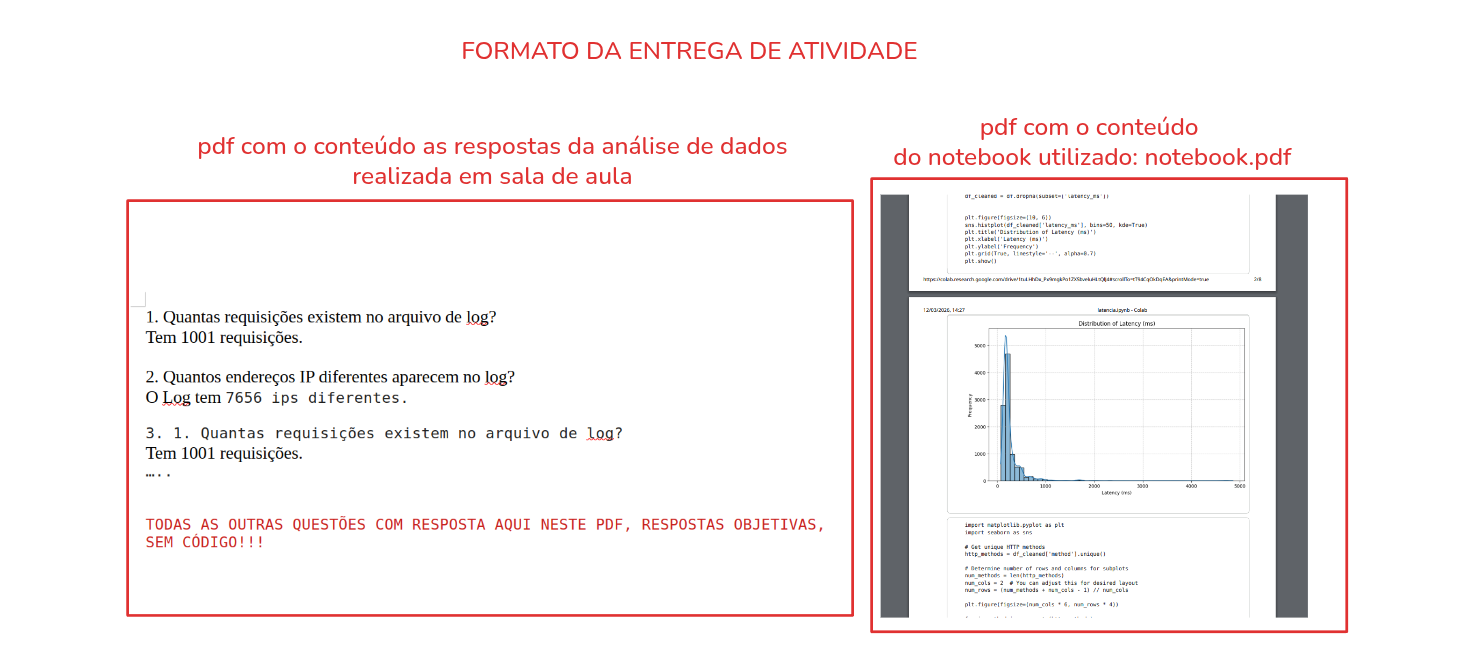
\includegraphics[width=\textwidth]{formato.png}
    \end{center}

\begin{block}{Parte 1 — Estrutura dos dados}

Responda:

\begin{enumerate}
\item Quantas requisições existem no arquivo de log?
\item Quantos endereços IP diferentes aparecem no log?
\item Quais métodos HTTP aparecem no conjunto de dados?
\item Qual o código de status mais frequente?
\end{enumerate}

\vspace{2cm}

\end{block}

\begin{block}{Parte 2 — Análise de latência}

Utilizando gráficos de distribuição:

\begin{enumerate}
\item Construa um histograma da latência das requisições.
\item Analise se a distribuição é simétrica ou assimétrica.
\item Existem requisições com latência muito elevada?
\item Qual é o percentil 90 da latência?
\end{enumerate}

\vspace{3cm}

\end{block}

\begin{block}{Parte 3 — Métodos HTTP}

\begin{enumerate}
\item Compare a distribuição de latência entre os métodos HTTP.
\item Algum método apresenta maior latência média?
\item Qual método apresenta maior variabilidade?
\end{enumerate}

\vspace{3cm}

\end{block}

\begin{block}{Parte 4 — Análise de erros e Confiabilidade}

Considere os códigos de status HTTP entre 400 e 599 como erros.

\begin{enumerate}
\item Quantas requisições resultaram em erro?
\item Calcule a \textbf{Taxa de Erro (Error Rate)} utilizando a fórmula:
\[ \text{Error Rate} = \frac{\text{Total de Erros}}{\text{Total de Requisições}} \times 100 \]
\item Calcule a \textbf{Disponibilidade (Availability)} do serviço:
\[ \text{Availability} = \frac{\text{Requisições com Sucesso}}{\text{Total de Requisições}} \times 100 \]
\item Compare a latência das requisições com erro e das requisições bem-sucedidas. O servidor demora mais para responder erros ou sucessos?
\end{enumerate}

\vspace{1cm}

\end{block}

\begin{block}{Parte 5 — SRE e SLAs (Service Level Agreements)}

A disponibilidade é frequentemente medida em "noves". Com base na tabela abaixo, em qual nível de disponibilidade o servidor se encontra?

\begin{center}
\begin{tabular}{|l|l|}
\hline
\textbf{Disponibilidade} & \textbf{Tempo fora do ar (por mês)} \\ \hline
99\% & $\sim$7h \\ \hline
99,9\% & $\sim$43 min \\ \hline
99,99\% & $\sim$4 min \\ \hline
99,999\% & $\sim$26 s \\ \hline
\end{tabular}
\end{center}

\begin{enumerate}
\item Se o acordo de nível de serviço (SLA) exigisse 99,9\% de disponibilidade, este servidor estaria cumprindo a meta?
\end{enumerate}

\end{block}

\begin{block}{Parte 6 — Requisições lentas}

Utilizando o percentil 90 de latência:

\begin{enumerate}
\item Identifique requisições com latência acima do percentil 90.
\item Quais URLs aparecem com maior frequência nessas requisições?
\item Existem IPs específicos associados a alta latência?
\end{enumerate}

\vspace{1cm}

\end{block}

\section*{Discussão}

Com base nas análises realizadas, responda:

\begin{itemize}
\item O servidor apresenta sinais de sobrecarga?
\item Existem indícios de acesso automatizado (bots)?
\item Quais possíveis melhorias poderiam ser aplicadas para reduzir a latência?
\end{itemize}

\vspace{4cm}

\chapter{Glossário de Termos Técnicos}

Este apêndice reúne as definições dos principais termos utilizados ao longo do livro, organizados em ordem alfabética para facilitar a consulta rápida.

\begin{description}[style=nextline, leftmargin=0pt]

    \item[ALARP (\textit{As Low As Reasonably Practicable})]
    Princípio de redução de riscos que estabelece que o risco deve ser reduzido ao mínimo razoavelmente praticável, considerando os custos e benefícios das medidas de mitigação.

    \item[Disponibilidade (\textit{Availability})]
    Propriedade de um sistema de estar operacional e acessível quando requerido. Geralmente expressa em porcentagem do tempo total (\emph{noves}: 99,9\%, 99,99\%, etc.).

    \item[Erro (\textit{Error})]
    Manifestação interna de uma falta no sistema. Um estado incorreto do sistema que pode ou não se propagar para uma falha observável externamente.

    \item[Engenharia de Confiabilidade de Sites — SRE (\textit{Site Reliability Engineering})]
    Conjunto de práticas de engenharia originadas no Google que aplicam princípios de software para problemas de infraestrutura e operações, visando sistemas escaláveis e altamente confiáveis.

    \item[Error Budget]
    Orçamento de erros definido como o complemento do SLO (ex: se o SLO é 99,9\%, o error budget é 0,1\%). Representa a quantidade de indisponibilidade tolerável em um dado período.

    \item[Falta (\textit{Fault})]
    Causa raiz de um erro. Pode ser um defeito no código, uma falha de hardware, um erro de configuração ou uma interferência ambiental. Também denominada \emph{defeito} ou \emph{bug}.

    \item[Falha (\textit{Failure})]
    Desvio do comportamento esperado externamente observável. Ocorre quando um erro se propaga até a saída do sistema, afetando o usuário ou sistema dependente.

    \item[FMEA (\textit{Failure Mode and Effects Analysis})]
    Análise de Modos de Falha e Efeitos. Técnica indutiva (\emph{bottom-up}) que examina cada componente do sistema individualmente para identificar seus modos de falha e os efeitos resultantes sobre o sistema.

    \item[FTA (\textit{Fault Tree Analysis})]
    Análise de Árvore de Falhas. Técnica dedutiva (\emph{top-down}) que parte de um evento indesejado (topo) e mapeia logicamente as combinações de falhas que podem causá-lo, usando portas AND/OR.

    \item[Perigo (\textit{Hazard})]
    Estado ou condição do sistema que possui potencial para causar um acidente. Difere do acidente em si, pois representa o risco latente antes que o dano ocorra.

    \item[Redundância]
    Estratégia de tolerância a falhas que consiste em replicar componentes críticos, de modo que a falha de um não comprometa o funcionamento do sistema.

    \item[Resiliência]
    Capacidade de um sistema de absorver perturbações, adaptar-se e continuar operando (ou recuperar-se rapidamente) após uma falha ou evento adverso.

    \item[Safety (Segurança Física)]
    Propriedade de um sistema de operar sem causar danos catastróficos a pessoas, ao meio ambiente ou ao patrimônio. Foca na proteção do mundo \emph{contra} o sistema.

    \item[Security (Segurança da Informação)]
    Propriedade de um sistema de resistir a acessos não autorizados, ataques deliberados e comprometimento da integridade dos dados. Foca na proteção do sistema \emph{contra} o mundo.

    \item[SLA (\textit{Service Level Agreement})]
    Acordo de Nível de Serviço. Contrato formal entre provedor e cliente que especifica os níveis mínimos de qualidade do serviço e as penalidades em caso de descumprimento.

    \item[SLI (\textit{Service Level Indicator})]
    Indicador de Nível de Serviço. Métrica quantitativa que mede um aspecto do serviço (ex: taxa de erros, latência, disponibilidade baseada em requisições).

    \item[SLO (\textit{Service Level Objective})]
    Objetivo de Nível de Serviço. A meta interna definida para um SLI (ex: latência P99 $\leq$ 300\,ms em 99,9\% do tempo).

    \item[TMR (\textit{Triple Modular Redundancy})]
    Redundância Modular Tripla. Arquitetura de tolerância a falhas onde três versões independentes de um componente executam em paralelo e um votador determina a saída correta por maioria.

    \item[Votador (\textit{Voter})]
    Componente de uma arquitetura redundante responsável por comparar as saídas dos canais redundantes e selecionar o resultado correto por votação majoritária.

\end{description}

%------------------------------------------------------------

\chapter{Tabela de Siglas e Acrônimos}

A tabela a seguir lista todas as siglas e acrônimos utilizados ao longo do livro, com suas formas expandidas em português e inglês onde aplicável.

\begin{table}[ht]
    \centering
    \renewcommand{\arraystretch}{1.4}
    \begin{tabular}{lp{5cm}p{6.5cm}}
        \toprule
        \textbf{Sigla} & \textbf{Forma Expandida (PT)} & \textbf{Forma Expandida (EN)} \\
        \midrule
        ALARP  & Tão Baixo Quanto Razoavelmente Praticável & As Low As Reasonably Practicable \\
        CAD    & Projeto Auxiliado por Computador          & Computer-Aided Design \\
        CI/CD  & Integração e Entrega Contínua             & Continuous Integration / Continuous Delivery \\
        FMEA   & Análise de Modos de Falha e Efeitos       & Failure Mode and Effects Analysis \\
        FTA    & Análise de Árvore de Falhas               & Fault Tree Analysis \\
        HTTP   & Protocolo de Transferência de Hipertexto  & Hypertext Transfer Protocol \\
        MTBF   & Tempo Médio Entre Falhas                  & Mean Time Between Failures \\
        MTTR   & Tempo Médio de Recuperação                & Mean Time to Repair / Recovery \\
        P99    & Percentil 99 de latência                  & 99th Percentile Latency \\
        RTOS   & Sistema Operacional de Tempo Real          & Real-Time Operating System \\
        SLA    & Acordo de Nível de Serviço                & Service Level Agreement \\
        SLI    & Indicador de Nível de Serviço             & Service Level Indicator \\
        SLO    & Objetivo de Nível de Serviço              & Service Level Objective \\
        SRE    & Engenharia de Confiabilidade de Sites      & Site Reliability Engineering \\
        TMR    & Redundância Modular Tripla                & Triple Modular Redundancy \\
        \bottomrule
    \end{tabular}
    \caption{Glossário de siglas e acrônimos utilizados no livro.}
\end{table}




\vspace{0.8cm}

\begin{center}
  \textit{``Boa atividade! Att. Me. Prof. Sergio Souza Novak.''}
\end{center}

%=============================================================
% REFERÊNCIAS BIBLIOGRÁFICAS
%=============================================================
\chapter*{Referências Bibliográficas}
\addcontentsline{toc}{chapter}{Referências Bibliográficas}
\printbibliography[heading=none]

\end{document}
